\documentclass[12pt, a4paper, ones, notitlepage, openany,titlepage]{article}
%Para el tamaño de las letras: 10pt, 11pt, 12pt
%Para el tamaño del papel: a4paper, letterpaper
%Forma de impresión: oneside or twoside
%Para el número de columnas: onecolumn, twocolumn
%Para que haya página de título o no: titlepage, notitlepage
%PAra la orientación de la página: portrait, landscape
%Para ecuaciones: leqno y fleqn

%Venian con el mathpix
\usepackage[utf8]{inputenc}
\usepackage[T1]{fontenc}
\usepackage{amsmath}
\usepackage{amsfonts}
\usepackage{amssymb}
\usepackage[version=4]{mhchem}
\usepackage{stmaryrd}
\usepackage{bbold}
\usepackage{graphicx}
\usepackage[export]{adjustbox}
\graphicspath{ {./images/} }

%Para enumerar con labels
\usepackage{enumitem}

\usepackage{mathtools}

\makeatletter
\renewcommand*\env@matrix[1][\arraystretch]{%
	\edef\arraystretch{#1}%
	\hskip -\arraycolsep
	\let\@ifnextchar\new@ifnextchar
	\array{*\c@MaxMatrixCols c}}
\makeatother

%Para cajas chulas
%\usepackage{tcolorbox}
\usepackage[utf8]{inputenc}

%Idioma
\usepackage[spanish]{babel}
%\usepackage[english]{babel}

%Salida
\usepackage[T1]{fontenc}

%Genera texto aleatorio
\usepackage{lipsum}
\usepackage{verbatim}

%Cambio de estilo y página
%\pagestyle{empty} %Sin nada
%\pagestyle{plain} %Número centrado en el pié
%\pagestyle{headings} %Con número y sección en la cabecera
%\pagestyle{myheadings} %personalizar

%Personalizar con myheadings
%\markright{Tema 0. Polinomios}{}
%\markboth{Álxebra Linear e Multilinear}{Francisco Estévez}

%Personalización con fancy
%\usepackage{fancyhdr}
%\pagestyle{fancy}
%%Cambios en las cabeceras
%\lhead[\leftmark]{{\footnotesize \leftmark}} %los corchetes son para la página izquierda y los brackets para la derecha
%%Cambios en los pies
%\chead[]{}
%\rhead[Xeometría Linear]{Xeometría Linear}
%\lfoot[Xeometría Linear]{Xeometría Linear} %los corchetes son para la página izquierda y los brackets para la derecha
%%Cambios en los pies
%\cfoot[\thepage]{\thepage}
%\rfoot[Francisco E. L.]{Francisco E. L.}

%Para personalizar cabeceras
\usepackage{fancyhdr}
%\rhead[]{}
%\lhead[\rightmark]{\rightmark}
%\lfoot[\thepage]{\thepage}
%\cfoot[]{}
%\rfoot[]{}
%\renewcommand{\headrulewidth}{0pt}
%\renewcommand{\footrulewidth}{0pt}
%\fancypagestyle{plain}{
	%	\fancyhf{}
	%	\fancyhead[L]{}
	%	\fancyfoot[L]{\thepage}
	%	\fancyhead[R]{Series Funcionais e Integración de Riemann en Varias Variables Reais}
	%	\renewcommand{\headrulewidth}{0pt}
	%	\renewcommand{\footrulewidth}{0pt}
	%}
%\pagestyle{fancy}

%Para sacar cabeceras en blanco


%Opciones predefinidas
%Número de página: \thepage
%Fecha del día: \today
%Palabra capítulo: \thechapter
%Título capítulo o seción (artículos): \leftmark 
%Para el título de la sección de libros o de la subseccións de artículos: \rightmark


%Numeración de páginas

\pagenumbering{arabic}
%Las opciones eran roman, Roman, arabic, alph, Alph


%Márgenes
%\topmargin 0.5 cm
%\headsep 0.5 cm
%\textheight 27cm
%\textwidth 18cm
\usepackage[left=0cm, right=0cm, top=1.00cm, bottom=1.00cm]{geometry}

\paperwidth=597.50787pt
\paperheight=845.04684pt
\textwidth=475pt
\textheight=650pt
\oddsidemargin=0pt
\evensidemargin=20pt
\topmargin=-14.31609pt
\headheight=15.0pt
\headsep=20pt
\headwidth=475pt
\topskip=12.0pt
\footskip=40.0pt
\marginparwidth=20.0pt
\marginparsep=7.0pt
\columnsep=10.0pt

%PAra que vayan bien las notas al margen
\usepackage{geometry}

%Para que las referencias sean linkeables
\usepackage[hidelinks]{hyperref} 
\hypersetup{
	colorlinks=true,
	linkcolor=black,
	%   filecolor=magenta,      
	urlcolor=blue,
	citecolor=black,
}


%Los principales paquetes matemáticos
\usepackage{amsmath}
\usepackage{amssymb}
\usepackage{amsthm}

%Para enumerar con letras
\usepackage{enumitem}

%Entornos tipo teorema
%\theoremstyle{plain}
%\newtheorem{teo}{Teorema}%También podría ser chapter
%\newtheorem{cor}{Corolario} %Enlazo Teoremas a corolarios
%\newtheorem{prop}{Proposición}
%\newtheorem{propi}{Propiedade}
%\newtheorem{lema}{Lema}
%\newtheorem{ax}{Axioma}
%
%\theoremstyle{definition}
%\newtheorem{defi}{Definición}
%
%\theoremstyle{remark}
%\newtheorem{exem}{Exemplo}
%\newtheorem{exer}{Exercicio}
%\newtheorem{obs}{Observación}
%\newtheorem{conc}{Conclusión}
%\newtheorem{nota}{Notación}

%No se lol
\usepackage{graphicx}
\usepackage{float}
\usepackage{subfigure}
\usepackage{wrapfig}

%Para colores
\usepackage[dvipsnames]{xcolor}

%\bibliographystyle{elsart-num}
%\bibliography{basededatosbiblio}
\usepackage[superscript, nomove]{cite}

%macros
\newcommand{\dobleimplicacion}[2]{
	\begin{enumerate}[label=$\Rightarrow/$]
		\item #1
	\end{enumerate}
	\begin{enumerate}[label=$\Leftarrow/$]
		\item #2
	\end{enumerate}
}
\newcommand{\doblecontenido}[2]{
	\begin{enumerate}[label=$\subset/$]
		\item #1
	\end{enumerate}
	\begin{enumerate}[label=$\supset/$]
		\item #2
	\end{enumerate}
}
\newcommand{\demostracion}{\noindent\underline{Demostración}}
\newcommand{\observacion}{\noindent\underline{\textbf{Observación}}}
\newcommand{\ejemplo}{\noindent\underline{\textbf{Ejemplo}}}
\newcommand{\ejemplos}{\noindent\underline{\textbf{Ejemplos}}}
\newcommand{\ejercicio}{\noindent\underline{\textbf{Ejercicio}}}

\newcommand{\distancia}[1]{\operatorname{d}(#1)}

\date{Curso 2022-2023}
\author{}
\makeglossary
\makeindex

\begin{document}
	
	\begin{titlepage}
		
		\centering
		{\scshape\LARGE Universidad de Santiago de Compostela \par}
		\vspace{1cm}
		{\scshape\Large Facultad de Matemáticas \par}
		\vspace{5cm}
		{\bfseries\scshape\Huge Geometría lineal\par}
		\vspace{12cm}
		
		{\Large Luis Barba Cepedello \par}
		\vfill
		{\Large Curso 2022-2023 \par}
	\end{titlepage}
	
	\setlength{\parskip}{0.30cm}
	
	\begin{center}
		\section{El Espacio Afín}
	\end{center}

En este tema introducimos el concepto de espacio afín como una generalización del plano y espacio ordinario. Cada espacio afín lleva asociado un espacio vectorial y en los espacios afines estudiamos únicamente las propiedades geométricas que se pueden deducir de las propiedades de sus vectores.

Un concepto fundamental en este tema es el paralelismo. La teoría de figuras homotéticas está dentro de la geometría afín. Los conceptos de traslación y homotecia y más en general el concepto de aplicación afín son conceptos afines. El estudio de longitudes, ángulos, perpendicularidad y distancias corresponde a la geometría euclídea.

Las figuras que utilizamos se refieren al plano o espacio ordinario y están aquí principalmente para apoyar nuestra intuición; las demostraciones deben hacerse de forma lógica y ser independientes de las figuras.

\subsection{Espacio afín sobre un espacio vectorial}
\noindent Sea $V$ un espacio vectorial sobre un cuerpo $K$.

\subsubsection{Definición - Espacio afín}
Un espacio afín sobre el espacio vectorial $V$ es una terna $(\mathbb{A}, V, \rightarrow)$ formada por un conjunto no vacío $\mathbb{A}$ cuyos elementos se llaman puntos, el espacio vectorial $V$ y una operación externa:
$$
\begin{aligned}
\rightarrow: \mathbb{A} \times \mathbb{A}: & \longrightarrow V \\
(P, Q) & \longmapsto \frac{V}{P Q}
\end{aligned}
$$
\begin{center}
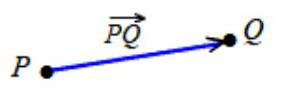
\includegraphics[max width=4cm]{2023_03_01_7659aec5e35f9a9b2d3cg-01(1)}
\end{center}

\noindent donde por $\overrightarrow{P Q}$ o también por $\overrightarrow{P, Q}$ denotamos la imagen por la aplicación $\rightarrow$ del par $(P, Q)$, verificándose los siguientes axiomas:

\begin{enumerate}
	\item Relación de Chasles: Para cualesquiera puntos $P, Q, R \in \mathbb{A}$, se verifica $\overrightarrow{P Q}+\overrightarrow{Q R}=\overrightarrow{P R}$.
	
	\begin{center}
	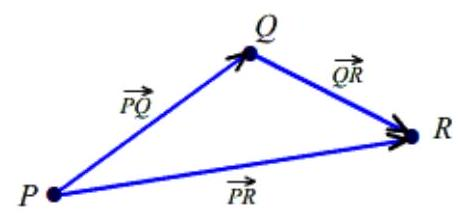
\includegraphics[max width=5cm]{2023_03_01_7659aec5e35f9a9b2d3cg-01}
	\end{center}
	
	\item Para cada punto $P \in \mathbb{A}$ y cada vector $v \in V$, existe un único punto $Q \in \mathbb{A}$ tal que $\overrightarrow{P Q}=v$; generalmente denotaremos $Q$ por $P+v$ y entonces se tiene que $\overrightarrow{P, P+v}=v$, para cada $P \in \mathbb{A}$ y cada $v \in V$.
	\begin{center}
		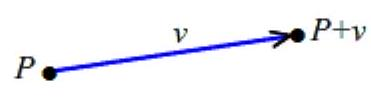
\includegraphics[max width=5cm]{2023_03_01_7659aec5e35f9a9b2d3cg-01(2)}
	\end{center}
\end{enumerate}

Con frecuencia denotaremos el espacio afín $(\mathbb{A}, V, \rightarrow)$ simplemente por $\mathbb{A}$. Si $K=\mathbb{R}$ diremos que $\mathbb{A}$ es un espacio afín real. Si $K=\mathbb{C}$ diremos que $\mathbb{A}$ es un espacio afín complejo.

\subsubsection{Proposición - Propiedades de un espacio afín}
\noindent Sea $\mathbb{A}$ un espacio afín sobre $V$. Se tiene:
\begin{enumerate}[label=(\arabic*)]
\item $P+\overrightarrow{P Q}=Q$, para todo $P, Q \in \mathbb{A}$

\item $\overrightarrow{P P}=0$, para todo $P \in \mathbb{A}$.

\item Si $\overrightarrow{P Q}=\overrightarrow{P Q^{\prime}} \Longrightarrow Q=Q^{\prime}$

\item $\overrightarrow{P Q}=0 \Longleftrightarrow Q=P$

\item $\overrightarrow{Q P}=-\overrightarrow{P Q}$, para todo $P, Q \in \mathbb{A}$.

\item Relación del paralelogramo: $\overrightarrow{P Q}=\overrightarrow{R T} \quad \Longrightarrow \quad \overrightarrow{P R}=\overrightarrow{Q T}$.

\begin{center}
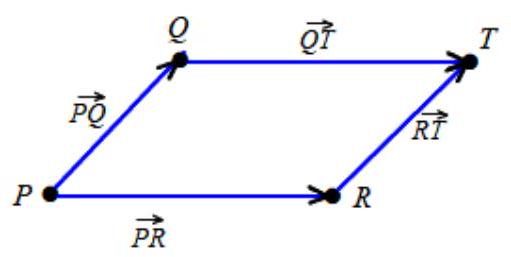
\includegraphics[max width=5cm]{2023_03_01_7659aec5e35f9a9b2d3cg-02}
\end{center}

\item Si $P+v=P+v^{\prime} \Rightarrow v=v^{\prime}$.

\item $P+(u+v)=(P+u)+v$, para todo $P \in \mathbb{A}$ y para cualesquiera $u, v \in V$.

\item $P+0=P$, para todo $P \in \mathbb{A}$.

\end{enumerate}

\noindent\underline{Demostración}
\begin{enumerate}[label=(\arabic*)]
\item $P + \overrightarrow{PQ}$ es, por el \textbf{\textit{Ax. 2}}, el único punto $R \in \mathbb{A} / \overrightarrow{PR} = \overrightarrow{PQ}$.

\item Dado que $\overrightarrow{P P}=\overrightarrow{P P}+\overrightarrow{P P}$, se tiene que $\overrightarrow{P P}=0$.

\item Pongamos $v=\overrightarrow{P Q}=\overrightarrow{P Q^{\prime}}$. Por la definición 1.1.1 (2), $Q=P+v=Q^{\prime}$.

\item Se sigue de (2) y (3).

\item Es consecuencia de que $\overrightarrow{P Q}+\overrightarrow{Q P}=\overrightarrow{P P}=0$.

\item Se tiene

$$
\overrightarrow{P R}=\overrightarrow{P Q}+\overrightarrow{Q R}=\overrightarrow{R T}+\overrightarrow{Q R}=\overrightarrow{Q R}+\overrightarrow{R T}=\overrightarrow{Q T}
$$

\item $v=\overrightarrow{P, P+v}=\overrightarrow{P, P+v^{\prime}}=v^{\prime}$.

\item Dado que

$$
\overrightarrow{P,(P+u)+v}=\overrightarrow{P, P+u}+\overrightarrow{P+u,(P+u)+v}=u+v=\overrightarrow{P, P+(u+v)}
$$

el resultado se sigue de (2).

\item Se sigue de (3), puesto que $\overrightarrow{P, P+0}=0=\overrightarrow{P P}$.
\end{enumerate}

\ejemplos
\begin{enumerate}
\item El conjunto de los puntos del plano (espacio) ordinario, junto con el espacio vectorial de los vectores libres del plano (espacio) y con la aplicación que lleva cada par de puntos $P, Q$ del plano (espacio) al vector libre $[\overrightarrow{P Q}]$, forman un espacio afín.

\item \textbf{Importante} Sea $V$ un espacio vectorial sobre $K$. La terna $(V, V, \rightarrow)$, donde para cualesquiera $P, Q \in V$, $\overrightarrow{P Q}=Q-P$, es un espacio afín. En efecto, la relación de Chasles se verifica puesto que

$$
\overrightarrow{P Q}+\overrightarrow{Q R}=(Q-P)+(R-Q)=R-P=\overrightarrow{P R}
$$

El axioma (2) se verifica, puesto que para cada punto $P \in V$ y cada vector $v \in V$ el punto $Q=P+v$ es el único punto que verifica la ecuación $Q-P=v$.

Así, todo espacio vectorial $V$ puede ser considerado como un espacio afín sobre $V$; este espacio afín se llama el espacio afín de $V$ y lo denotaremos por $V$.
\end{enumerate}

\subsection{Variedades lineales}

\subsubsection{Definición - Variedad lineal}
Sea $P$ un punto de $\mathbb{A}$ y sea $U$ un subespacio de $V$. Se llama variedad lineal o subespacio afín de $\mathbb{A}$ que pasa por $P$ y con dirección $U$ al conjunto
$$
P+U=\{P+u \mid u \in U\} \subset \mathbb{A}
$$
\begin{center}
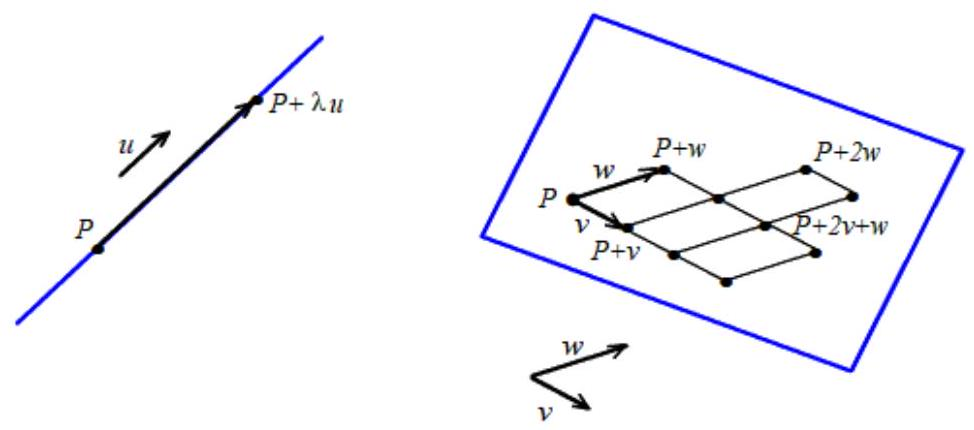
\includegraphics[max width=8cm]{2023_03_01_7659aec5e35f9a9b2d3cg-03}
\end{center}
\noindent A mayores, $\varnothing$ se considera variedad lineal.\\

\observacion

\noindent Las variedades lineales del espacio afín de $V$ son los subconjuntos de $V$ de la forma
$$
P+U=\{P+u \mid u \in U\}
$$
donde $P \in V$ y $U$ es un subespacio de $V$, es decir, son los elementos del espacio vectorial cociente $V / U$.

El espacio afín $\mathbb{A}$ sobre el espacio vectorial $V$ es una variedad lineal de $\mathbb{A}$. En efecto, $\mathbb{A}=P+V$, para todo $P \in \mathbb{A}$.

\subsubsection{Proposición - Propiedades de una variedad lineal}
\noindent Sea $\mathbb{A}$ un espacio afín sobre el espacio vectorial $V$.
\begin{enumerate}[label=(\arabic*)]
\item Sea $L=P+U$ una variedad lineal de $\mathbb{A}$ y $Q \in \mathbb{A}$. Son equivalentes:
\begin{enumerate}[label=(\alph*)]
\item $Q \in L$.
\item $\overrightarrow{P Q} \in U$.
\item $L=Q+U$.
\end{enumerate}
\item Sea $L=P+U$ una variedad lineal de $\mathbb{A}$. Si $R, S \in L$, entonces $\overrightarrow{R S} \in U$.
\item Sean $L_{1}=P_{1}+U_{1}$ y $L_{2}=P_{2}+U_{2}$ variedades lineales de $\mathbb{A}$. Se tiene
$$
L_{1} \subset L_{2} \quad \Longleftrightarrow \quad P_{1} \in L_{2}, \quad U_{1} \subset U_{2}
$$
\noindent y en particular,
$$
L_{1}=L_{2} \Rightarrow U_{1}=U_{2}
$$
\end{enumerate}

\demostracion
\begin{enumerate}[label=(\arabic*)]
\item 
\begin{enumerate}[label=(\alph*)]
	\item $\Rightarrow(b)$ Existe $u \in U$ tal que $Q=P+u$. Por tanto $\overrightarrow{P Q}=u \in U$.

	\item $ \Rightarrow(c)$ Para cada $u \in U$, se tiene
	$$
	P+u=Q+\overrightarrow{Q P}+u \in Q+U
	$$

	Así, $L \subset Q+U$. De forma similar se prueba que $Q+U \subset L$.

	\item $\Rightarrow(a)$ $Q=Q+0 \in Q+U=L$.
\end{enumerate}
\item Por (1) se tiene que $L=R+U$ y dado que $S \in R+U, \overrightarrow{R S} \in U$.

\item Si $L_{1} \subset L_{2}$, entonces $P_{1} \in L_{2}$ y por (1), $L_{2}=P_{1}+U_{2}$. Veamos que $U_{1} \subset U_{2}$. Si $u_{1} \in U_{1}$, $P_{1}+u_{1} \in L_{1} \subset L_{2}=P_{1}+U_{2}$, luego existe un vector $u_{2} \in U_{2}$ tal que $P_{1}+u_{1}=P_{1}+u_{2}$. De la proposición 1.1.2 (7), se sigue que $u_{1}=u_{2} \in U_{2}$. Recíprocamente, si $P_{1} \in L_{2}$, entonces $L_{2}=P_{1}+U_{2}$ y dado que $U_{1} \subset U_{2}$, se tiene $L_{1}=P_{1}+U_{1} \subset L_{2}$.
\end{enumerate}

\observacion

Como consecuencia de la proposición anterior, toda variedad lineal tiene un único subespacio dirección.

Veamos que toda variedad lineal es un espacio afín.

\subsubsection{Proposición - Relación entre variedad lineal y espacio afín}
Sea $L=P+U$ una variedad lineal de $\mathbb{A}$. La terna $(L, U, \rightarrow)$, siendo $\rightarrow: L \times L \longrightarrow U$ la aplicación que lleva cada par $(Q, R) \in L \times L$ al vector $\overrightarrow{Q R}$ de $V$, es un espacio afín sobre $U$.

\demostracion

Dado que $Q, R \in L$, el vector $\overrightarrow{Q R} \in U$, por lo que la aplicación está bien definida. La relación de Chasles se verifica para los puntos de $L$, puesto que se verifica para los puntos de $\mathbb{A}$. También se verifica el axioma (2), puesto que para cada punto $Q \in L$ y cada vector $u \in U$ el punto $R=Q+u \in L=Q+U$ es el único punto que verifica la ecuación $\overrightarrow{Q R}=u$.

\subsubsection{Definición - Combinación lineal}
Sea $V$ un espacio vectorial sobre $K$. Una combinación lineal de los elementos $v_{1}, \ldots, v_{r} \in V$ es una suma
$$
\sum_{i=1}^{r} \lambda_{i} v_{i}, \quad \lambda_{i} \in K, \quad i=1, \ldots, r .
$$

Si $S$ es un subconjunto de $V$, se llama subespacio generado por $S$, y se denota por $\langle S\rangle$, al conjunto de todas las combinaciones lineales de los elementos de todos los subconjuntos finitos de $S$. Si $S$ es un subconjunto de $V$, entonces $\langle S\rangle$ es el menor subespacio de $V$ que contiene a $S$.

\observacion

Una base de un espacio vectorial $V$ de dimensión $n$ es una $n$-pla $\left(v_{1}, \ldots, v_{n}\right) \in V^{n}$ tal que el conjunto $\left\{v_{1}, \ldots, v_{n}\right\}$ genera $V$; en particular, los vectores $v_{1}, \ldots, v_{n}$ son linealmente independientes.

\subsubsection{Definición - Dimensión de un espacio afín}
Se llama dimensión del espacio afín $(\mathbb{A}, V, \rightarrow)$ a la dimensión de $V$ como espacio vectorial sobre $K$. Si $\mathbb{A}$ es un espacio afín y $L=P+U$ es una variedad lineal de $\mathbb{A}$, entonces $\dim  L=\dim _{K} U$.

\subsubsection{Definición - Rectas, planos e hiperplanos}
Se llaman rectas y planos a los espacios afines de dimensiones 1 y 2, respectivamente. Si la dimensión de $\mathbb{A}$ es $n$, se llaman hiperplanos de $\mathbb{A}$ a las variedades lineales de dimensión $n-1$. El espacio afín $\mathbb{A}$ tiene dimensión 0 si, y solo si, $\mathbb{A}=\{P\}$, para algún $P \in \mathbb{A}$. El conjunto vacío se considera una variedad lineal de dimensión $-1$.

\subsubsection{Proposición - Relación entre variedades lineales con su dimensión}
Si $L_{1}=P_{1}+U_{1}$ y $L_{2}=P_{2}+U_{2}$ son variedades lineales de igual dimensión de un espacio afín $\mathbb{A}$ y $L_{1} \subset L_{2}$, entonces $L_{1}=L_{2}$.

\demostracion

Como $L_1 \subset L_2$, $U_{1} \subset U_{2}$ y $P_{1} \in L_{2}$. Dado que $\dim _{K} U_{1}=\dim _{K} U_{2}$, se tiene que $U_{1}=U_{2}$ y entonces, $L_{2}=P_{1}+U_{2}=P_{1}+U_{1}=L_{1}$.

\subsection{Unión e intersección de variedades lineales}

\subsubsection{Proposición - Intersección de variedades lineales}
Sea $\mathbb{A}$ un espacio afín sobre $V$. Si $\left\{L_{i}\right\}_{i \in I}$ es un conjunto de variedades lineales de $\mathbb{A}$, entonces $\displaystyle\bigcap_{i \in I} L_{i}$ es una variedad lineal de $\mathbb{A}$. Es más, si $L_{i}=P_{i}+U_{i}$ y $Q \in \displaystyle \bigcap_{i \in I} L_{i}$,
$$
\bigcap_{i \in I} L_{i}=Q+\bigcap_{i \in I} U_{i}
$$

\demostracion
\begin{itemize}
	\item Si $\displaystyle\bigcap_{i \in I} L_i = \varnothing$, es una variedad lineal por definición.
	\item Si $\displaystyle\bigcap_{i \in I}L_i \neq \varnothing \Longrightarrow \exists Q \in \bigcap_{i \in I}L_i$. Llega con probar que $\displaystyle \bigcap_{i \in I}L_i = Q + \bigcap_{i \in I}U_i$. Notar que $\displaystyle Q \in \bigcap_{i \in I}L_i \Longrightarrow Q \in L_i, \forall i \in I \Longrightarrow L_i = Q + U_i$. Así:
	\begin{gather*}
		P \in \bigcap_{i \in I} L_{i} \Longleftrightarrow P \in L_{i} = Q + U_i, \; \forall i \in I \Longleftrightarrow \overrightarrow{Q P} \in U_{i}, \; \forall i \in I \Longleftrightarrow \\
		\Longleftrightarrow \overrightarrow{Q P} \in \bigcap_{i \in I} U_{i} \Longleftrightarrow P \in Q+\bigcap_{i \in I} U_{i} .
	\end{gather*}
	
\end{itemize}
Como consecuencia, si $\displaystyle \bigcap_{i \in I} L_{i} \neq \varnothing$, entonces $\displaystyle 
\dim \left(\bigcap_{i \in I} L_{i}\right)=\dim _{K}\left(\bigcap_{i \in I} U_{i}\right)$.

\subsubsection{Definición - Variedad lineal generada}
Si $S \subset \mathbb{A}$ es un subconjunto de puntos, se llama variedad lineal generada por $S$ y la denotaremos por $\langle\langle S\rangle\rangle$ a la variedad lineal
$$
\langle\langle S\rangle\rangle=\bigcap_{i \in I} L_{i}
$$
\noindent Donde $\left\{L_{i}\right\}_{i \in I}$ es el conjunto de variedades lineales de $\mathbb{A}$ que contienen a $S$.

\noindent\underline{Observaciones}
\begin{itemize}
\item La variedad lineal generada por $S$ es la menor variedad lineal de $\mathbb{A}$ que contiene a $S$.
\item $\langle\langle \varnothing \rangle\rangle = \varnothing$.
\item $\langle\langle P \rangle\rangle = \{P\} = P + \{0\}$.
\end{itemize}
La siguiente proposición da una descripción de los elementos de $\langle\langle S\rangle\rangle$.

\subsubsection{Proposición - Caracterización de los elementos de $\langle\langle S\rangle\rangle$}
\noindent Si $S \neq \varnothing$ un subconjunto de $\mathbb{A}$, entonces
$$
\langle\langle S\rangle\rangle=Q+\langle\overrightarrow{Q R} \mid R \in S\rangle
$$
\noindent para cualquier $Q \in S$.

\demostracion

\noindent La inclusión $S \subset Q+\langle\overrightarrow{Q R} \mid R \in S\rangle$ se sigue de las igualdades
$$
Q=Q+0, \quad R=Q+\overrightarrow{Q R}, \quad \forall R \in S
$$
Pues si $P \in S \Longrightarrow P = Q + \overrightarrow{QP} \in Q + \langle \{\overrightarrow{QR} \mid R \in S\} \rangle$.

Veamos que es el menor. Sea $L_1$ una variedad lineal de $\mathbb{A}$ tal que $S \subset L_1$. Denotemos $L = Q + \langle\{\overrightarrow{QR} \mid R \in S\}\rangle$. Tenemos que ver que $L \subset L_1$.
$$
Q \in S \subset L_1 \Longrightarrow L_1 = Q + U.
$$
Si $P \in S \subset L_1 \Longrightarrow \overrightarrow{QP} \in U$. Por tanto,
$$
\{\overrightarrow{QR} \mid R \in S\} \subset U \Longrightarrow \langle \{\overrightarrow{QR} \mid R \in S\} \rangle \subset U \Longrightarrow Q + \langle\{\overrightarrow{QR} \mid R \in S\}\rangle \subset Q + U = L_1
$$

\ejercicio
	
\noindent Sean $S$ y $S^{\prime}$ subconjuntos no vacíos de $\mathbb{A}$. Prueba que:
\begin{enumerate}[label=(\arabic*)]
\item $S \subset\langle\langle S\rangle\rangle$.

\item Si $S \subset S^{\prime}$, entonces $\langle\langle S\rangle\rangle \subset\left\langle\left\langle S^{\prime}\right\rangle\right\rangle$.

\item $S$ es una variedad lineal de $\mathbb{A}$ si, y solo si, $\langle\langle S\rangle\rangle=S$.

\item Si $\mathbb{A}$ tiene dimensión finita, existe un subconjunto finito $S_{0}$ de $S$ tal que $\langle\langle S\rangle\rangle=\left\langle\left\langle S_{0}\right\rangle\right\rangle$.

\item Dados $P, Q \in \mathbb{A}$, si $Q \in\langle\langle S \cup\{P\}\rangle\rangle$ y $Q \notin\langle\langle S\rangle\rangle$, entonces $P \in\langle\langle S \cup\{Q\}\rangle\rangle$.
\end{enumerate}

\subsubsection{Proposición - Propiedades de $\langle\langle S\rangle\rangle$}
\noindent Sea $\mathbb{A}$ un espacio afín sobre $V$ y sean $S, S' \subset \mathbb{A} \mid S \neq \varnothing \neq S'$. Se verifican:
\begin{enumerate}[label=(\alph*)]
	\item Si $S \subset S' \Longrightarrow \langle\langle S \rangle\rangle \subset \langle\langle S' \rangle\rangle$.
	\item $S$ es una variedad lineal $\Longleftrightarrow S = \langle\langle S \rangle\rangle$.
	\item Si $\mathbb{A}$ tiene dimensión finita, entonces existe un subconjunto finito $S_0$ de $S \mid \langle\langle S_0 \rangle\rangle = \langle\langle S \rangle\rangle$.
	\item Dados $P, Q \in \mathbb{A}$, entonces si $Q \in \langle\langle S \cup \{P\} \rangle\rangle$ y $Q \notin \langle\langle S \rangle\rangle$ entonces $P \in \langle\langle S \cup \{Q\}\rangle\rangle$.
\end{enumerate}
\demostracion
\begin{enumerate}[label=(\alph*)]
	\item Como $S' \subset \langle\langle S' \rangle\rangle$ y $S \subset S'$, entonces $S \subset \langle\langle S' \rangle\rangle$. Puesto que $\langle\langle S \rangle\rangle$ es la menor variedad lineal que contiene a $S$, se tiene que $\langle\langle S \rangle\rangle \subset \langle\langle S' \rangle\rangle$.
	\item ''$\Longrightarrow$''. Veamos el doble contenido. $S \subset \langle\langle S \rangle\rangle$ se cumple siempre, queda ver ''$\supset$''. Puesto que $S \subset S$ y $S$ es variedad lineal, entonces $\langle\langle S \rangle\rangle \subset S$ por ser $\langle\langle S \rangle\rangle$ la menor variedad lineal que contiene a $S$.
	
	''$\Longleftarrow$''. $\langle\langle S \rangle\rangle$ es variedad lineal $\Longrightarrow S = \langle\langle S \rangle\rangle$ es variedad lineal.
	\item Por ser $S \neq \varnothing, \; \exists Q \in S \subset \langle\langle S \rangle\rangle$. Por tanto, $\langle\langle S \rangle\rangle = Q + U$. Como $U \subset V$ y $V$ tiene dimensión finita, entonces $U$ tiene dimensión finita. Tomemos entonces $\{u_1,\ldots,u_r\}$ una base de $U$. Sean $P_i = Q + u_i, \; i = 1,\ldots,r \Longleftrightarrow \overrightarrow{QP_i} = u_i$. Tomemos ahora $S_0 = \{Q, P_1, \ldots, P_r\}$.
	$$
	\begin{aligned}
		\langle\langle S_0 \rangle\rangle & = Q + \langle\langle \{\overrightarrow{QP_i} \mid P_i \in S_0\} \rangle\rangle = \\ & = Q + \langle\langle \{\overrightarrow{QP_1},\ldots,\overrightarrow{QP_r}\} \rangle\rangle = \\ & = Q + \langle\langle \{u_1,\ldots,u_r\} \rangle\rangle = \\ & = Q + U = \langle\langle S \rangle\rangle
	\end{aligned}
	$$
	\item Como $Q \in \langle\langle S \cup \{P\} \rangle\rangle$ y $Q \notin \langle\langle S \rangle\rangle$, se tiene que $P \in \langle\langle S \rangle\rangle$. Puesto que $S \neq \varnothing \Longrightarrow \exists T \in S \Longrightarrow \langle\langle S \rangle\rangle = T + \langle \{\overrightarrow{TR} \mid R \in S\} \rangle$. Ahora bien, $S \subset S \cup \{P\} \Longrightarrow T \in S \cup \{P\}$. Así, $\langle\langle S \cup \{P\} \rangle\rangle = T + \langle \{\overrightarrow{TR} \mid R \in S \cup \{P\}\} \rangle = T + \langle \{\overrightarrow{TR} \mid R \in S\} \rangle + \langle \{\overrightarrow{TP}\} \rangle$.
	
	Por hipótesis, $\displaystyle Q \in \langle\langle S \cup \{P\}\rangle\rangle \Longleftrightarrow \overrightarrow{TQ} \in \langle \{\overrightarrow{TR} \mid R \in S\} \rangle + \langle \overrightarrow{TP} \rangle \Longrightarrow \exists \{R_1,\ldots,R_r\} \subset S \text{ finito } \mid \overrightarrow{TQ} = \sum_{i = 1}^{r} \lambda_i \overrightarrow{TR_i} + \mu \overrightarrow{TP} \text{ con } \lambda_i, \mu \in \mathbb{R}$. Veamos que $\displaystyle \mu \neq 0$. Si $\displaystyle \mu = 0 \Longrightarrow \overrightarrow{TQ} = \sum_{i = 1}^{r} \lambda_i \overrightarrow{TR} \Longrightarrow Q \in \langle\langle S \rangle\rangle$, lo cual es una contradicción.
	
	Podemos dividir por $\mu$. $\displaystyle \overrightarrow{TP} = \frac{1}{\mu} \overrightarrow{TQ} + \sum_{i = 1}^{r} \frac{-\lambda_i}{\mu} \overrightarrow{TR} \in \langle \{\overrightarrow{TR}\} \rangle + \langle \{\overrightarrow{TR} | R \in S\} \rangle \Longrightarrow \\ P \in T + \langle \{\overrightarrow{TR} \mid R \in S \cup \{Q\}\} \rangle = \langle\langle S \cup \{Q\} \rangle\rangle$.
\end{enumerate}

\subsubsection{Proposición - $\varnothing$ como intersección de variedades lineales}
\noindent Sean $L_{1}=P_{1}+U_{1}$ y $L_{2}=P_{2}+U_{2}$ variedades lineales de $\mathbb{A}$. Se tiene
$$
L_{1} \cap L_{2} \neq \varnothing \quad \Longleftrightarrow \quad \overrightarrow{P_{1} P_{2}} \in U_{1}+U_{2}
$$

\demostracion

Si $L_{1} \cap L_{2} \neq \varnothing$, existen $u_{1} \in U_{1}$ y $u_{2} \in U_{2}$ tales que $P_{1}+u_{1}=P_{2}+u_{2}$. Entonces $P_{1}=P_{2}+u_{2}-u_{1}$, de donde se sigue que $\overrightarrow{P_{1} P_{2}}=u_{1}-u_{2} \in U_{1}+U_{2}$.

Recíprocamente, si $\overrightarrow{P_{1} P_{2}} \in U_{1}+U_{2}$, existen vectores $u_{1} \in U_{1}$ y $u_{2} \in U_{2}$ tales que $\overrightarrow{P_{1} P_{2}}=u_{1}+u_{2}$, luego $P_{2}=P_{1}+\overrightarrow{P_{1} P_{2}}=P_{1}+u_{1}+u_{2}$. Por tanto $P_{2}-u_{2}=P_{1}+u_{1} \in L_{1} \cap L_{2}$.

\observacion

Si $L_{1}$ y $L_{2}$ son variedades lineales de $\mathbb{A}$ su unión conjuntista $L_{1} \cup L_{2}$ no es, en general, una variedad lineal de $\mathbb{A}$.

\subsubsection{Proposición - Unión de variedades lineales como variedad lineal}
Sea $\mathbb{A}$ un espacio afín sobre un $K$ espacio vectorial, donde el cuerpo $K$ tiene característica distinta de 2 y sean $L_{1}$ y $L_{2}$ variedades lineales. Entonces, si $L_1 \cup L_2$ es una variedad lineal, se tiene que o bien $L_{1} \subset L_{2}$ o bien $L_{2} \subset L_{1}$.

\demostracion

En efecto, sean $L_{1}=P_{1}+U_{1}$ y $L_{2}=P_{2}+U_{2}$ y supongamos que $U$ es el subespacio dirección de $L_{1} \cup L_{2}$. Dado que $P_{1}, P_{2} \in L_{1} \cup L_{2}$, se tiene que $\overrightarrow{P_{1} P_{2}} \in U$, luego
$$
P_{1}+2 \overrightarrow{P_{1} P_{2}} \in L_{1} \cup L_{2}
$$
\noindent Si $P_{1}+2 \overrightarrow{P_{1} P_{2}} \in L_{1}$, entonces $2 \overrightarrow{P_{1} P_{2}} \in U_{1} \xRightarrow{\operatorname{car}(K) \neq 2} \overrightarrow{P_1 P_2} \in U_1$. Por otro lado, si $P_{1}+2 \overrightarrow{P_{1} P_{2}} \in L_{2} \Longrightarrow \overrightarrow{P_{1} P_{2}}=\overrightarrow{P_{2} P_{1}}+2 \overrightarrow{P_{1} P_{2}}=\overrightarrow{P_{2}, P_{1}+2 \overrightarrow{P_{1} P_{2}}} \in L_2$.

En todo caso, $\overrightarrow{P_{1} P_{2}} \in L_{1} \cup L_{2}$, de donde se sigue que $\overrightarrow{P_1 P_2} \in U_1 \cup U_2 \subset \langle U_1 \cup U_2 \rangle = U_1 + U_2 \Longrightarrow L_1 \cup L_2 \neq \varnothing$. Sea $P \in L_1 \cup L_2 \Longrightarrow \begin{cases}
	L_1 \cup L_2 = P + U \\
	L_1 = P + U_1 \\
	L_2 = P + U_2
\end{cases}$ \\
Veamos que $U = U_1 + U_2$
\begin{enumerate}[label=$\subset/$]
	\item Sea $u \in U \Longrightarrow P + u \in L_1 \cup L_2$. Casos:
	\begin{itemize}
		\item Si $P + u \in L_1 \Longleftrightarrow u = \overrightarrow{P,P+u} \in U_1$
		\item Si $P + u \in L_2 \Longleftrightarrow u = \overrightarrow{P,P+u} \in U_2$
	\end{itemize}
	En virtud de lo anterior, $u \in U_1 \cup U_2$.
\end{enumerate}
\begin{enumerate}[label=$\supset/$]
	\item \begin{itemize}
	\item Sea $u_1 \in U_1 \Longrightarrow P + u_1 \in L_1 \subset L_1 \cup L_2 \Longrightarrow \overrightarrow{P,P+u} = \overrightarrow{P,u_1} \in U$
	\item Sea $u_2 \in U_2 \Longrightarrow P + u_2 \in L_2 \subset L_1 \cup L_2 \Longrightarrow \overrightarrow{P,P+u} = \overrightarrow{P,u_2} \in U$
	\end{itemize}
\end{enumerate}
Luego $U = U_1 \cup U_2$. Por ser $U$ un subespacio vectorial se tiene que $\begin{cases}
	U_1 \subset U_2 \\
	o \\
	U_2 \subset U_1
\end{cases}$ \\
Por tanto, $P \in L_1 \cap L_2 \Longrightarrow \begin{cases}
	L_1 \subset L_2 \\
	o \\
	L_2 \subset L_1
\end{cases}$

\subsubsection{Definición - Variedad unión o suma}
Sea $\left\{L_{i}\right\}_{i \in I}$ un conjunto de variedades lineales de $\mathbb{A}$. Se llama variedad lineal unión o suma de las variedades $\left\{L_{i}\right\}_{i \in I}$ de $\mathbb{A}$ a la menor variedad lineal de $\mathbb{A}$ que contiene a $\displaystyle \bigcup_{i \in I} L_{i}$; la denotaremos por $\circ_{i \in I} L_{i}$. Se tiene
$$
\circ_{i \in I} L_{i}=\left\langle\left\langle\bigcup_{i \in I} L_{i}\right\rangle\right\rangle
$$
Si la familia es finita $\{L_1,\ldots,L_r\}$, escribiremos $L_1 \circ \ldots \circ L_r$. En particular, si $L_i=P_i \in \mathbb{A}$, escribiremos $P_{1} \circ \ldots \circ P_{r}=\langle\langle S\rangle\rangle$ en vez de $\{P_1\} \circ \ldots \circ \{P_r\} = \langle\langle S\rangle\rangle$.

\noindent La siguiente proposición da una expresión sencilla de los elementos de $L_{1} \circ L_{2}$.

\subsubsection{Proposición - Caracterización de los elementos de la variedad suma}
Si $L_{1}=P_{1}+U_{1}$ y $L_{2}=P_{2}+U_{2}$ son variedades lineales de $\mathbb{A}$, entonces
$$
L_{1} \circ L_{2}=P_{1}+\left\langle\overrightarrow{P_{1} P_{2}}\right\rangle+U_{1}+U_{2}
$$

\demostracion

\begin{enumerate}[label=$\subset/$]
	\item Sea $u_1 \in U_1 \Longrightarrow P_1 + u_1 \in P_1 + \langle \overrightarrow{P_1 P_2} \rangle + U_1 + U_2$. Sea $u_2 \in U_2 \Longrightarrow P_2 + u_2 = P_1 + \overrightarrow{P_1 P_2} + u_2 \in P_1 + \langle \overrightarrow{P_1 P_2} \rangle + U_1 + U_2$. Se tiene que $L_1 \cup L_2 \subset P_1 + \langle \{P_1 P_2\} \rangle + U_1 + U_2$. Así, $L_1 \circ L_2 = \langle\langle L_1 \cup L_2 \rangle\rangle \subset P_1 + \langle \{P_1 P_2\} \rangle + U_1 + U_2$ es la menor variedad lineal que contiene a $L_1$ y $L_2$.
\end{enumerate}
\begin{enumerate}[label=$\supset/$]
	\item Sea $L = Q + U$ una variedad lineal cumpliendo $L_1 \cup L_2 \subset L$.
	$$
	\left. \begin{array}{r}
		L_1 \subset L \Longrightarrow U_1 \subset U \\
		L_2 \subset L \Longrightarrow U_2 \subset U
	\end{array} \right\} \Longrightarrow U_1 \cup U_2 \subset U \Longrightarrow U_1 + U_2 \subset U
	$$
\end{enumerate}

\subsubsection{Corolario - Propiedades de la dimensión de espacios intersección y suma}
Sea $\mathbb{A}$ un espacio vectorial de dimensión finita y sean $L_{1}=P_{1}+U_{1}$ y $L_{2}=P_{2}+U_{2}$ variedades lineales de $\mathbb{A}$. Se tiene:
\begin{enumerate}[label=(\arabic*)]
\item Identidad de Grassman para variedades lineales afines: Si $L_{1} \cap L_{2} \neq \varnothing$, entonces
$$
\dim \left(L_{1} \circ L_{2}\right)+\dim \left(L_{1} \cap L_{2}\right)=\dim  L_{1}+\dim  L_{2} .
$$

\item Si $L_{1} \cap L_{2}=\varnothing$, entonces
$$
\dim \left(L_{1} \circ L_{2}\right)=1+\dim _{K}\left(U_{1}+U_{2}\right) .
$$
\end{enumerate}
\demostracion
\begin{enumerate}[label=(\arabic*)]
\item Si $L_{1} \cap L_{2} \neq \varnothing \Longrightarrow \exists Q \in L_{1} \cap L_{2}$, entonces $L_{1} \cap L_{2} = Q + \langle \{\overrightarrow{QQ}\} \rangle + U_1 + U_2 = Q+\left(U_{1} \cap U_{2}\right)$. Por otro lado, $L_{1} \circ L_{2}=$ $P_{1}+U_{1}+U_{2}$. El resultado se sigue de la identidad de Grassman para subespacios:
\begin{gather*}
\dim  (L_1 \circ L_2) + \dim  (L_1 \cap L_2) \overset{def}{=} \dim _K (U_1 + U_2) + \dim _K (U_1 \cap U_2) \\ \overset{Grassman}{=} \dim _K (U_1) + \dim _K (U_2) = \dim  (L_1) + \dim  (L_2)
\end{gather*}

\item Si $L_{1} \cap L_{2}=\varnothing$, entonces $\overrightarrow{P_{1} P_{2}} \notin U_{1}+U_{2}$ y por tanto $\left\langle\overrightarrow{P_{1} P_{2}}\right\rangle \cap\left(U_{1}+U_{2}\right)=\{0\}$. Así, $\dim \left(L_{1} \circ L_{2}\right) = \dim _K \left(\langle\{\overrightarrow{P_1 P_2}\} \rangle \oplus (U_1 + U_2)\right) =1+\dim _{K}\left(U_{1}+U_{2}\right)$.
\end{enumerate}

\subsection{Posiciones relativas de variedades lineales}

\subsubsection{Definición - Relación de paralelismo}
Se dice que las variedades lineales $L_{1}=P_{1}+U_{1}$ y $L_{2}=P_{2}+U_{2}$ son paralelas, si $U_{1} \subset U_{2}$ o $U_{2} \subset U_{1}$. Se escribe $L_{1} \| L_{2}$.

\subsubsection{Proposición - Propiedades del paralelismo}
\noindent Sean $L=Q+U, L_{1}=P_{1}+U_{1}$ y $L_{2}=P_{2}+U_{2}$ variedades lineales de $\mathbb{A}$. Se tiene:
\begin{enumerate}[label=(\arabic*)]
\item Si $L_{1} \| L_{2}$ y $\dim  L_{1}=\dim  L_{2}$, entonces $U_{1}=U_{2}$.

\item Si $L_{1} \| L_{2}$ y $L_{1} \cap L_{2} \neq \varnothing$, entonces $L_{1} \subset L_{2}$ o $L_{2} \subset L_{1}$; además, si $\dim  L_{1}=\dim  L_{2}$, entonces $L_{1}=L_{2}$

\item La ''relación de paralelismo'' es una relación de equivalencia en el conjunto de las variedades lineales de la misma dimensión de un espacio afín.

\item Axioma del paralelismo. Si $P$ es un punto de $\mathbb{A}$ tal que $P \notin L$, entonces existe una única variedad lineal $L^{\prime}$ de la misma dimensión que $L$ que pasa por $P$ y es paralela a $L$.

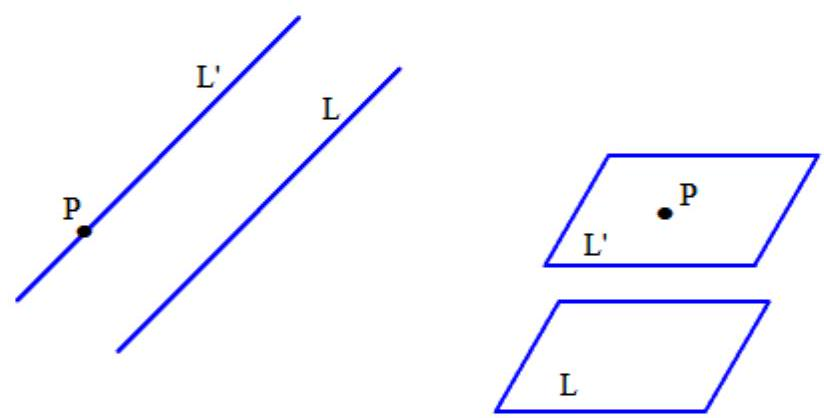
\includegraphics[max width=7cm, center]{2023_03_01_7659aec5e35f9a9b2d3cg-08}

\item Si $L_{1} \| L_{2}$ y $\dim  L_{1} \leq \dim  L_{2}$, entonces existe una única variedad lineal $L^{\prime \prime}$ tal que $\dim  L^{\prime \prime}=$ $\dim  L_{2}, L_{1} \subset L^{\prime \prime}$ y $L^{\prime \prime} \| L_{2}$.
\end{enumerate}

\demostracion
\begin{enumerate}[label=(\arabic*)]
\item Dado que $U_{1} \subset U_{2}$ y $\dim _{K} U_{1}=\dim _{K} U_{2}$, se tiene que $U_{1}=U_{2}$.

\item Si $Q \in L_{1} \cap L_{2}$, entonces $L_{1}=Q+U_{1}$ y $L_{2}=Q+U_{2}$. Dado que $L_{1} \| L_{2}$, se tiene $U_{1} \subset U_{2}$ o $U_{2} \subset U_{1}$. Así, $L_{1} \subset L_{2}$ o $L_{2} \subset L_{1}$.

\item \begin{itemize}
	\item Reflexiva
	$$
	L \| L \text{ ya que } U \subset U
	$$
	\item Simétrica
	$$
	L_1 \| L_2 \Longleftrightarrow \left\{\begin{array}{r}
		U_1 \subset U_2 \\
		U_2 \subset U_1
	\end{array}\right\} \Longleftrightarrow L_2 \| L_1
	$$
	\item Transitiva
	$$
	\left.\begin{array}{r}
		L_1 \| L_2 \xRightarrow{\dim L_1 = \dim L_2} U_1 = U_2 \\
		L_2 \| L_3 \xRightarrow{\dim L_2 = \dim L_3} U_2 = U_3
	\end{array}\right\} \Longrightarrow U_1 = U_3 \Longrightarrow L_1 \| L_3
	$$
\end{itemize}

\item Sean $L = Q + U, \; P \notin L$
\begin{itemize}
	\item Existencia
	$$
	L' = P + U \Longrightarrow P \in L' \text{ y } \dim L = \dim L' = \operatorname{U}
	$$
	\item Unicidad. Sea $L'$ variedad lineal con $\dim L' = \dim L$ y $P \in L'$.
	$$
	\left.\begin{array}{r}
		P \in L' \Longrightarrow L' = P + U' \\
		L \| L' \xRightarrow{\dim L = \dim L'} U = U'
	\end{array}\right\} \Longrightarrow L' = P + U
	$$
\end{itemize}

\item Sean $L_1 \| L_2, \mid \dim L_1 \le \dim  L_2, \; L_1 = P_1 + U_1, \; L_2 = P_2 + U_2$
\begin{itemize}
	\item Existencia y unicidad. Tomemos $L'' = P_1 + U_2$. $L''$ es único, ya que contiene $P_1$ y es paralela a $L_2$, por \textbf{(4)}. Tenemos que probar que $L_1 \subset L''$. Como $L_1 \| L_2$,
	$$
	\left.\begin{array}{r}
		U_1 \subset U_2  \\
		\text{o} \\
		U_2 \subset U_1
	\end{array}\right\} \Longrightarrow U_1 \subset U_2 \Longrightarrow L_1 = P_1 + U_1 \subset P_1 + U_2 = L''
	$$
\end{itemize}
\end{enumerate}

\subsubsection{Definición - Cortarse, cruzarse y pasar por}
\noindent Sean $L_{1}$ y $L_{2}$ variedades lineales del espacio afín $\mathbb{A}$ sobre $V$.
\begin{enumerate}[label=(\arabic*)]
\item Se dice que $L_{1}$ y $L_{2}$ se cortan si $L_{1} \cap L_{2} \neq \varnothing$.
\item Se dice que $L_{1}$ y $L_{2}$ se cruzan si no son paralelas y no se cortan.
\item Si $P$ es un punto de $\mathbb{A}$, diremos que la variedad lineal $L$ pasa por $P$ si $P \in L$.
\end{enumerate}
\observacion

El apartado \textbf{(2)} prueba que dos variedades lineales de la misma dimensión paralelas y distintas no se cortan:
$$
L \| L' \text{ y } L \neq L' \Longrightarrow L \cap L' = \varnothing
$$
\noindent Es más, sean $L_1$ y $L_1$ variedades lineales, entonces
$$
\text{Como } L_1 \| L_2 \text{ y } \begin{array}{r}
	L_1 \not\subset L_2 \\
	L_2 \not\subset L_1
\end{array} \Longrightarrow L_1 \cap L_2 = \varnothing
$$

\ejemplo

Sea el espacio afín $\mathbb{R^3}$ Consideramos las rectas $r_{a}=(0,1,1)+\langle(-1,2, a)\rangle$ y $s_{a}=(1,0,1)+\langle(a-1,4,-2)\rangle$, y vamos a estudiar la posición relativa de $r_{a}$ y $s_{a}$ según los valores de $a \in \mathbb{R}$.
Paralelismo. Las rectas $r_{a}$ y $s_{a}$ son paralelas si, y solo si, $\langle(-1,2, a)\rangle=\langle(a-1,4,-2)\rangle$. Por tanto,
$$
r_{a} \| s_{a} \Longleftrightarrow \lambda(-1,2, a)=(a-1,4,-2) \text { para algún } \lambda \in \mathbb{R} \Longleftrightarrow a=-1 .
$$
De esta forma,
$$
r_{a} \cap s_{a} \neq \varnothing \Longleftrightarrow(1,-1,0) \in\langle(-1,2, a),(a-1,4,-2)\rangle
$$
y si $a \neq-1$,
$$
r_{a} \cap s_{a} \neq \varnothing \Longleftrightarrow\left|\begin{array}{rrr}
1 & -1 & a-1 \\
-1 & 2 & 4 \\
0 & a & -2
\end{array}\right|=0 \Longleftrightarrow a=-2 .
$$
Así, $r_{-1} \| s_{-1}, r_{-2} \cap s_{-2} \neq \varnothing, r_{-2} \neq s_{-2}$ y $r_{a}$ y $s_{a}$ se cruzan para todo $a \in \mathbb{R}-\{-1,-2\}$. Además, $r_{-2} \cap s_{-2}=\{(-1 / 2,2,0)\}$

\subsubsection{Proposición - Axioma de la recta}
\noindent Sea $\mathbb{A}$ un espacio afín sobre el espacio vectorial $V$. Se tiene:
\begin{center}
	''Por dos puntos distintos pasa una única recta''
\end{center}

\demostracion

\noindent Sean $P, Q \in \mathbb{A} \mid P \neq Q$.
\begin{itemize}
	\item Existencia: $P, Q \in P \circ Q = \langle\langle \{P,Q\} \rangle\rangle$. Veamos que $P \circ Q$ es una recta.
	$$
	P \circ Q = P + \langle\{\overrightarrow{PQ}\}\rangle \text{. Como } P \neq Q \Longrightarrow \overrightarrow{PQ} \neq 0 \Longrightarrow \dim P \circ Q = 1
	$$
	\item Unicidad: Sea $L \subset \mathbb{A} \text{ recta } \,/\, P,Q \in L$.
	$$
	P,Q \in L \Longrightarrow \{P,Q\} \subset L \Longrightarrow P \circ Q \subset L \xRightarrow{\dim P \circ Q = 1 = \dim L} L = P \circ Q
	$$
\end{itemize}
\observacion

\noindent Que existan dos puntos distintos implica que $\dim \mathbb{A} > 1$.

\subsubsection{Proposición - Axioma de incidencia entre recta y plano}
\noindent Sea $\mathbb{A}$ un espacio afín sobre $V$. Se tiene:
\begin{center}
	''Si dos puntos distintos de una recta están en un plano, entonces la recta está en el plano''
\end{center}
\demostracion

Sean $L \subset \mathbb{A}$ una recta y $\pi \subset \mathbb{A}$ un plano $/\, \{P,Q\} \subset L \cap \pi, \; P \neq Q$. Como $P \neq Q \Longrightarrow L = P \circ Q$, por la proposición anterior. Así, $\{P,Q\} \subset \pi \Longrightarrow L = P \circ Q \subset \pi$.

\observacion

\noindent Notar que la existencia de un plano en $\mathbb{A}$ implica que $\dim \mathbb{A} \ge 2$.

\subsubsection{Lema - Tres puntos no alineados son distintos}
Sea $A$ un espacio afín sobre $V$. Si $\dim \mathbb{A} \ge 1$, se tiene que si $P,Q,R \in \mathbb{A}$ son no alineados, entonces $P \neq Q \neq R \neq P$.

\demostracion

Lo probaremos por reducción al absurdo. Supongamos que al menos dos de los puntos son iguales ($P = Q$).
\begin{itemize}
	\item $P \neq R \Longrightarrow P = Q, \; R \in P \circ R \text{ recta } \Longrightarrow \text{ son alineados }$. Contradicción.
	\item $P = Q = R$, como $\dim_K V \ge 1 \Longrightarrow \exists v \in V \,/\, v \neq 0$. Tomemos entonces $L = P + \langle\{v\}\rangle, \; \dim L = 1$ y $P = Q = R \in L \Longrightarrow \text{ son alineados }$. Contradicción.
\end{itemize}

\observacion

El Lema anterior no es cierto para $\dim \mathbb{A} = 0$. Tomemos $\mathbb{A} = \{P\}$. Al no existir rectas, $P,P,P$ son no alineados pero iguales.

\subsubsection{Proposición - Axioma del plano}
\noindent Sea $\mathbb{A}$ un espacio afín sobre $V$. Entonces si $\dim \mathbb{A} \ge 1$, se tiene:
\begin{center}
	''Por tres puntos no alineados pasa un único plano''
\end{center}
\demostracion

\noindent Sean $P,Q,R \in \mathbb{A}$ no alineados.
\begin{itemize}
	\item Existencia: Tomemos $P = Q = R$ y veamos que es un plano. $P \circ Q \circ R = P + \langle\{\overrightarrow{PQ},\overrightarrow{PR}\}\rangle$ es un plano $\Longrightarrow \overrightarrow{PQ}$ y $\overrightarrow{PR}$ son linealmente independientes. Supongamos lo contrario: $\exists \lambda \in K \,/\, \overrightarrow{PQ} = \lambda \overrightarrow{PR} \Longrightarrow P \circ Q \circ R = P + \langle\{\overrightarrow{PQ}\}\rangle$ es una recta. Entonces, $P, Q, R \in P + \langle\{\overrightarrow{PQ}\}\rangle \Longrightarrow P,Q,R$ están alineados. Contradicción.
	
	\item Unicidad. Sea $\pi \text{ plano } /\, P,Q,R \in \pi \Longrightarrow P \circ Q \circ R \subset \pi \xRightarrow{ \dim P \circ Q \circ R = \dim \pi = 2 } P \circ Q \circ R = \pi$.
\end{itemize}
\observacion

\noindent Que existan 3 puntos no alineados distintos implica que $\dim \mathbb{A} \ge 2$.

\subsubsection{Teorema - Incidencia de variedades lineales en el plano}
Sea $\mathbb{A}$ un plano afín ($\dim \mathbb{A} = 2$) sobre $V$. Entonces, dos rectas son paralelas si, y solo si, no se cortan.

\demostracion
\begin{enumerate}[label=$\Longrightarrow/$]
	\item $$
	\left. \begin{array}{r}
		L \| L' \\
		L \neq L' \\
		\dim L = \dim L'
	\end{array} \right\} \Longrightarrow L \cap L' = \varnothing
	$$
\end{enumerate}
\begin{enumerate}[label=$\Longleftarrow/$]
	\item $L \cap L' = \varnothing \Longleftrightarrow \overrightarrow{PP'} \notin \langle\{u\}\rangle + \langle\{v\}\rangle = \langle\{u,v\}\rangle$. Ahora bien, $L = P + \langle\{u\}\rangle$ y $L' = P' + \langle\{v\}\rangle$. Como $\dim_K V = 2 \Longrightarrow \dim_K \langle\{u,v\}\rangle = 1 \Longrightarrow \langle\{u\}\rangle = \langle\{v\}\rangle \Longleftrightarrow L = L'$.
\end{enumerate}
\observacion
\noindent Si $\dim \mathbb{A} = 2$, entonces no existen rectas que se crucen.

\subsubsection{Teorema - Incidencia de variedades lineales en el e.a. tridimensional}
\noindent Sea $\mathbb{A}$ un espacio afín de $\dim = 3$.
\begin{enumerate}[label=(\alph*)]
	\item Axioma de incidencia plano-plano en dimensión $3$. Se tiene:
	\begin{center}
		''Si dos planos se cortan, su intersección es una recta''
	\end{center}
	\item Dos planos distintos son paralelos si, y solo si, no se cortan.
	\item Un plano y una recta no contenida en el plano son paralelos si, y solo si, no se cortan.
	\item Dos rectas distintas son paralelas si, y solo si, son coplanarias y no se cortan.
\end{enumerate}
\demostracion
\begin{enumerate}[label=(\alph*)]
	\item Sean $\pi$ y $\pi'$ planos, $\pi \neq \pi'$ y $\pi \cap \pi' \neq \varnothing$. Dado que $\pi \neq \pi'$, se tiene que $\pi \subset \pi \circ \pi'$ y si $\pi = \pi \circ \pi' \Longrightarrow \pi' \subset \pi \Longrightarrow \pi' = \pi$. Ahora, como $\pi \not\subseteq \pi \circ \pi' \Longrightarrow \dim \pi < \dim(\pi \circ \pi')$
	$$
	\left. \begin{array}{r}
		\Longrightarrow \dim \pi \circ \pi' > 2 \\
		\pi \circ \pi' \subset \mathbb{A} \Longrightarrow \dim(\pi \circ \pi') \le 3
	\end{array} \right\} \Longrightarrow \dim(\pi \circ \pi') = 3
	$$
	Como $\pi \cap \pi' \neq \varnothing$, usando Grassmann:
	$$
	\dim(\pi \cap \pi') = \dim(\pi) + \dim(\pi') - \dim(\pi - \pi') = 2 + 2 - 3 = 1
	$$
	
	\item Sean $\pi = P + U$ y $\pi' = P' + U'$ planos distintos.
	\dobleimplicacion{Ya visto}{
	$\pi \cap \pi' = \varnothing \Longrightarrow \dim(\pi \circ \pi') = 1 + \dim_K (U + U')$. Por otro lado, $\pi \circ \pi' \subset \mathbb{A} \Longrightarrow \dim(\pi \circ \pi') \le 3$. Así,
	$$
	\left. \begin{array}{r}
		\Longrightarrow \dim_K (U + U') \le 2 \\
		\dim_K (U) = \dim_K (U') \\
		U \subset U + u'
	\end{array} \right\} \Longrightarrow U = U + u' = u' \Longrightarrow \pi \| \pi'
	$$}
	
	\item Sean $L = P + \langle\{v\}$ y $\pi = Q + U$ un plano tal que $L \not\subset \pi$
	\dobleimplicacion{Ya probada}{
	$L \cap \pi' = \varnothing$. Por Grassmann, $\dim (L \circ \pi) = 1 + \dim_K (\langle\{v\} + U \rangle)$. Como $L \circ \pi \subset A$, entonces $\dim (L \circ \pi) \le 3$. Así, $\dim_K (\langle\{v\} + U \rangle) \le 2 \Longrightarrow v \in U$.
	}
	
	\item
	\dobleimplicacion
	{Sean $L = P + \langle\{u\}\rangle$ y $L' = Q + \langle\{u\}\rangle$ paralelas, $L \neq L'$. Ya sabemos que $L \cap L' = \varnothing$, queda ver que son coplanarias. Como $L \cap L' = \varnothing$, $\dim (L \circ L') = 1 + \dim_K (\langle \{u\} \rangle) \Longrightarrow \dim (L \circ L') = 2$. Por tanto, $L, L' \subset L \circ L'$ es un plano.}
	{Si $L = P + \langle\{u\}\rangle$ y $L' = Q + \langle\{v\}$ son distintas y coplanarias. Tomamos el plano $\pi$ como el plano afín en el que trabajan. Tenemos dos rectas que no se cortan en el plano afín, por tanto son paralelas ($L\|L'$).}
\end{enumerate}
\observacion

En el apartado (d) hemos probado que si $L$ y $L'$ son rectas paralelas distintas, entonces $L \circ L'$ es un plano. Además, si $L \circ L' \subset \pi$ es un plano, entonces $L \circ L' \subset \pi \Longrightarrow \pi = L \circ L'$, es decir, por dos rectas pasa un único plano.

\subsection{Referencias afines y coordenadas}
Sea $V$ un espacio vectorial sobre un cuerpo $K$ y $\mathbb{A}$ un espacio afín sobre el espacio vectorial $V$. En esta sección se introducen coordenadas en el espacio afín $\mathbb{A}$ y se estudian las ecuaciones lineales de las variedades lineales de $\mathbb{A}$.

\subsubsection{Definición - Puntos afinmente independientes}
Se dice que $P_{1}, \ldots, P_{r} \in \mathbb{A}$ son afinmente independientes si los vectores $\overrightarrow{P_{1} P_{2}}, \ldots, \overrightarrow{P_{1} P_{r}}$ son linealmente independientes.

\subsubsection{Proposición - Propiedades de los puntos afinmente independientes}
\noindent Sea $\mathbb{A}$ un espacio afín sobre $V$.
\begin{enumerate}[label=(\arabic*)]
\item Sean $P_{1}, \ldots, P_{r} \in \mathbb{A}$. Son equivalentes:
\begin{enumerate}[label=(\alph*)]
	\item $P_{1}, \ldots, P_{r}$ son afínmente independientes.

	\item $\dim  P_{1} \circ \ldots \circ P_{r}=r-1$.

	\item $P_{i} \notin P_{1} \circ \ldots \circ \widehat{P}_{i} \circ \ldots \circ P_{r}, i=1, \ldots, r$, donde con $\widehat{P}_{i}$ indicamos que se elimina el punto $P_{i}$.
\end{enumerate}

\item Los puntos $P_{1}, \ldots, P_{r}$ son afínmente independientes si, y solo si, los puntos $P_{\sigma(1)}, \ldots, P_{\sigma(r)}$ son afínmente independientes para toda permutación $\sigma \in S_{r}$.

\item Si $P_1,\ldots,P_r$ son afínmente independientes y $P \notin P_1 \circ \ldots \circ P_r$, entonces los puntos $P_1, \ldots P_r, P$ son afínmente independientes.

\item Si $P_1, \ldots, P_r$ son afínmente independientes, entonces $P_1, \ldots, \widehat{P_i}, \ldots, P_r$ son afínmente independientes.
\end{enumerate}
\demostracion
\begin{enumerate}[label=(\arabic*)]
	\item \begin{enumerate}[label=(\alph*)]
		\item $\Longleftrightarrow$ (b). Se tiene que
		\begin{gather*}
			P_1 \circ \ldots \circ P_r = P_1 + \langle \{\overrightarrow{P_1 P_2}\}, \ldots, \{\overrightarrow{P_1 P_r}\} \rangle
		\end{gather*}
		Por tanto,
		\begin{gather*}
			P_1 \circ \ldots \circ P_r \text{ son a.i. } \xLeftrightarrow{\text{definición}} \overrightarrow{P_1 P_2}, \ldots, \overrightarrow{P_1 P_r} \text{ son l.i. } \Longleftrightarrow \\ \Longleftrightarrow \dim_K (\langle \{\overrightarrow{P_1 P_2}\}, \ldots \{\overrightarrow{P_1 P_r}\}\rangle) = r - 1 \Longleftrightarrow \dim(P_1 \circ \ldots \circ P_r) = r - 1
		\end{gather*}
		\item $\Longleftrightarrow$ (c). Sea $i \in \{2, \ldots r\}$.
		$$
		\begin{aligned}
			& P_1, \ldots P_2 \text{ son a.i. } \Longleftrightarrow \overrightarrow{P_1 P_2}, \ldots, \overrightarrow{P_1 P_r} \text{ son l.i. } \Longleftrightarrow \\
			& \Longleftrightarrow \overrightarrow{P_1 P_i} \notin \langle \{\overrightarrow{P_1 P_2}, \ldots, \overrightarrow{P_1 P_i}, \ldots, \overrightarrow{P_1 P_r}\} \Longleftrightarrow \\
			& \Longleftrightarrow P_i \notin P_1 + \langle \{\overrightarrow{P_1 P_2}, \ldots, \overrightarrow{P_1 P_i}, \ldots, \overrightarrow{P_1 P_r}\} \Longleftrightarrow \\
			& \Longleftrightarrow P_i \notin P_1 \circ \ldots \widehat{P_i} \circ \ldots \circ P_r
		\end{aligned}
		$$
		En caso de que $i = 1$, reordenamos usando (2).
	\end{enumerate}

	\item $P_1 \circ \ldots \circ P_r = \langle\langle \{P_1, \ldots, P_r\} \rangle\rangle = P_{\sigma(1)}, \ldots, P_{\sigma(r)}$, de donde
	$$
	r - 1 = \dim(P_1 \circ \ldots \circ P_r) = \dim(P_{\sigma(1)}, \ldots, P_{\sigma(r)})
	$$
	
	\item Se tiene:
	$$
	\begin{aligned}
	& P \notin P_1 \circ \ldots \circ P_r \Longrightarrow \notin P_1 + \langle \{\overrightarrow{P_1 P_2}, \ldots, \overrightarrow{P_1 P_r}\} \rangle \Longleftrightarrow \\
	& \Longleftrightarrow \overrightarrow{P_1 P} \notin \langle \{\overrightarrow{P_1 P_2}, \ldots, \overrightarrow{P_1 P_r}\} \rangle \Longleftrightarrow \\
	& \Longleftrightarrow \overrightarrow{P_1 P_2}, \ldots \overrightarrow{P_1 P_r}, \overrightarrow{P_1 P} \text{ son l.i. } \Longleftrightarrow \\
	& \Longleftrightarrow P_1, \ldots, P_2, P \text{ son a.i. }
	\end{aligned}
	$$

	\item Supongamos que $i \neq 1$. Si $i = 1$, reordenamos usando (2).
	$$
	\begin{aligned}
		& P_1, \ldots, P_r \text{ son a.i. } \xLeftrightarrow{\text{definición}} \overrightarrow{P_1 P_2}, \ldots \overrightarrow{P_1 P_r} \text{ son l.i. } \Longrightarrow \\
		& \Longrightarrow P_1, \ldots, \widehat{\overrightarrow{P_1 P_i}}, \ldots, \overrightarrow{P_1 P_r} \text{ son l.i. } \Longleftrightarrow \\
		& \Longleftrightarrow P_1, \ldots, \widehat{P_i}, \ldots, P_r \text{ son a.i. }
	\end{aligned}
	$$
\end{enumerate}

\subsubsection{Proposición - Relación entre ser afines y ser no alineados}
\noindent Sea $\mathbb{A}$ un espacio afín sobre $V$. Entonces,
\begin{enumerate}[label=(\arabic*)]
	\item Dos puntos $P_1, P_2 \in \mathbb{A}$ son afínmente independientes si, y solo si, $P_1 \neq P_2$.
	\item Si $\dim(\mathbb{A}) \ge 1$, tres puntos $P_1, P_2, P_3 \in \mathbb{A}$ son afínmente independientes si, y solo si, son no alineados.
	\item Si $\dim(\mathbb{A}) \ge 2$, cuatro puntos $P_1, P_2, P_3, P_4 \in \mathbb{A}$ son afínmente independientes si, y solo si, son no alineados.
\end{enumerate}
\demostracion
\begin{enumerate}[label=(\arabic*)]
	\item Como $P_1 \neq P_2$, entonces $\overrightarrow{P_1 P_2} \neq 0 \Longleftrightarrow P_1 + \langle\{\overrightarrow{P_1 P_2}\}\rangle \dim(P_1 \circ P_2) = 1 \Longleftrightarrow P_1, P_2$ son afínmente independientes.
	\item \dobleimplicacion{Por contrarrecíproco.
	Si $P_1, P_2, P_3$ son alineados $\Longrightarrow \exists L \subset \mathbb{A}$ recta $/\, P_1, P_2, P_3 \in L \Longrightarrow P_1 \circ P_2 \circ P_3 \subset L \Longrightarrow \dim P_1 \circ P_2 \circ P_3 \le 1 \Longrightarrow P_1, P_2, P_3$ son afínmente independientes.
	}{Reducción al absurdo.
	Supongamos que $P_1, P_2, P_3$ no son afínmente independientes. Entonces, $\dim (P_1 \circ P_2 \circ P_3) = 1$. Ahora,
	\begin{itemize}
		\item Si $\dim(P_1 \circ P_2 \circ P_3) = 1 \Longrightarrow P_1, P_2, P_3 \in P_1 \circ P_2 \circ P_3$ recta. Contradicción.
		\item Si $\dim (P_1 \circ P_2 \circ P_3) = 0 \Longrightarrow P_1 = P_2 = P_3$. Como $\dim_K V \ge 1 \Longrightarrow \exists v \in V \,/\, v \neq 0$. Tomemos $P_1 + \langle\{v\}\rangle = L$ recta. $P_1 = P_2 = P_3 \in L$. Contradicción.
	\end{itemize}
	}
	\item \dobleimplicacion{Por contrarrecíproco.
	Si $P_1, P_2, P_3, P_4$ son alineados $\Longrightarrow \exists \pi \subset \mathbb{A}$ plano $/\, P_1, P_2, P_3, P_4 \in \pi \Longrightarrow P_1 \circ P_2 \circ P_3 \circ P_4 \subset \pi \Longrightarrow \dim P_1 \circ P_2 \circ P_3 \circ P_4 \le 2 \Longrightarrow P_1, P_2, P_3, P_4$ son afínmente independientes.
	}{Reducción al absurdo.
	Supongamos que $P_1, P_2, P_3, P_4$ no son afínmente independientes. Entonces, $\dim (P_1 \circ P_2 \circ P_3 \circ P_4) \le 2$. Ahora,
	\begin{itemize}
		\item Si $\dim(P_1 \circ P_2 \circ P_3 \circ P_4) = 2 \Longrightarrow P_1, P_2, P_3, P_4 \in P_1 \circ P_2 \circ P_3 \circ P_4$ plano. Contradicción.
		\item Si $\dim (P_1 \circ P_2 \circ P_3 \circ P_4) = 1 \Longrightarrow P_1 \circ P_2 \circ P_3 \circ P_4$ recta, luego $P_1 \circ P_2 \circ P_3 \circ P_4 = P_1 + \langle\{u\}\rangle, \; u \in V-\{0\}$. Como $\dim_K V \ge 2, \; \exists v \in V \,/\, u, v$ son linealmente independientes. Tomamos $\pi = P_1 + \langle\{u,v\}\rangle$ plano. Es claro que $P_1, P_2, P_3, P_4 \in P_1 \circ P_2 \circ P_3 \circ P_4 \subset \pi$. Contradicción.
		\item Si $\dim (P_1 \circ P_2 \circ P_3 \circ P_4) = 0 \Longrightarrow P_1 = P_2 = P_3 = P_4$. Como $\dim_K V \ge 2 \Longrightarrow \exists u,v \in V \,/\, u,v$ son linealmente independientes. Tomemos $\pi = P_1 + \langle\{u,v\}\rangle = L$ plano. $P_1 = P_2 = P_3 = P_4 \in \pi$. Contradicción.
	\end{itemize}
	}
\end{enumerate}
\observacion
\begin{itemize}
	\item Si $\dim \mathbb{A} \ge 1 \Longrightarrow$ dado $P \in \mathbb{A}, \; \exists L \subset \mathbb{A}$ recta $/\, P \in L$.
	\item Si $\dim \mathbb{A} \ge 2 \Longrightarrow$ dado $P \in \mathbb{A}, \; \exists \pi \subset \mathbb{A}$ recta $/\, P \in \pi$.
	\item Si $\dim \mathbb{A} \ge 2 \Longrightarrow$ dada $L \subset \mathbb{A}$ recta, $\exists \pi \subset \mathbb{A}$ plano $/\, P \in L$.
\end{itemize}
\observacion
\begin{itemize}
	\item Si $\dim \mathbb{A} = 0$, entonces $P, P, P$ son no alineados y no coplanarios. Sin embargo, $\dim(P) = 0 \neq 2 \Longleftrightarrow P,P,P$ son no afínmente independientes. También, $\dim(P) = 0 \neq 3 \Longleftrightarrow P,P,P,P$ son no afínmente independientes.
	\item Si $\dim \mathbb{A} = 1$, entonces $P,P,P,P$ son no coplanarios pero no son afínmente independientes. Es más, si $P \neq Q, \; \{P_1,P_2,P_3,P_4\}$ con $P_1 \in \{P,Q\}$ son no coplanarios y no son afínmente independientes.
\end{itemize}

\subsubsection{Proposición - Relación entre número de puntos a.i. y la dimensión de $\mathbb{A}$}
\noindent Sea $\mathbb{A}$ un espacio afín sobre $V$.
\begin{enumerate}[label=(\arabic*)]
\item Si la dimensión de $\mathbb{A}$ es $n$, entonces $\mathbb{A}$ tiene $n+1$ puntos afínmente independientes. Es más, el mayor número de puntos afínmente independientes es $n+1$.

\item Si $P_{1}, \ldots, P_{n+1}$ son puntos de $\mathbb{A}$ afínmente independientes y $\dim  \mathbb{A}=n$, entonces $\mathbb{A}=P_{1} \circ \ldots \circ P_{n+1}$.

\item Si la dimensión de $\mathbb{A}$ es $n$ y $P_{1}, \ldots P_{r}, \; r \leq n+1$, son puntos afínmente independientes, entonces existen puntos $P_{r+1}, \ldots, P_{n+1}$ tales que $P_{1}, \ldots, P_r, P_{r+1}, \ldots, P_{n+1}$ son afínmente independientes.
\end{enumerate}
\demostracion
\begin{enumerate}[label=(\arabic*)]
\item Veamos que existen $n+1$ puntos afínmente independientes. Si $P$ es un punto de $\mathbb{A}$ y $\left(v_{1}, \ldots, v_{n}\right)$ es una base de $V$, entonces los puntos $P, P+v_{1}, \ldots, P+v_{n}$ son $n+1$ puntos afínmente independientes. Así
$$
\left\{\overrightarrow{P, P + v_1}, \ldots, \overrightarrow{P, P + v_n}\right\} = \{v_1, \ldots, v_n\} \text{ son l.i.} \Longrightarrow P, P + v_1, \ldots, P + v_n \text{ son a.i.}
$$
Por otro lado, sean $P_1, \ldots P_r$ afínmente independientes. Entonces,
$$
\dim(P_1 \circ P_r) = r - 1 \le n \Longrightarrow r \le n + 1
$$

\item Dado que $\dim \left(P_{1} \circ \ldots \circ P_{n+1}\right)=n = \dim \mathbb{A}$ y que $P_1 \circ \ldots \circ P_{n + 1} \subset A$, entonces $\mathbb{A}=P_{1} \circ \ldots \circ P_{n+1}$.

\item Sean $P_1, \ldots, P_r$ afínmente independientes. Por definición, $\overrightarrow{P_1,P_2}, \ldots, \overrightarrow{P_1,P_r}$ son $r - 1$ vectores linealmente independientes. Como $\dim_K V = r, \; \exists v_r, \ldots, v_n \in V \,/\, \overrightarrow{P_1, P_2}, \ldots, \overrightarrow{P_1 P_r}, \\ v_r, \ldots, v_n$ forman una base de $V \Longrightarrow P_1, \ldots, P_r, P_1 + v_r, \ldots, P_1 + v_n$ son $n + 1$ puntos afínmente independientes.
\end{enumerate}

\observacion \; - Axioma de dimensión
\begin{itemize}
	\item ''Toda recta tiene dos puntos distintos''
	\item ''Todo plano tiene tres puntos distintos no alineados''
\end{itemize}
\demostracion
\begin{enumerate}
	\item $\mathbb{A}$ recta $\Longrightarrow \exists P,Q \in \mathbb{A}$ afínmente independientes $\Longrightarrow P \neq Q$.
	\item $\mathbb{A}$ plano $\Longrightarrow \exists P_1, P_2, P_3$ afínmente independientes tales que son no alineados. Como $P_i, P_j$ con $i \neq j$ son afínmente independientes, $P_i \neq P_j, \; i \neq j$.
\end{enumerate}
Queda probado que todo espacio afín de dimensión $3$ tiene $4$ puntos distintos no coplanarios, cada $3$ no alineados.

\observacion \; - Axioma de intersección plano-plano

Si dos planos se cortan en al menos un punto en $\dim \mathbb{A} = 3$, entonces hemos visto que se cortan en una recta. Como toda recta tiene $2$ puntos distintos, entonces se cortan en al menos otro punto distinto del anterior.

\noindent Con esto, \underline{ya se han probado todos los axiomas del espacio afín.}

\subsubsection{Definición - Referencia o referencia afín}
Sea $\mathbb{A}$ un espacio afín de dimensión $n$. Una referencia o referencia afín $\mathcal{R}$ de $\mathbb{A}$ es una $(n+1)$-pla $\left(P_{1}, \ldots, P_{n}, Q\right)$ de $\mathbb{A}^{n+1}$ tal que los puntos $P_{1}, \ldots, P_{n}, Q$ son afínmente independientes. Escribiremos $\mathcal{R}=\left\{P_{1}, \ldots, P_{n} ; Q\right\}$ y diremos que $Q$ es el origen y $B_{\mathcal{R}}=\left(\overrightarrow{Q P_{1}}, \ldots, \overrightarrow{Q P_{n}}\right)$ es la base asociada a $\mathcal{R}$.

Los siguientes dibujos muestran una referencia en el plano y una referencia en el espacio afín tridimensional, respectivamente.

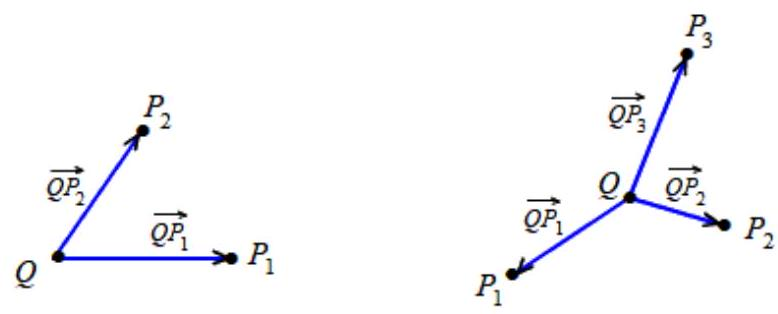
\includegraphics[max width=8cm, center]{2023_03_01_7659aec5e35f9a9b2d3cg-11}
\observacion

\noindent Todo espacio afín tiene, al menos, una referencia.

\ejemplos
\begin{enumerate}[label=(\arabic*)]
\item La referencia canónica $\mathcal{C}=\left\{E_{1}, E_{2} ; O\right\}$ del plano ordinario es una terna $\left(E_{1}, E_{2}, O\right)$ de puntos no alineados tal que las rectas $O \circ E_{1}$ y $O \circ E_{2}$ son perpendiculares, los vectores $\vec{i}=\left[\overrightarrow{O E_{1}}\right]$ y $\vec{j}=\left[\overrightarrow{O E_{2}}\right]$ tienen módulo 1 y al girar de $\vec{i}$ a $\vec{j}$ siguiendo el menor ángulo resulta un giro en el sentido contrario al de las agujas del reloj.

La referencia canónica $\mathcal{C}=\left\{E_{1}, E_{2}, E_{3} ; O\right\}$ del espacio ordinario es una cuaterna $\left(E_{1}, E_{2}, E_{3}, O\right)$ de puntos no coplanarios tal que las rectas $O \circ E_{1}, O \circ E_{2}$ y $O \circ E_{3}$ son perpendiculares dos a dos, los vectores $\vec{i}=\left[\overrightarrow{O E_{1}}\right], \vec{j}=\left[\overrightarrow{O E_{2}}\right]$ y $\vec{k}=\left[\overrightarrow{O E_{3}}\right]$ tienen módulo 1 y tales que un sacacorchos situado en la dirección de $\vec{k}$ al girar de $\vec{i}$ a $\vec{j}$ siguiendo el menor ángulo avanza en el sentido del vector $\vec{k}$.

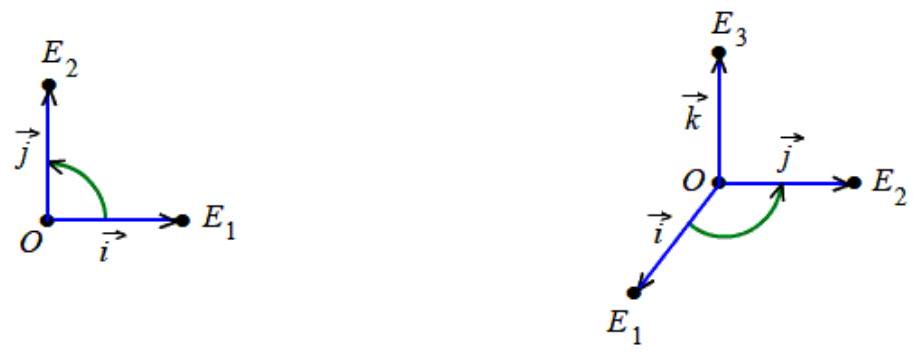
\includegraphics[max width=8cm, center]{2023_03_01_7659aec5e35f9a9b2d3cg-12(1)}

\item La referencia $\mathcal{C}=\{(1, \ldots, 0), \ldots,(0, \ldots, 1) ;(0, \ldots, 0)\}$ de $K^{n}$ se llama referencia canónica de $K^{n}$. Su base asociada es la base canónica $C=\left(e_{1}=(1, \ldots, 0), \ldots, e_{n}=(0, \ldots, 1)\right)$ de $K^{n}$.

\item $\{(1,2),(2,-1) ;(3,2)\}$ es una referencia de $\mathbb{R}^{2}$.
\end{enumerate}

\subsubsection{Definición - Coordenadas o coordenadas afines}
Sea $\mathbb{A}$ un espacio afín de dimensión $n$ y sea $\mathcal{R}=\left\{P_{1}, \ldots, P_{n} ; Q\right\}$ una referencia de $\mathbb{A}$. Se llaman coordenadas o coordenadas afines del punto $P \in \mathbb{A}$ en la referencia $\mathcal{R}$ a la $n$-pla $\left(x_{1}, \ldots, x_{n}\right)$ de coordenadas del vector $\overrightarrow{Q P}$ en la base $B_{\mathcal{R}}$, es decir a la $n$-pla $\left(x_{1}, \ldots, x_{n}\right) \in K^{n}$ tal que
$$
\overrightarrow{Q P}=\sum_{i=1}^{n} x_{i} \overrightarrow{Q P_{i}}
$$
\noindent El siguiente dibujo ilustra esta definición en el caso $n=2$.

\begin{center}
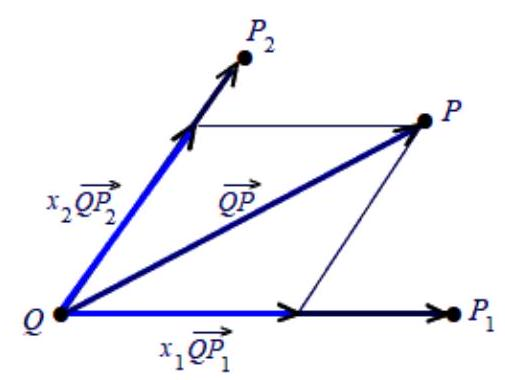
\includegraphics[max width=5cm]{2023_03_01_7659aec5e35f9a9b2d3cg-12(2)}
\end{center}

\ejemplos
\begin{enumerate}[label=(\arabic*)]
\item En la referencia canónica $\mathcal{C}$ de $K^{n}$, el punto $P=\left(x_{1}, \ldots, x_{n}\right)$ tiene coordenadas $\left(x_{1}, \ldots, x_{n}\right)$.

\item En la referencia $\mathcal{R}=\{(1,2),(2,-1) ;(3,2)\}$ de $\mathbb{R}^{2}$, el punto $P=(0,5)$ tiene coordenadas $(2,-1)$:
$$
2 \overrightarrow{QA} - \operatorname{QB} = (-4,0) + (1,3) = (-3,3) = (0,5) - (3,2) = \overrightarrow{QP}
$$
\end{enumerate}

\subsubsection{Definición - Punto medio}
Si la característica de $K$ es distinta de 2 , se llama punto medio de los puntos $P_{1}$ y $P_{2}$ al punto $M$ tal que $\overrightarrow{M P_{1}}=-\overrightarrow{M P_{2}}$.

\begin{center}
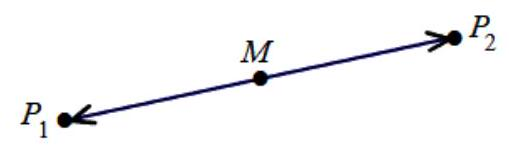
\includegraphics[max width=5cm]{2023_03_01_7659aec5e35f9a9b2d3cg-12}
\end{center}

\subsubsection{Lema - Condición equivalente al punto medio}
Si la característica de $K$ es distinta de 2 , entonces $M$ es el punto medio de $P_{1}$ y $P_{2}$ si, y solo si, $M=P_{1}+\frac{1}{2} \overrightarrow{P_{1} P_{2}}$ o, equivalentemente, si $M=P_{2}+\frac{1}{2} \overrightarrow{P_{2} P_{1}}$.

\demostracion

\noindent Se tiene:
$$
\begin{aligned}
\overrightarrow{M P_{1}}=-\overrightarrow{M P_{2}} & \Longleftrightarrow \overrightarrow{P_{1} M}=-\overrightarrow{P_{2} M} \Longleftrightarrow \overrightarrow{P_{1} M}=-\overrightarrow{P_{2} P_{1}}-\overrightarrow{P_{1} M} \\
& \Longleftrightarrow 2 \overrightarrow{P_{1} M}=\overrightarrow{P_{1} P_{2}} \Longleftrightarrow M=P_{1}+\frac{1}{2} \overrightarrow{P_{1} P_{2}} \\
& \Longleftrightarrow M=P_{2}+\overrightarrow{P_{2} P_{1}}-\frac{1}{2} \overrightarrow{P_{2} P_{1}} \\
& \Longleftrightarrow M=P_{2}+\frac{1}{2} \overrightarrow{P_{2} P_{1}}
\end{aligned}
$$
\observacion

$M$ es el punto medio de $P_1$ y $P_2 \Longleftrightarrow M = P_2 + \frac{1}{2} \overrightarrow{P_2 P_1}$. $M = P_1 + \frac{1}{2} \overrightarrow{P_1 P_2} \Longleftrightarrow M = P_2 + \overrightarrow{P_2 P_1} + \frac{1}{2} \overrightarrow{P_1 P_2} = P_2 - \overrightarrow{P_1 P_2} + \frac{1}{2} \overrightarrow{P_1 P_2} = -P_2 - \frac{1}{2} P_1 P_2 = P_2 + \frac{1}{2} P_2 P_1$.

\subsubsection{Lema - Propiedades de las coordenadas}
Sean $\mathbb{A}$ un espacio afín sobre el espacio vectorial $V, \mathcal{R}=\left\{P_{1}, \ldots, P_{n} ; Q\right\}$ una referencia de $\mathbb{A}$ y $B_{\mathcal{R}}=\left(v_{1}, \ldots, v_{n}\right)$.
\begin{enumerate}[label=(\arabic*)]
\item Si los puntos $P$ y $P'$ tienen coordenadas $\left(x_{1}, \ldots, x_{n}\right)$ y $\left(x_{1}^{\prime}, \ldots, x_{n}^{\prime}\right)$ en $\mathcal{R}$, respectivamente, entonces las coordenadas del vector $\overrightarrow{PP'}$ en $B_\mathcal{R}$ son $(x_1'-x_1,\ldots,x_n'-x_n)$.

\item Si el punto $P$ tiene coordenadas $\left(x_{1}, \ldots, x_{n}\right)$ en $\mathcal{R}$ y el vector $v$ tiene coordenadas $\left(z_{1}, \ldots, z_{n}\right)$ en $B_{\mathcal{R}}$, entonces las coordenadas del punto $P+v$ en $\mathcal{R}$ son $\left(x_{1}+z_{1}, \ldots, x_{n}+z_{n}\right)$.

\item Si los puntos $P$ y $P'$ tienen coordenadas $\left(x_{1}, \ldots, x_{n}\right)$ y $\left(x_{1}^{\prime}, \ldots, x_{n}^{\prime}\right)$ en $\mathcal{R}$, respectivamente, entonces las coordenadas del punto medio de $P$ y $P^{\prime}$ en $\mathcal{R}$ son $\frac{1}{2}\left(x_{1}+x_{1}^{\prime}, \ldots, x_{n}+x_{n}^{\prime}\right)$.
\end{enumerate}
\demostracion
\begin{enumerate}[label=(\arabic*)]
\item Se tiene
$$
\overrightarrow{Q P}=\sum_{i=1}^{n} x_{i} \overrightarrow{QP}, \quad \overrightarrow{Q P^{\prime}}=\sum_{i=1}^{n} x_{i}^{\prime} \overrightarrow{QP}, \quad \overrightarrow{P P^{\prime}}=\overrightarrow{P Q}+\overrightarrow{Q P^{\prime}}=\overrightarrow{Q P^{\prime}}-\overrightarrow{Q P}
$$
luego
$$
\overrightarrow{P P^{\prime}}=\sum_{i=1}^{n}\left(x_{i}^{\prime}-x_{i}\right) \overrightarrow{QP}
$$
\item Dado que
$$
\overrightarrow{Q P}=\sum_{i=1}^{n} x_{i} \overrightarrow{QP}, \quad v=\sum_{i=1}^{n} z_{i} \overrightarrow{QP}, \quad \overrightarrow{Q, P+v}=\overrightarrow{Q P}+\overrightarrow{P, P+v}=\overrightarrow{Q P}+v
$$
se tiene
$$
\overrightarrow{Q, P+v}=\sum_{i=1}^{n}\left(x_{i}+z_{i}\right) \overrightarrow{QP}
$$
\item $\displaystyle M = P_1 + \frac{1}{2}\overrightarrow{PP'}$.
\begin{gather*}
\overrightarrow{QM} = \overrightarrow{Q,P + \frac{1}{2}\overrightarrow{PP'}} = \overrightarrow{QP} \overrightarrow{P,P + \frac{1}{2}\overrightarrow{PP'}} = \overrightarrow{QP} \frac{1}{2}\overrightarrow{PP'} = \sum_{i=1}^{n} x_i \overrightarrow{QP_i} + \frac{1}{2} \sum_{i=1}^{n} (x_i' - x_i) \overrightarrow{QP_i} = \\
= \sum_{i=1}^{n} \left(\frac{x_i + x_i' - x_i}{2}\right) \overrightarrow{QP_i} = \sum_{i=1}^{n} \left(\frac{x_i + x_i'}{2}\right) \overrightarrow{QP_i}
\end{gather*}
\end{enumerate}

\subsubsection{Lema - Punto medio de dos puntos iguales}
Sea $\mathbb{A}$ un espacio afín sobre un $K$ espacio vectorial $V$, con característica distinta de $2$. Entonces, si $P_M(P_1,P_2)$ denota el punto medio de $P_1,P_2 \in \mathbb{A}$, se tiene que $P_M(P_1,P_2) = P_1 \Longleftrightarrow P_1 = P_2$. En particular, si $P_1 \neq P_2$, entonces $P_1 \neq P_M(P_2,P_2) \neq P_2$.

\demostracion
\dobleimplicacion{
	$\displaystyle P_M(P_1,P_2) = P_1 + \frac{1}{2} \overrightarrow{P_1 P_2} = P_1 + 0 \Longrightarrow \overrightarrow{P_1 P_2} = 0 \Longrightarrow P_1 = P_2$.
}{
	$\displaystyle P_1 = P_2 \Longleftrightarrow P_M(P_1,P_2) = P_1 + \frac{1}{2} \overrightarrow{P_1 P_2} = P_1$.
}

\subsubsection{Corolario - Mínimo de puntos de $\mathbb{A}$}
En las condiciones anteriores, si $\mathbb{A}$ es una recta, entonces $\mathbb{A}$ tiene al menos $3$ puntos distintos.

\demostracion

\noindent Sabemos que $\exists P_1, P_2 \in \mathbb{A}, P_1 \neq P_2$. Así, $P_3 = P_M(P_1 P_2) \,/\, P_1 \neq P_2 \neq P_3 \neq P_1$.

\ejemplo

\noindent $\mathbb{Z}_3$ es una recta y tiene $3$ puntos:
$$
\mathbb{Z}_3 = \{0,1,2\}, \quad P_M(0,1) = 2, \; P_M(1,2) = 0, \; P_M(2,0) = 1
$$

\subsubsection{Definición - Matriz de cambio de base}
\noindent Sean $B=\left(v_{1}, \ldots, v_{n}\right)$ y $B^{\prime}=\left(v_{1}^{\prime}, \ldots, v_{n}^{\prime}\right)$ bases de un espacio vectorial $V$ y sea
$$
\overrightarrow{QP}^{\prime}=\sum_{j=1}^{n} a_{j i} v_{j}, \quad i=1, \ldots, n
$$
La matriz
$$
\operatorname{Id}_{B^{\prime} B}=\left(\begin{array}{rrr}
	a_{11} & \ldots & a_{1 n} \\
	\vdots & \ddots & \vdots \\
	a_{n 1} & \ldots & a_{n n}
\end{array}\right)=\left(a_{i j}\right)
$$
se llama matriz de cambio de base de $B^{\prime}$ a $B$.

\subsubsection{Proposición}
Sean $L$ una variedad lineal de $\mathbb{A}, \mathcal{R}=\left\{P_{1}, \ldots, P_{n} ; Q\right\}$ una referencia de $\mathbb{A}$, $\mathcal{R}^{\prime}=\left(P_{1}^{\prime}, \ldots, P_{r}^{\prime} ; Q^{\prime}\right)$ una referencia de $L$. Supongamos que $\left(a_{1}, \ldots, a_{n}\right)$ son las coordenadas de $Q^{\prime}$ en $\mathcal{R}$ y que
$$
Q_{j}^{\prime} P_j'=\sum_{i=1}^{n} a_{i j} \overrightarrow{QP_{i}}, \quad j=1, \ldots, r
$$
\noindent Si $P$ es un punto de $L$ de coordenadas $\left(x_{1}, \ldots, x_{n}\right)$ en $\mathcal{R}$ y $\left(x_{1}^{\prime}, \ldots, x_{r}^{\prime}\right)$ en $\mathcal{R}^{\prime}$, entonces
$$
\left(\begin{array}{r}
x_{1} \\
\vdots \\
x_{n}
\end{array}\right)=\left(\begin{array}{r}
a_{1} \\
\vdots \\
a_{n}
\end{array}\right)+\left(\begin{array}{rll}
a_{11} & \ldots & a_{1 r} \\
\vdots & \ddots & \vdots \\
a_{n 1} & \ldots & a_{n r}
\end{array}\right)\left(\begin{array}{r}
x_{1}^{\prime} \\
\vdots \\
x_{r}^{\prime}
\end{array}\right)
$$
Esta expresión se denomina ecuación matricial del cambio de coordenadas de los puntos de $L$ de la referencia $\mathcal{R}^{\prime}$ a la referencia $\mathcal{R}$.

\begin{center}
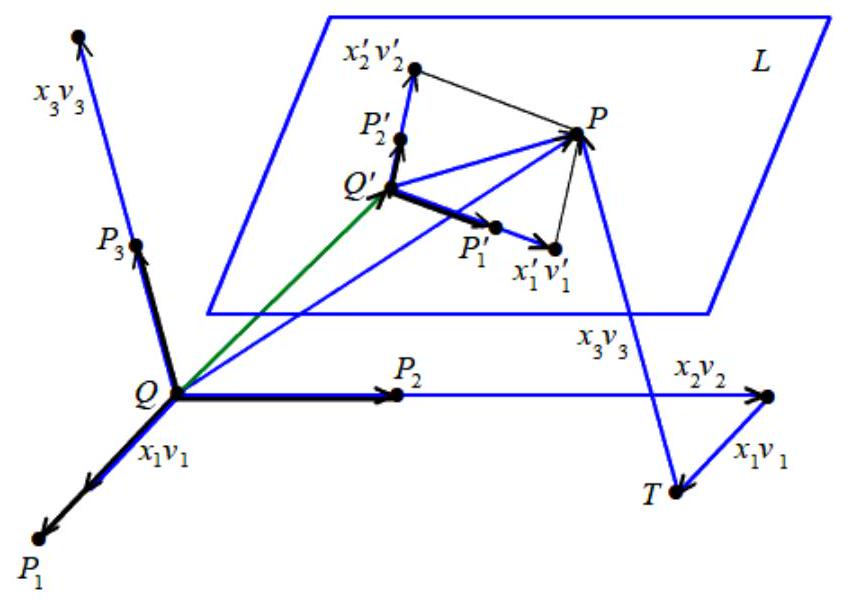
\includegraphics[max width=8cm]{2023_03_01_7659aec5e35f9a9b2d3cg-14}
\end{center}

\demostracion

\noindent Dado que $\overrightarrow{Q P}=\overrightarrow{Q Q^{\prime}}+\overrightarrow{Q^{\prime} P}$, se tiene

$$
\begin{aligned}
\sum_{i=1}^{n} x_{i} \overrightarrow{QP_i} & =\sum_{i=1}^{n} a_{i} \overrightarrow{QP_i}+\sum_{j=1}^{r} x_{j}^{\prime} v_{j}^{\prime}=\sum_{i=1}^{n} a_{i} \overrightarrow{QP_i}+\sum_{j=1}^{n} x_{j}^{\prime}\left(\sum_{i=1}^{n} a_{i j} \overrightarrow{QP_i}\right) \\
& =\sum_{i=1}^{n} a_{i} \overrightarrow{QP_i}+\sum_{i=1}^{n}\left(\sum_{j=1}^{r} a_{i j} x_{j}^{\prime}\right) \overrightarrow{QP_i}
\end{aligned}
$$
\noindent de donde se sigue
$$
x_{i}=a_{i}+\sum_{j=1}^{r} a_{i j} x_{j}^{\prime}, \quad i=1, \ldots, n \text {. }
$$

\subsubsection{Teorema - Cambio de coordenadas.}
Sean $\mathcal{R}=\left\{P_{1}, \ldots, P_{n} ; Q\right\}$ y $\mathcal{R}^{\prime}=\left\{P_{1}^{\prime}, \ldots, P_{n}^{\prime} ; Q^{\prime}\right\}$ referencias de $\mathbb{A}$. Sea $P$ un punto de coordenadas $\left(x_{1}, \ldots, x_{n}\right)$ en la referencia $\mathcal{R}$ y coordenadas $\left(x_{1}^{\prime}, \ldots, x_{n}^{\prime}\right)$ en la referencia $\mathcal{R}^{\prime}$. Si $\left(\operatorname{Id}_{B_{\mathcal{R}^{\prime}} B_{\mathcal{R}}}\right)=\left(a_{i j}\right)$ es la matriz de cambio de base de $B_{\mathcal{R}^{\prime}}$ a $B_{\mathcal{R}}$, entonces

$$
\left(\begin{array}{c}
x_{1} \\
\vdots \\
x_{n}
\end{array}\right)=\left(\begin{array}{c}
b_{1} \\
\vdots \\
b_{n}
\end{array}\right)+\left(\operatorname{Id}_{B_{\mathcal{R}^{\prime}} B_{\mathcal{R}}}\right)\left(\begin{array}{c}
x_{1}^{\prime} \\
\vdots \\
x_{n}^{\prime}
\end{array}\right),
$$

donde $\left(b_{1}, \ldots, b_{n}\right)$ son las coordenadas de $Q^{\prime}$ en $\mathcal{R}$. Esta ecuación se llama ecuación matricial del cambio de coordenadas de $\mathcal{R}^{\prime}$ a $\mathcal{R}$.

\demostracion

\noindent Es un caso particular de la proposición anterior, basta tomar $L=\mathbb{A}$.

\subsection{Ecuaciones de las variedades lineales}

\subsubsection{Proposición - Variedad lineal dada por un sistema de ecuaciones lineales}
Sea $\mathcal{R}=\left\{P_{1}, \ldots, P_{n} ; Q\right\}$ una referencia de $\mathbb{A}$ sobre un $K$ espacio vectorial. Sea $C = (c_{ij}) \in \mathcal{M}_{m \times n}(K)$ y $(d_1,\ldots,d_n) \in K^m$. El conjunto $S$ de puntos de $\mathbb{A}$ cuyas coordenadas $\left(x_{1}, \ldots, x_{n}\right)$ en $\mathcal{R}$ son solución del sistema de ecuaciones lineales
$$
\begin{aligned}
c_{11} x_{1}+\ldots+c_{1 n} x_{n}= & d_{1} \\
c_{21} x_{1}+\ldots+c_{2 n} x_{n}= & d_{2} \\
\vdots & \vdots \\
c_{m 1} x_{1}+\ldots+c_{m n} x_{n}= & d_{m}
\end{aligned}
$$
es una variedad lineal de $\mathbb{A}$. Además, si $S \neq \varnothing$, entonces la dimensión de $S$ es $n$ - rango $\left(c_{i j}\right)$ y los vectores de la dirección de $S$ son los vectores cuyas coordenadas en $B_{\mathcal{R}}$ son solución del sistema de ecuaciones lineales homogéneo asociado al anterior.

\demostracion

\noindent Si $S = \varnothing$, acabamos. Supongamos que $S \neq \varnothing$. Sea $B_\mathcal{R} = \left(\overrightarrow{QP_1},\ldots,\overrightarrow{QP_n}\right) = (v_1,\ldots,v_n)$. Sea $f: V \rightarrow K^{m}$ la aplicación lineal definida por
$$
f\left(v_{i}\right)=\left(c_{1 i}, \ldots, c_{m i}\right), \quad i=1, \ldots, n
$$
Entonces,
$$
f\left(\sum_{i=1}^{n} x_{i} v_{i}\right)=\sum_{i=1}^{n}x_if(v_i)=\sum_{i=1}^{n}x_i(c_{1i},\ldots,c_{mi})=\left(\sum_{i=1}^{n} c_{1 i} x_{i}, \ldots, \sum_{i=1}^{n} c_{m i} x_{i}\right) .
$$
Si $P$ es el punto de coordenadas $\left(x_{1}, \ldots, x_{n}\right)$ en $\mathcal{R}$, se tiene
$$
P \in S \Longleftrightarrow \sum_{i=1}^{n} c_{j i} x_{i}=d_{j}, j=1, \ldots, m \Longleftrightarrow\left(\sum_{i=1}^{n} c_{1 i} x_{i}, \ldots, \sum_{i=1}^{n} c_{m i} x_{i}\right)=\left(d_{1}, \ldots, d_{m}\right),
$$
Nótese que $\displaystyle \overrightarrow{QP} = \sum_{i=1}^{n} x_i v_i$. Así, $P \in S$ si, y sólo si, $f(\overrightarrow{Q P})=\left(d_{1}, \ldots, d_{m}\right)$. Si $A \in S$, entonces $S=A+\ker f$, donde $\ker f=\{v \in V \mid f(v)=0\} ;$ en efecto,
$$
P \in S \Longleftrightarrow f(\overrightarrow{Q P})=\left(d_{1}, \ldots, d_{m}\right)=f(\overrightarrow{Q A}) \Longleftrightarrow \overrightarrow{Q P}-\overrightarrow{Q A} \in \ker f \Longleftrightarrow \overrightarrow{A P} \in \ker f \Longleftrightarrow P \in A+\ker f
$$
Por tanto,
$$
\dim  S=\dim _{K} \ker f=n-\dim _{K} f(V)=n-\operatorname{rango}\left(c_{i j}\right) .
$$
\noindent Además, un vector de coordenadas $\left(x_{1}, \ldots, x_{n}\right)$ en $B_{\mathcal{R}}$ está en la dirección de $S$, si, y solo si,
$$
f\left(\sum_{i=1}^{n} x_{i} v_{i}\right)=(0, \ldots, 0) \Longleftrightarrow\left(\sum_{i=1}^{n} c_{1 i} x_{i}, \ldots, \sum_{i=1}^{n} c_{m i} x_{i}\right)=(0, \ldots, 0),
$$
\noindent de donde se sigue que unas ecuaciones en la base $B_{\mathcal{R}}$ del subespacio dirección de $S$ son
$$
\sum_{i=1}^{n} c_{j i} x_{i}=0, \quad j=1, \ldots, m
$$

\subsubsection{Proposición - Ecuaciones paramétricas de una variedad lineal}
Sean $L=A+U$ una variedad lineal de $\mathbb{A}, \mathcal{R}=\left\{P_{1}, \ldots, P_{n} ; Q\right\}$ una referencia de $\mathbb{A}, B_{\mathcal{R}}=\left(v_{1}, \ldots, v_{n}\right)$ y $B_{U}=\left\{u_{1}, \ldots, u_{r}\right\}$ una base de $U$. Supongamos que $\left(a_{1}, \ldots, a_{n}\right)$ son las coordenadas de $A$ en $\mathcal{R}$ y que
$$
u_{j}=\sum_{i=1}^{n} a_{i j} v_{i}, \quad j=1, \ldots, r
$$
\noindent Si $P$ es un punto de $L$ de coordenadas $\left(x_{1}, \ldots, x_{n}\right)$ en $\mathcal{R}$, entonces
$$
P \in L \Longleftrightarrow \exists \lambda_{1}, \ldots, \lambda_{r} \in K \mid x_{i}=a_{i}+\sum_{j=1}^{r} \lambda_{j} a_{i j}, \quad i=1, \ldots, n
$$
\noindent Los escalares $\lambda_{1}, \ldots, \lambda_{r}$ se llaman parámetros.

\demostracion 

Se tiene que $P \in L$ si, y solo si, existe $u \in U$ tal que $P=A+u$, equivalentemente si existen escalares $\lambda_{1}, \ldots, \lambda_{r} \in K$ tales que
$$
P=A+\sum_{j=1}^{r} \lambda_{j} u_{j}
$$
\noindent Se tiene
$$
P \in L \Longleftrightarrow \exists \lambda_{1}, \ldots, \lambda_{r} \in K \mid\left(x_{1}, \ldots, x_{n}\right)=\left(a_{1}, \ldots, a_{n}\right)+\lambda_{1}\left(a_{11}, \ldots, a_{r 1}\right)+\ldots+\lambda_{r}\left(a_{1 r}, \ldots, a_{n r}\right),
$$
y el resultado se sigue igualando coordenadas.

\ejemplo

Unas ecuaciones paramétricas del plano $\Pi=(0,1,1)+\langle(1,1,1),(1,0,2)\rangle$ de $\mathbb{R}^{3}$ en la referencia canónica están dadas por
$$
(x, y, z) \in \Pi \Longleftrightarrow\left\{\begin{array}{l}
x=\lambda_{1}+\lambda_{2} \\
y=1+\lambda_{1} \\
z=1+\lambda+2 \lambda_{2}
\end{array}\right.
$$
donde $\lambda_{1}, \lambda_{2} \in \mathbb{R}$. Para calcular unas ecuaciones paramétricas del plano $\Pi$ en la referencia
$$
\mathcal{R}=\{(1,-1,0),(0,1,0),(0,1,1) ;(1,1,1)\}
$$
obtenemos que las coordenadas del punto $(0,1,1)$ en $\mathcal{R}$ son $(0,0,1)$, las coordenadas del vector $(1,1,1)$ en $B_{\mathcal{R}}=\{(0,-2,-1),(-1,0,-1),(-1,0,0)\}$ son $(-1 / 2,-1 / 2,-1 / 2)$ y las coordenadas del vector $(1,0,2)$ en $B_{\mathcal{R}}$ son $(0,-2,1)$. Si $P$ es el punto de coordenadas $\left(x^{\prime}, y^{\prime}, z^{\prime}\right)$ en $\mathcal{R}$, entonces
$$
P \in \Pi \Longleftrightarrow\left\{\begin{array}{l}
x^{\prime}=-(1 / 2) \lambda_{1} \\
y^{\prime}=-(1 / 2) \lambda_{1}-2 \lambda_{2} \\
z^{\prime}=1-(1 / 2) \lambda_{1}+\lambda_{2}
\end{array}\right.
$$
donde $\lambda_{1}, \lambda_{2} \in \mathbb{R}$, con lo que se tienen unas ecuaciones paramétricas de $\Pi$ en $\mathcal{R}$.

\noindent\underline{Otro método}

Si $P \in H$ tiene coordenadas $(x',y',z')$ en $\mathcal{R}$ y coordenadas $(x,y,z,t)$ en $\mathbb{R}^4$ con $\mathcal{C}$: Cambio de referencia de $\mathcal{R}$ a $\mathcal{C}$
$$
\begin{pmatrix}
	x \\
	y \\
	z \\
	t
\end{pmatrix} = \begin{pmatrix}
	0 \\
	1 \\
	0 \\
	1 \\ 
\end{pmatrix} + \begin{pmatrix}
	1 & 0 & 0 \\
	0 & 0 & -1 \\
	0 & 1 & 1 \\
	-1 & -1 & 0
\end{pmatrix} \begin{pmatrix}
	x' \\
	y' \\
	z'
\end{pmatrix}
$$
Así,
$$
\left. \begin{array}{r}
	x = x' \\
	y = 1 - z' \\
	z = y' + z'
\end{array} \right\} \Longrightarrow t = 1 - x' - y'
$$
son las coordenadas de $B_\mathcal{R}$ en $\mathcal{C}$.

\subsubsection{Proposición - Ecuaciones lineales o implícitas de una variedad lineal}
Sean $L=A+U$ una variedad lineal de $\mathbb{A}$ de dimensión $r, \mathcal{R}=\left\{P_{1}, \ldots, P_{n} ; Q\right\}$ una referencia de $\mathbb{A}, B_{\mathcal{R}}=\left(v_{1}, \ldots, v_{n}\right) \mathrm{y}$ $B_{U}=\left\{u_{1}, \ldots, u_{r}\right\}$ una base de $U$. Supongamos que $\left(a_{1}, \ldots, a_{n}\right)$ son las coordenadas de $A$ en $\mathcal{R}$ y que
$$
u_{j}=\sum_{i=1}^{n} a_{i j} v_{i}, \quad j=1, \ldots, r .
$$
\noindent Si $P$ es un punto de $L$ de coordenadas $\left(x_{1}, \ldots, x_{n}\right)$ en $\mathcal{R}$, se tiene
$$
P \in L \Longleftrightarrow \operatorname{rango}\left(\begin{array}{cccc}
x_{1}-a_{1} & a_{11} & \cdots & a_{1 r} \\
\vdots & \vdots & \ddots & \vdots \\
x_{n}-a_{n} & a_{n 1} & \cdots & a_{n r}
\end{array}\right)=r .
$$
\noindent En particular, si
$$
\Delta=\left|\begin{array}{ccc}
a_{11} & \ldots & a_{1 r} \\
\vdots & \ddots & \vdots \\
a_{r 1} & \ldots & a_{r r}
\end{array}\right| \neq 0
$$
\noindent entonces
$$
P \in L \Longleftrightarrow\left|\begin{array}{rrrr}
x_{1}-a_{1} & a_{11} & \ldots & a_{1 r} \\
\vdots & \vdots & \ddots & \vdots \\
x_{r}-a_{r} & a_{r 1} & \ldots & a_{r r} \\
x_{j}-a_{j} & a_{j 1} & \ldots & a_{j r}
\end{array}\right|=0, \quad j=r+1, \ldots, n .
$$
\noindent Así, toda variedad lineal de dimensión $r$ en un espacio afín de dimensión $n$ queda determinada por el conjunto de soluciones de un sistema de $n-r$ ecuaciones lineales y $n$ incógnitas, donde el rango de la matriz de coeficientes es $n-r$. Por la proposición 1.2.15, unas ecuaciones del subespacio dirección $U$ de $L$ en la base $B_{\mathcal{R}}$ están dadas por el sistema de ecuaciones lineales homogéneo asociado al sistema de ecuaciones lineales de $L$ en $\mathcal{R}$.

\demostracion

\noindent Se tiene que $P \in L$ si, y solo si, $\overrightarrow{A P} \in U$, es decir,
$$
P \in L \Longleftrightarrow \overrightarrow{A Q}+\overrightarrow{Q P} \in U \Longleftrightarrow \sum_{i=1}^{n}\left(x_{i}-a_{i}\right) v_{i} \in\left\langle\sum_{i=1}^{n} a_{i 1} v_{i}, \ldots, \sum_{i=1}^{n} a_{i r} v_{i}\right\rangle
$$
\noindent luego
$$
P \in L \Longleftrightarrow \operatorname{rango}\left(\begin{array}{cccc}
x_{1}-a_{1} & a_{11} & \cdots & a_{1 r} \\
\vdots & \vdots & \ddots & \vdots \\
x_{n}-a_{n} & a_{n 1} & \cdots & a_{n r}
\end{array}\right)=r
$$
\observacion

Sea $\mathbb{A}$ un espacio afín de dimensión $n$ y $L$ una variedad lineal de $\mathbb{A}$ de dimensión $r$. El menor número de ecuaciones lineales de un sistema de ecuaciones lineales de $L$ es $n-r$. En efecto, las coordenadas de los puntos de $L$ son el conjunto de soluciones de un sistema de $n-r$ ecuaciones lineales y $n$ incógnitas. Si las coordenadas de los puntos de $L$ fuesen el conjunto de soluciones de un sistema de $m<n-r$ ecuaciones lineales y $n$ incógnitas y $\mathcal{A}$ es la matriz de coeficientes de este sistema, entonces por la proposición 1.2.15, $\dim  L=n-\operatorname{rango} \mathcal{A} \geq n-m>n-(n-r)=r$.

\ejemplo

Una ecuación lineal del plano $\Pi=(0,1,1)+\langle(1,1,1),(1,0,2)\rangle$ en la referencia canónica se obtiene de la siguiente forma:
\begin{gather*}
(x, y, z) \in \Pi \Longleftrightarrow \operatorname{rango}\left(\begin{array}{ccc}x & 1 & 1 \\ y-1 & 1 & 0 \\ z-1 & 1 & 2\end{array}\right)=\dim  \Pi=2 \Longleftrightarrow \\ \Longleftrightarrow \left|\begin{array}{ccc}x & 1 & 1 \\ y-1 & 1 & 0 \\ z-1 & 1 & 2\end{array}\right|=0 \Longleftrightarrow 2 x-y-z+2=0
\end{gather*}
Sea $P$ el punto de coordenadas $\left(x^{\prime}, y^{\prime}, z^{\prime}\right)$ en la referencia $\mathcal{R}=\{(1,-1,0),(0,1,0),(0,1,1) ;(1,1,1)\}$. Una ecuación lineal del plano $\Pi$ en $\mathcal{R}$ se obtiene de la siguiente forma:
$$
P \in \Pi \Longleftrightarrow\left|\begin{array}{ccr}
x^{\prime} & -1 / 2 & 0 \\
y^{\prime} & -1 / 2 & -2 \\
z^{\prime}-1 & -1 / 2 & 1
\end{array}\right|=0 \Longleftrightarrow 3 x^{\prime}-y^{\prime}-2 z^{\prime}+2=0 .
$$

También se puede calcular una ecuación lineal de $\Pi$ en $\mathcal{R}$ a partir de su ecuación lineal en la referencia canónica y de las ecuaciones del cambio de coordenadas de la referencia $\mathcal{R}$ a la referencia canónica $(1.2 .14)$.

\ejemplo

Sea $H$ el hiperplano de $\mathbb{R}^{4}$ cuya ecuación en la referencia canónica es $x+y+z+t=2$. Sea $L$ la recta de $\mathbb{R}^{4}$ cuyas ecuaciones en la referencia canónica son
$$
L \equiv\left\{\begin{array}{l}
x-y=2 \\
2 x+z=4 \\
t=0
\end{array}\right.
$$
Se tiene que $L \subset H$ y que los puntos $(1,1,0,0),(0,1,1,0),(0,0,1,1)$ y $(0,1,0,1)$ son puntos de $H$ afínmente independientes. Vamos a calcular unas ecuaciones lineales de la recta $L$ en la referencia
$$
\mathcal{R}=\{(1,1,0,0),(0,1,1,0),(0,0,1,1) ;(0,1,0,1)\}
$$
de $H$. Las coordenadas del punto $(0,-2,4,0)$ de $L$ en $\mathcal{R}$ son $(0,1,3)$ y las coordenadas del vector $(1,1,-2,0)$ de la dirección de $L$ en la base $B_{\mathcal{R}}=\{(1,0,0,-1),(0,0,1,-1),(0,-1,1,0)\}$ son $(1,-1,-1)$. Si $P$ es el punto de coordenadas $\left(x^{\prime}, y^{\prime}, z^{\prime}\right)$ en $\mathcal{R}$, entonces

$$
P \in L \Longleftrightarrow \operatorname{rango}\left(\begin{array}{cc}
x^{\prime} & 1 \\
y^{\prime}-1 & -1 \\
z^{\prime}-3 & -1
\end{array}\right)=1 \Longleftrightarrow\left|\begin{array}{cr}
x^{\prime} & 1 \\
y^{\prime}-1 & -1
\end{array}\right|=0,\left|\begin{array}{cr}
x^{\prime} & 1 \\
z^{\prime}-3 & -1
\end{array}\right|=0,
$$

luego

$$
P \in L \Longleftrightarrow L \equiv\left\{\begin{array}{l}
x^{\prime}+y^{\prime}-1=0 \\
x^{\prime}+z^{\prime}-3=0
\end{array}\right.
$$

También se pueden calcular unas ecuaciones lineales de $L$ en $\mathcal{R}$ a partir de las ecuaciones de $L$ en la referencia canónica y de las ecuaciones del cambio de coordenadas de la referencia $\mathcal{R}$ de $H$ a la referencia canónica (proposición 1.2.13). Obsérvese que 3 el número mínimo de ecuaciones lineales de $L$ como variedad lineal de $\mathbb{R}^{4}$ y que 2 es el número mínimo de ecuaciones lineales de $L$ como variedad lineal de $H$.

\subsubsection{Definición - Paralelogramo}
Sea $\mathbb{A}$ un espacio afín sobre el espacio vectorial $V$. Sean $P_{1}, P_{2}, P_{3}$ y $P_{4}$ cuatro puntos distintos y $l_{1}, l_{2}, l_{3}$ y $l_{4}$ cuatro rectas distintas. Se dice que los puntos $P_{1}, P_{2}, P_{3}, P_{4}$ son los vértices del paralelogramo de lados $l_{1}, l_{2}, l_{3}, l_{4}$ si se verifican las siguientes condiciones:
\begin{enumerate}[label=(\arabic*)]
\item $l_{1}\left\|l_{3}, l_{2}\right\| l_{4}$.

\item $l_{1} \cap l_{4}=\left\{P_{1}\right\}, l_{1} \cap l_{2}=\left\{P_{2}\right\}, l_{2} \cap l_{3}=\left\{P_{3}\right\}, l_{3} \cap l_{4}=\left\{P_{4}\right\}$.
\end{enumerate}
\begin{center}
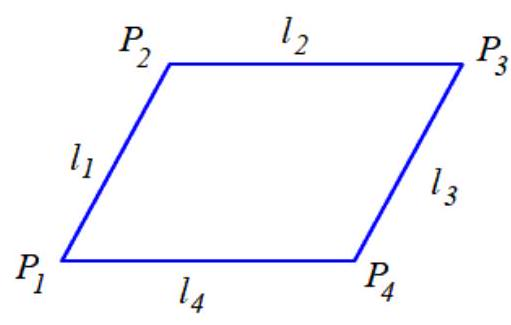
\includegraphics[max width=6cm]{2023_03_01_7659aec5e35f9a9b2d3cg-19}
\end{center}

Las longitudes de los lados opuestos de un paralelogramo se pueden comparar, ya que los lados opuestos de un paralelogramo son paralelos. La siguiente proposición demuestra que los lados opuestos de un paralelogramo tienen la misma longitud.

\subsubsection{Lema - Regla del paralelogramo}
Sean $P_{1}, P_{2}, P_{3}, P_{4}$ los vértices de un paralelogramo. Se tiene
$$
\overrightarrow{P_{1} P_{2}}=\overrightarrow{P_{4} P_{3}}, \quad \overrightarrow{P_{1} P_{4}}=\overrightarrow{P_{2} P_{3}}
$$
\demostracion

Dado que $P_{1} \circ P_{2} \| P_{4} \circ P_{3}$ y $P_{1} \circ P_{4} \| P_{2} \circ P_{4}$, existen escalares $a, b \in K$ tales que $\overrightarrow{P_{1} P_{2}}=a \overrightarrow{P_{4} P_{3}}$ y $\overrightarrow{P_{1} P_{4}}=b \overrightarrow{P_{2} P_{3}}$. Veamos que $a=b=1$. Por la relación de Chasles,
$$
\overrightarrow{P_{1} P_{2}}+\overrightarrow{P_{2} P_{3}}=\overrightarrow{P_{1} P_{3}}=\overrightarrow{P_{1} P_{4}}+\overrightarrow{P_{4} P_{3}}
$$
y por lo tanto
$$
a \overrightarrow{P_{4} P_{3}}+\overrightarrow{P_{2} P_{3}}=b \overrightarrow{P_{2}, P_{3}}+\overrightarrow{P_{4} P_{3}}
$$
de donde se sigue
$$
(a-1) \overrightarrow{P_{4} P_{3}}+(1-b) \overrightarrow{P_{2} P_{3}}=0
$$
Dado que $l_{2} \cap l_{3}=\left\{P_{3}\right\}$, los vectores $\overrightarrow{P_{4} P_{3}}$ y $\overrightarrow{P_{2} P_{3}}$ son linealmente independientes, luego $a=b=1$.

\subsection{Aplicaciones afines y grupo afín}
En esta sección consideraremos espacios vectoriales sobre un mismo cuerpo $K$. Si $K=\mathbb{Q}$ o $K=\mathbb{R}$, el teorema fundamental de la geometría afín [14] afirma que las afinidades de un espacio afín de dimensión finita $n \geq 2$ sobre un espacio vectorial son las aplicaciones biyectivas que llevan puntos alineados en puntos alineados. En esta sección damos la definición algebraica de afinidad y estudiamos sus propiedades algebraicas y geométricas; entre las afinidades de un espacio afín destacan las traslaciones y las homotecias que en espacios afines de dimensión $n \geq 2$ son las aplicaciones biyectivas que llevan cada recta en una recta paralela.

\subsubsection{Definición - Aplicación afín}
Sean $V$ y $V^{\prime}$ $K$-espacios vectoriales, $\mathbb{A}$ y $\mathbb{A}^{\prime}$ espacios afines sobre $V$ y $V^{\prime}$, respectivamente, y $O$ un punto de $\mathbb{A}$. Se dice que una aplicación $\alpha: \mathbb{A} \rightarrow \mathbb{A}^{\prime}$ es afín si la aplicación $\vec{\alpha}: V \rightarrow V^{\prime}$ definida como

$$
\vec{\alpha}(v)=\overrightarrow{\alpha(O), \alpha(O+v)}, \quad v \in V
$$

\noindent es una aplicación lineal.

\subsubsection{Lema - Independencia del origen y unicidad de $\overrightarrow{\alpha}$}
\noindent (Independencia del origen y unicidad de $\overrightarrow{\alpha}$). Si $\alpha: \mathbb{A} \rightarrow \mathbb{A}^{\prime}$ es una aplicación afín, entonces
$$
\vec{\alpha}(v)=\overrightarrow{\alpha(P), \alpha(P+v)}, \quad v \in V
$$
para cada $P \in \mathbb{A}$.

\demostracion

\noindent Se tiene
\begin{gather*}
\overrightarrow{\alpha(P), \alpha(P+v)} =\overrightarrow{\alpha(O+\overrightarrow{O P}), \alpha(O+\overrightarrow{O P}+v)}=\\\overrightarrow{\alpha(O+\overrightarrow{O P}), \alpha(O)}+\overline{\alpha(O), \alpha(O+\overrightarrow{O P}+v)} = \\ =-\vec{\alpha}(\overrightarrow{O P})+\vec{\alpha}(\overrightarrow{O P}+v)=\vec{\alpha}(v).
\end{gather*}


\subsubsection{Definición - Aplicación lineal asociada} Si $\alpha: \mathbb{A} \rightarrow \mathbb{A}^{\prime}$ es una aplicación afín, la aplicación lineal $\vec{\alpha}: V \rightarrow V^{\prime}$ se llama la aplicación lineal asociada a $\alpha$.

Se dice que la aplicación afín $\alpha: \mathbb{A} \rightarrow \mathbb{A}^{\prime}$ es un isomorfismo de espacios afines o afinidad si existe una aplicación afín $\beta: \mathbb{A}^{\prime} \rightarrow \mathbb{A}$ tal que $\beta \circ \alpha=\operatorname{id}_{\mathbb{A}}$ y $\alpha \circ \beta=\mathrm{id}_{\mathbb{A}^{\prime}}$ ($\beta$ es única y se denota $\alpha^{-1}$. Se denomina inversa de $\alpha$); los isomorfismos de espacios afines se llaman afinidades. Se dice que los espacios afines $\mathbb{A}$ y $\mathbb{A}^{\prime}$ son isomorfos si existe una afinidad $\alpha: \mathbb{A} \rightarrow \mathbb{A}^{\prime}$.\\

\subsubsection{Lema - Propiedad de $\overrightarrow{\alpha}$}
\noindent Si $\alpha: \mathbb{A} \rightarrow \mathbb{A}^{\prime}$ es una aplicación afín, entonces $\overrightarrow{\alpha(P), \alpha(Q)}=\vec{\alpha}(\overrightarrow{P Q})$, para todo $P, Q \in \mathbb{A}$.

\demostracion

\noindent Si $v=\overrightarrow{P Q}$, se tiene $\vec{\alpha}(\overrightarrow{P Q})=\overrightarrow{\alpha(P), \alpha(P+\overrightarrow{P Q})}=\overrightarrow{\alpha(P), \alpha(Q)}$.\\

\subsubsection{Proposición - Propiedades de las aplicaciones afines}
\noindent Sean $\mathbb{A}$ y $\mathbb{A}^{\prime}$ espacios afines sobre los espacios vectoriales $V$ y $V^{\prime}$, respectivamente.
\begin{enumerate}[label=(\arabic*)]
\item Si $A$ es un punto de $\mathbb{A}, A^{\prime}$ un punto de $\mathbb{A}^{\prime}$ y $f: V \rightarrow V^{\prime}$ una aplicación lineal, entonces la aplicación $\alpha: \mathbb{A} \rightarrow \mathbb{A}^{\prime}$ dada por $\alpha(P)=A^{\prime}+f(\overrightarrow{A P})$ es una aplicación afín cuya aplicación lineal asociada es $f$, y además $\alpha(A) = A^{'}$.

\item Si $\alpha: \mathbb{A} \rightarrow \mathbb{A}^{\prime}$ es una aplicación afín y $A \in \mathbb{A}$, entonces $\alpha(P)=\alpha(A)+\vec{\alpha}(\overrightarrow{A P})$, para cada $P \in \mathbb{A}$.

\item Toda aplicación afín $\alpha: \mathbb{A} \rightarrow \mathbb{A}^{\prime}$ está determinada conocida la imagen de un punto y su aplicación lineal asociada.
\end{enumerate}
\demostracion
\begin{enumerate}[label=(\arabic*)]
\item La aplicación $\alpha: \mathbb{A} \rightarrow \mathbb{A}^{\prime}$ dada por $\alpha(P)=A^{\prime}+f(\overrightarrow{A P})$ es una aplicación afín. En efecto, para cada $v \in V$,
$$
\vec{\alpha}(v)=\overrightarrow{\alpha(P), \alpha(P+v)}=\overrightarrow{A^{\prime}+f(\overrightarrow{A P}), A^{\prime}+f(\overrightarrow{A, P+v})}=-f(\overrightarrow{A P})+f(\overrightarrow{A, P+v})=f(\overrightarrow{PA}+\overrightarrow{A,P+v})=f(\overrightarrow{P, P+v})=f(v)
$$

\item Dado que $\overrightarrow{\alpha(A), \alpha(P)}=\vec{\alpha}(\overrightarrow{A P})$, se tiene que $\alpha(P)=\alpha(A)+\vec{\alpha}(\overrightarrow{A P})$.

\item Se sigue de (2).
\end{enumerate}
\ejemplo

La aplicación afín $\alpha: \mathbb{R}^{3} \rightarrow \mathbb{R}^{4}$ tal que $\alpha(1,0,1)=(2,-1,1,0)$ y cuya aplicación lineal asociada es $\vec{\alpha}: \mathbb{R}^{3} \rightarrow \mathbb{R}^{4}, \vec{\alpha}(x, y, z)=(x, 2 y-z, 0, x+y+z)$, es la aplicación dada por
\begin{gather*}
\alpha(x, y, z) =(2,-1,1,0)+\vec{\alpha}(x-1, y, z-1)=(2,-1,1,0)+\\+(x-1,2 y-z+1,0, x+y+z-2) =(1+x, 2 y-z, 1,-2+x+y+z).
\end{gather*}

\subsubsection{Proposición - Más propiedades de las aplicaciones afines}
\begin{enumerate}[label=(\arabic*)]
\item Si $\alpha: \mathbb{A}_{1} \rightarrow \mathbb{A}_{2}$ y $\beta: \mathbb{A}_{2} \rightarrow \mathbb{A}_{3}$ son aplicaciones afines, entonces $\beta \circ \alpha$ es una aplicación afín con $\overrightarrow{\alpha_{2}\circ\alpha_{1}}=\overrightarrow{\alpha_{2}}\circ\overrightarrow{\alpha_{1}}$.

\item $\operatorname{Id}_{\mathbb{A}}: \mathbb{A} \rightarrow \mathbb{A}$ es una aplicación afín con $\overrightarrow{\operatorname{Id}_{\mathbb{A}}}=\operatorname{Id_{V}}$.

\item Si $\alpha$ es una afinidad, entonces $\alpha^{-1}$ también es una afinidad.

\item El conjunto

$$
G(\mathbb{A})=\{\alpha: \mathbb{A} \rightarrow \mathbb{A} \mid \alpha \text { afinidad }\}
$$

es un grupo con la operación composición.
\end{enumerate}

\demostracion
\begin{enumerate}[label=(\arabic*)]
\item Para cada $v \in V$,

\begin{gather*}
(\overrightarrow{\beta \circ \alpha})(v)=\overrightarrow{(\beta \circ \alpha)(P),(\beta \circ \alpha)(P+v)})=\overrightarrow{\beta(\alpha(P)), \beta(\alpha(P)+\vec{\alpha}(v))}=\\=\vec{\beta}(\vec{\alpha}(v))=(\vec{\beta} \circ \vec{\alpha})(v),
\end{gather*}

luego $\overrightarrow{\beta \circ \alpha}=\vec{\beta} \circ \vec{\alpha}$ es una aplicación lineal.

\item La aplicación identidad $\operatorname{id}_{\mathbb{A}}: \mathbb{A} \rightarrow \mathbb{A}$, $\operatorname{id}_{\mathbb{A}}(P)=P$ para cada $P \in P$, es una aplicación afín con aplicación lineal asociada $\mathrm{id}_{V}$.

\item Simetría en la definición de isomorfismo.

\item Se sigue de (1) y (2).

El grupo $(G(\mathbb{A}), \circ)$ se llama grupo afín de $\mathbb{A}$ y se denota simplemente por $G(\mathbb{A})$.
\end{enumerate}

\subsubsection{Proposición - Condiciones equivalentes a afinidad}
	\noindent Sea $\alpha: \mathbb{A} \rightarrow \mathbb{A}^{\prime}$ una aplicación afín. Son equivalentes:
	\begin{enumerate}[label=(\arabic*)]
		\item $\alpha$ es una afinidad,
		
		\item $\alpha$ es una aplicación biyectiva,
		
		\item $\vec{\alpha}$ es un isomorfismo de espacios vectoriales.
	\end{enumerate}

\demostracion 
	\begin{itemize}
		\item$(1) \Rightarrow(2)$ Trivial.
		
		\item$(2) \Rightarrow(3)$ Veamos que $\vec{\alpha}$ es inyectiva. Sea $v \in V$ tal que $\vec{\alpha}(v)=0$. Se tiene
		
		$$
		\overrightarrow{\alpha(P), \alpha(P+v)}=\vec{\alpha}(\overrightarrow{P, P+v})=\vec{\alpha}(v)=0
		$$
		
		luego $\alpha(P+v)=\alpha(P)$. Por ser $\alpha$ inyectiva, $P=P+v$, y por la proposición $1.1 .2(7)$ y $(9), v=0$. Para probar que $\vec{\alpha}$ es suprayectiva tomamos $v^{\prime} \in V^{\prime}$. Si $P^{\prime} \in \mathbb{A}^{\prime}$, por la definición 1.1.1 (2), existe un punto $Q^{\prime} \in \mathbb{A}^{\prime}$ tal que $v^{\prime}=\overrightarrow{P^{\prime} Q^{\prime}}$. Sean $P, Q \in \mathbb{A}$ tales que $\alpha(P)=P^{\prime}$ y $\alpha(Q)=Q^{\prime}$. Entonces
		
		$$
		v^{\prime}=\overrightarrow{\alpha(P), \alpha(Q)}=\vec{\alpha}(\overrightarrow{P Q})
		$$
		
		\item$(3) \Rightarrow(1)$ Sean $A \in \mathbb{A}$ y $\beta: \mathbb{A}^{\prime} \rightarrow \mathbb{A}$ la aplicación afín dada por
		
		$$
		\beta\left(P^{\prime}\right)=A+\vec{\alpha}^{-1}\left(\overrightarrow{\alpha(A), P^{\prime}}\right), \quad P^{\prime} \in \mathbb{A}^{\prime}
		$$
		
		$\beta$ es la única aplicación afín tal que $\beta(\alpha(A))=A$ y la aplicación lineal asociada es $\vec{\alpha}^{-1}$.
		
		Sea $P\in\mathbb{A}$
		\begin{gather*}
			\beta\circ\alpha(P)=\beta(\alpha(P)):=A+\vec{\alpha}^{-1}(\overrightarrow{\alpha(A),\alpha(P)}) =\\ A+\vec{\alpha}^{-1}\vec{\alpha}=A+\overrightarrow{AP}=P=Id_{\mathbb{A}}(P)
		\end{gather*}
		
		Sea $P'\in\mathbb{A'}$
		\begin{gather*}
			\alpha\circ\beta(P')=\alpha(A+\vec{\alpha}^{-1}(\overrightarrow{\alpha(A),\alpha(P')})) = 
		\end{gather*} no llegué a copiar
	\end{itemize}

\subsubsection{Proposición - Translación}
\begin{enumerate}[label=(\arabic*)]
\item Sean $\mathbb{A}$ un espacio afín sobre el espacio vectorial $V$ y $v \in V$. La aplicación traslación por el vector $v$, dada por

$$
\begin{aligned}
t_{v}: \mathbb{A} & \longrightarrow \mathbb{A} \\
P & \longmapsto P+v,
\end{aligned}
$$

\begin{center}
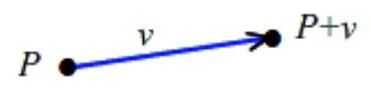
\includegraphics[max width=5cm]{2023_03_01_7659aec5e35f9a9b2d3cg-22}
\end{center}

se denomina \underline{traslación por el vector v}, y es una afinidad.

\item Si $\alpha:\mathbb{A}\longleftarrow\mathbb{A}$ es una aplicación afín con $\vec{\alpha}=Id_{V}$, entonces es una traslación.

\item El conjunto

$$
T(\mathbb{A})=\left\{t_{v}: \mathbb{A} \rightarrow \mathbb{A} \mid v \in V\right\}
$$

es un grupo abeliano con la operación composición. En particular:
\begin{itemize}
\item $t_{0} = Id_{\mathbb{A}}$
\item $t_{v}\circ t_{w} = t_{v+w}$
\item $t_{-v} = t_{v}^{-1}$
\end{itemize}

\end{enumerate}
\demostracion
\begin{enumerate}[label=(\arabic*)]
\item Si $O$ es un punto de $\mathbb{A}$, entonces

$$
\overrightarrow{t_{v}}(w):=\overrightarrow{t_{v}(O), t_{v}(O+w)}=\overrightarrow{O+v, O+w+v}=w, \quad w \in V
$$

Así, $t_{v}$ es una aplicación afín cuya aplicación lineal asociada es id $V$; además, $t_{v}$ es una afinidad, puesto que $\left(t_{v}\right)^{-1}=t_{-v}$ es una aplicación afín.

\item Para cada $P,Q\in\mathbb{A}$ sabemos que
\begin{gather*}
	\overrightarrow{\alpha(P),\alpha(Q)}=\vec{\alpha}(\overrightarrow{PQ}) = \overrightarrow{PQ}
\end{gather*}
Relación del paralelogramo
\begin{gather*}
	\overrightarrow{P,\alpha(P)} = \overrightarrow{Q,\alpha(Q)} = v
\end{gather*}
y v no depende del punto escogido, solo de $\alpha$
\begin{gather*}
	\alpha(P) = P+\overrightarrow{P,\alpha(P)} = P + v - t_{v}(P),\forall P\in\mathbb{A}
\end{gather*}

\item Se sigue de las siguientes igualdades: $t_{v+v^{\prime}}=t_{v^{\prime}} \circ t_{v}, \quad t_{0}=\operatorname{id}_{\mathbb{A}} \mathrm{y} t_{-v}=\left(t_{v}\right)^{-1}$. Habría que demostrarlas

El grupo $(T(\mathbb{A}), \circ)$ se llama grupo de traslaciones de $\mathbb{A}$ y se denota por $T(\mathbb{A})$.

\end{enumerate}


\subsubsection{Lema - Relación entre translaciones y la identidad}
Sea $\mathbb{A}$ un espacio afín sobre $V$ y $\alpha: \mathbb{A} \rightarrow \mathbb{A}$ una aplicación afín. Si $\vec{\alpha}=\operatorname{Id}_{V}$, entonces $\alpha$ es una traslación.

\demostracion

Para cada $P, Q \in \mathbb{A}$,
$$
\overrightarrow{\alpha(P), \alpha(Q)}=\overrightarrow{P Q}
$$
y por la relación del paralelogramo,
$$
\overrightarrow{P, \alpha(P)}=\overrightarrow{Q, \alpha(Q)}
$$
Pongamos $v=\overrightarrow{P, \alpha(P)}$,
$$
\alpha(P)=P+\overrightarrow{P, \alpha(P)}=P+v=t_{v}(P), \quad P \in \mathbb{A} .
$$

\subsubsection{Teorema - Isomorfismo entre los grupos $G(\mathbb{A}) / T(\mathbb{A})$ y $G L(V)$}
\noindent Los grupos $G(\mathbb{A}) / T(\mathbb{A})$ y $G L(V)$ son isomorfos.

\demostracion

\noindent Tomamos
$$
\begin{aligned}
\phi: G(\mathbb{A}) & \longrightarrow G L(V) \\
\alpha & \longmapsto \vec{\alpha}
\end{aligned}
$$
\noindent $\phi$ es un homomorfismo de grupos ya que
$$
\begin{aligned}
	\phi(\beta\circ\alpha)=\overrightarrow{\beta\circ\alpha}=\vec{\beta}\circ\vec{\alpha}=\phi(\beta)\circ\phi(\alpha)
\end{aligned}
$$

Es sobreyectiva ya que dado $f\in GL(V)$ y $A\in\mathbb{A}$, entonces $\alpha(P) = A + f(\overrightarrow{AP})$ es una afinidad con $\vec{\alpha}=f$

Veamos que $Ker(\phi)=T(\mathbb{A})$. Si $\alpha\in Ker(\phi) \longleftrightarrow \phi{\alpha} = Id_{V} \longleftrightarrow \alpha\in T(\mathbb{A})$ luego G es sobreyectiva de grupos y $G/Ker(f)$ y $H$ son isomorfos.

\ejemplos
\begin{enumerate}
\item Si $L=P+U$ es una variedad lineal de $\mathbb{A}$, entonces la aplicación inclusión $i_{L}: L \rightarrow \mathbb{A}$ es una aplicación afín; su aplicación lineal asociada es la aplicación inclusión $i_{U}: U \rightarrow V$.

\item Sea $\mathbb{A}$ un espacio afín sobre el espacio vectorial $V, \mathcal{R}=\left\{P_{1}, \ldots, P_{n} ; Q\right\}$ una referencia afín de $\mathbb{A}$ y $B_{\mathbb{R}}=\left(v_{1}, \ldots, v_{n}\right)$. La aplicación

$$
\begin{aligned}
\alpha_{\mathcal{R}}: \mathbb{A} & \longrightarrow K^{n} \\
P & \longmapsto\left(x_{1}, \ldots, x_{n}\right),
\end{aligned}
$$

donde $\left(x_{1}, \ldots, x_{n}\right)$ son las coordenadas de $P$ en $\mathcal{R}$, es una afinidad cuya aplicación lineal asociada es la aplicación

$$
\begin{aligned}
\overrightarrow{\alpha_{\mathcal{R}}}: V & \longrightarrow K^{n} \\
\sum_{i=1}^{n} z_{i} v_{i} & \longmapsto\left(z_{1}, \ldots, z_{n}\right) .
\end{aligned}
$$

En particular, si $\mathbb{A}$ es el plano (espacio) afín ordinario y $\mathcal{C}$ es la referencia canónica, la afinidad $\alpha_{\mathcal{C}}$ permite identificar el plano (espacio) ordinario con $\mathbb{R}^{2}\left(\mathbb{R}^{3}\right)$.

\item Sea $\mathbb{A}$ un espacio afín sobre el espacio vectorial $V, C$ un punto de $\mathbb{A}$ y $\lambda \in K, \lambda \neq 0$. Se llama homotecia de centro $C$ y razón $\lambda$ a la aplicación

$$
\begin{aligned}
H_{C}^{\lambda}: \mathbb{A} & \longrightarrow \mathbb{A} \\
P & \longmapsto C+\lambda \overrightarrow{C P} .
\end{aligned}
$$

\begin{center}
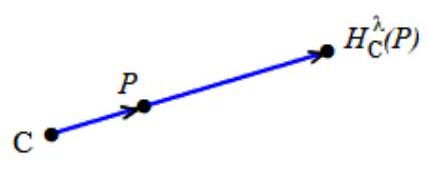
\includegraphics[max width=5cm]{2023_03_01_7659aec5e35f9a9b2d3cg-25}
\end{center}

La aplicación $\lambda \operatorname{id}_{V}: V \rightarrow V,\left(\lambda \operatorname{id}_{V}\right)(v)=\lambda v$ para todo $v \in V$, es un isomorfismo de espacios vectoriales y $H_{C}^{\lambda}(P)=C+\left(\lambda \operatorname{id}_{V}\right)(\overrightarrow{C P})$. Por las proposiciones $1.3 .5$ (1) y $1.3 .9(1), H_{C}^{\lambda}$ es una afinidad.

\item Sean $V$ y $V^{\prime}$ espacios vectoriales sobre $K$ y $f: V \rightarrow V^{\prime}$ una aplicación lineal. La aplicación $f$ considerada como aplicación entre los espacios afines de $V$ y $V^{\prime}$ es una aplicación afín. En efecto,

$$
\vec{f}(v)=\overrightarrow{f(0), f(0+v)}=f(v)-f(0)=f(v), \quad v \in V
$$

donde 0 es el vector cero de $V$.

\item Si $V$ y $V^{\prime}$ son espacios vectoriales, $v^{\prime} \in V^{\prime}$ y $f: V \rightarrow V^{\prime}$ es una aplicación lineal, entonces $t_{v^{\prime}} \circ f$ es una aplicación afín entre los espacios afines de $V$ y $V^{\prime}$, respectivamente, por ser composición de aplicaciones afines. Recíprocamente, si $\alpha: V \rightarrow V^{\prime}$ es una aplicación afín, entonces existe un vector $v^{\prime} \in V^{\prime}$ tal que $\alpha=t_{v^{\prime}} \circ \vec{\alpha}$. En efecto, por la proposición 1.3.5 (2),

$$
\alpha(P)=\alpha(0)+\vec{\alpha}(\overrightarrow{0 P})=\left(t_{\alpha(0)} \circ \vec{\alpha}\right)(P), \quad P \in V .
$$

Basta tomar $v^{\prime}=\alpha(0)$.

\end{enumerate}

\subsubsection{Proposición - Afinidades, puntos afínmente independientes y variedades lineales}
\begin{enumerate}[label=(\arabic*)]
	\item Sean $\mathbb{A}$ y $\mathbb{A}^{\prime}$ espacios afines sobre los espacios vectoriales $V$ y $V^{\prime}$, respectivamente, $\dim  \mathbb{A}=$ $\dim  \mathbb{A}^{\prime}=n$. Sea $\alpha: \mathbb{A} \rightarrow \mathbb{A}^{\prime}$ una aplicación afín y $P_{1}, \ldots, P_{n+1}$ puntos de $\mathbb{A}$ afínmente independientes. Entonces $\alpha$ es una afinidad si, y solo si, $\alpha\left(P_{1}\right), \ldots, \alpha\left(P_{n+1}\right)$ son puntos afínmente independientes.
	
	\item Sea $\alpha: \mathbb{A} \rightarrow \mathbb{A}^{\prime}$ una aplicación afín. Se tiene:
	\begin{enumerate}[label=(\alph*)]
		\item Si $L$ es una variedad lineal de $\mathbb{A}$, entonces $\alpha(L)\subset\mathbb{A}$ es una variedad lineal de $\mathbb{A}^{\prime}$.
		
		\item Si $\alpha$ es una afinidad y $L$ es una variedad lineal de $\mathbb{A}$, entonces $\dim  \alpha(L)=\dim  L$.
		
		\item $\operatorname{Si}\left\{L_{i}\right\}_{i \in I}$ es un conjunto de variedades lineales de $\mathbb{A}$, entonces
		
		$$
		\alpha\left(\circ_{i \in I} L_{i}\right)=\circ_{i \in I} \alpha\left(L_{i}\right)
		$$
		
		\noindent y si $\alpha$ es una afinidad,
		
		$$
		\alpha\left(\bigcap_{i \in I} L_{i}\right)=\bigcap_{i \in I} \alpha\left(L_{i}\right)
		$$
		
		\item Si $\alpha$ es una afinidad y $L_{1}$ y $L_{2}$ son variedades lineales de $\mathbb{A}$, entonces
		
		$$
		L_{1}\left\|L_{2} \Longleftrightarrow \alpha\left(L_{1}\right)\right\| \alpha\left(L_{2}\right)
		$$
	\end{enumerate}
\end{enumerate}

\demostracion 
\begin{enumerate}[label=(\arabic*)]
	
	\item Sean $P_{1}, \ldots, P_{n+1}$ puntos de $\mathbb{A}$ afínmente independientes. Dado que $\alpha$ es una afinidad si, y solo si, $\vec{\alpha}$ es un isomorfismo de espacios vectoriales, y que $\vec{\alpha}$ es un isomorfismo si, y solo si, los vectores
	
	$$
	\vec{\alpha}\left(\overrightarrow{P_{1} P_{2}}\right)=\overrightarrow{\alpha\left(P_{1}\right), \alpha\left(P_{2}\right)}, \ldots, \vec{\alpha}\left(\overrightarrow{P_{1} P_{n+1}}\right)=\overrightarrow{\alpha\left(P_{1}\right), \alpha\left(P_{n+1}\right)}
	$$
	
	son linealmente independientes, $\alpha$ es una afinidad si, y solo si, los puntos $\alpha\left(P_{1}\right), \ldots, \alpha\left(P_{n+1}\right)$ son afínmente independientes.
	
	\item 
	\begin{enumerate}[label=(\alph*)]
		\item Si $L=A+U$, entonces $\alpha(L)=\alpha(A)+\vec{\alpha}(U)$.
		
		\item Si $\alpha$ es una afinidad, $\dim  L=\dim _{K} U=\dim _{K} \vec{\alpha}(U)=\dim  \alpha(L)$.
		
		\item Dado que
		
		$$
		\circ_{i \in I} L_{i}=A+\left\langle\overrightarrow{A P} \mid P \in \bigcup_{i \in I} L_{i}\right\rangle, \quad A \in \bigcup_{i \in I} L_{i}
		$$
		
		se tiene
		
		\begin{gather*}
			\alpha\left(\circ_{i \in I} L_{i}\right)=\alpha(A)+\left\langle\vec{\alpha}(\overrightarrow{A P}) \mid P \in \bigcup_{i \in I} L_{i}\right\rangle=\\
			\alpha(A)+\left\langle\overrightarrow{\alpha(A), \alpha(P)} \mid \alpha(P) \in \bigcup_{i \in I} \alpha\left(L_{i}\right)\right\rangle=\circ_{i \in I} \alpha\left(L_{i}\right) .
		\end{gather*}
		
		Si $\alpha$ es una afinidad, entonces $\alpha\left(\bigcap_{i \in I} L_{i}\right)=\bigcap_{i \in I} \alpha\left(L_{i}\right)$, puesto que $\alpha$ es inyectiva.
		
		\item Sean $L_{1}=A+U_{1}, L_{2}=B+U_{2}$ y $\alpha$ una afinidad. Entonces
		
		\begin{gather*}
			L_{1} \| L_{2} \Longleftrightarrow U_{1} \subset U_{2} \text { o } U_{2} \subset U_{1} \Longleftrightarrow \\
			\Longleftrightarrow \vec{\alpha}\left(U_{1}\right) \subset \vec{\alpha}\left(U_{2}\right) \text { o } \vec{\alpha}\left(U_{2}\right) \subset \vec{\alpha}\left(U_{1}\right) \Longleftrightarrow \alpha\left(L_{1}\right) \| \alpha\left(L_{2}\right) .
		\end{gather*}
		
		El conjunto
		
		$$
		G L(V)=\{f: V \rightarrow V \mid f \text { isomorfismo de espacios vectoriales }\}
		$$
		
		es un grupo con la operación composición. El grupo $(G L(V), \circ)$ se llama grupo lineal general de $V$ y se denota por $G L(V)$.
		
	\end{enumerate}
\end{enumerate}

\subsubsection{Teorema - Clasificación de los espacios afines}
\begin{enumerate}[label=(\arabic*)]
	
	\item Todo espacio afín $(\mathbb{A}, V, \rightarrow)$ es isomorfo al espacio afín de $V$ $(V,V,\rightarrow)$.
	
	\item Dos espacios afines de igual dimensión finita son isomorfos.
	
	\item El espacio afín $\mathbb{K}^{n}$ es, salvo isomorfismos, el único espacio afín de dimensión n.
	
\end{enumerate}
\demostracion
\begin{enumerate}[label=(\arabic*)]
	
	\item Como $\mathbb{A}\ne\varnothing$, fijemos un punto $A$ de $\mathbb{A}$. La aplicación $\alpha_{A}: \mathbb{A} \rightarrow V$ dada por $\alpha_{A}(P)=\overrightarrow{A P}$ es una afinidad, En efecto,
	
	$$
	\overrightarrow{\alpha_{A}}(v)=\overrightarrow{\alpha_{A}(P), \alpha_{A}(P+v)}=\alpha_{A}(P+v)-\alpha_{A}(P)=\overrightarrow{A, P+v}-\overrightarrow{A P}=\overrightarrow{P, P+v}=v
	$$
	
	Así, $\overrightarrow{\alpha_{A}}=\operatorname{id}_{V}$
	
	\item Sean $\mathbb{A}$ y $\mathbb{A}^{\prime}$ espacios afines de la misma dimensión sobre los espacios vectoriales $V$ y $V^{\prime}$, respectivamente. Por (1), existen afinidades $\alpha: \mathbb{A} \rightarrow V$ y $\beta: \mathbb{A}^{\prime} \rightarrow V^{\prime}$. Puesto que $V$ y $V'$ tienen la misma dimensión, existe un isomorfismo de espacios vectoriales $f: V^{\prime} \rightarrow V$, y por tanto la aplicación $\beta^{-1} \circ f \circ \alpha: \mathbb{A} \rightarrow \mathbb{A}^{\prime}$ es una afinidad por composición.
	
	\item $dim_{K}V=n\Longrightarrow \exists f:V \longrightarrow K^{n}$ isomorfismo de espacios (y por tanto afinidad). Por tanto, $f \circ \alpha_{A}: \mathbb{A} \longrightarrow K^{n}$ es afinidad por composición.
	
\end{enumerate}

\subsubsection{Proposición - Isomorfismo entre espacios vectoriales y afines}
\noindent Si $\mathbb{A}$ es espacio afín sobre $V$, el grupo afín de $\mathbb{A}$ es isomorfo al grupo lineal de $V$.

\demostracion

\noindent Dado $\varphi : \mathbb{A} \longrightarrow V$ afinidad, es un isomorfismo la aplicación
$$6
\psi : G(\mathbb{A}) \longrightarrow G(V) \Longrightarrow \alpha \longmapsto \psi \circ \alpha \circ \psi^{-1}
$$

\subsection{Determinación de una aplicación afín}

\subsubsection{Teorema - Una aplicación afín está determinada unívocamente por la imagen de una referencia} Sean $\mathbb{A}$ y $\mathbb{A}^{\prime}$ espacios afines sobre los espacios vectoriales $V$ y $V^{\prime}$, respectivamente. Sea $\mathcal{R}=\left\{P_{1}, \ldots, P_{n} ; Q\right\}$ una referencia afín de $\mathbb{A}$ y $P_{1}^{\prime}, \ldots, P_{n+1}^{\prime}$ puntos de $\mathbb{A}^{\prime}$. Existe una única aplicación afín $\alpha: \mathbb{A} \rightarrow \mathbb{A}^{\prime}$ tal que $\alpha\left(P_{i}\right)=P_{i}^{\prime}, i=1, \ldots, n$, y $\alpha(Q)=P_{n+1}^{\prime}$. En particular, si $\dim  \mathbb{A}^{\prime}=n \mathrm{y}$ $P_{1}^{\prime}, \ldots, P_{n}^{\prime}, P_{n+1}^{\prime}$ son puntos afínmente independientes, entonces $\alpha$ es una afinidad.\\

\demostracion

\noindent Consideremos la aplicación lineal dada por
$$
\begin{aligned}
f: V & \longrightarrow V^{\prime} \\
\overrightarrow{Q P}_{i} & \longmapsto \vec{P}_{n+1}^{\prime} P_{i}^{\prime},
\end{aligned}
$$
\noindent y la aplicación afín
$$
\begin{aligned}
\alpha: \mathbb{A} & \longrightarrow \mathbb{A}^{\prime} \\
P & \longmapsto P_{n+1}^{\prime}+f(\overrightarrow{Q P}) .
\end{aligned}
$$
\noindent Se tiene
$$
\alpha\left(P_{i}\right)=P_{i}^{\prime}, \quad \alpha(Q)=P_{n+1}^{\prime}, \quad i=1, \ldots, n .
$$

\noindent Sea $\beta$ otra aplicación afín tal que $\beta\left(P_{i}\right)=P_{i}^{\prime}, i=1, \ldots, n$, y $\beta(Q)=P_{n+1}^{\prime}$. Entonces

$$
\overrightarrow{P_{n+1}^{\prime} P_{i}^{\prime}}=\overrightarrow{\beta(Q), \beta\left(P_{i}\right)}=\vec{\beta}\left(\overrightarrow{Q P}_{i}\right), \quad i=1, \ldots, n
$$

Por tanto, $\vec{\beta}=f$ y por la proposición 1.3.5 (3), $\beta=\alpha$. Por la proposición 1.3.9 (2), Si dim $\mathbb{A}=n$ y $P_{1}^{\prime}, \ldots, P_{n}^{\prime}, P_{n+1}^{\prime}$ son afínmente independientes, por la proposición $1.3 .9$ (2) se tiene que $\alpha$ es una afinidad.

\subsubsection{Corolario - Propiedades}
\noindent Sea $\mathcal{R}=\left\{P_{1}, \ldots, P_{n} ; Q\right\}$ una referencia afín de $\mathbb{A}$. Se tiene:

\begin{enumerate}[label=(\arabic*)]

\item Si $\alpha, \beta: \mathbb{A} \rightarrow \mathbb{A}^{\prime}$ son aplicaciones afines tales que $\alpha\left(P_{i}\right)=\beta\left(P_{i}\right), i=1, \ldots, n$, y $\alpha(Q)=\beta(Q)$, entonces $\alpha=\beta$.

\item Si $\alpha: \mathbb{A} \rightarrow \mathbb{A}$ es una aplicación afín tal que $\alpha\left(P_{i}\right)=P_{i}, i=1, \ldots, n$, y $\alpha(Q)=Q$, entonces $\alpha=\operatorname{id}_{\mathbb{A}}$.

\end{enumerate}

\ejemplo

Existe una única aplicación afín $\alpha: \mathbb{R}^{3} \rightarrow \mathbb{R}^{3}$ tal que $\alpha(1,0,0)=(2,1,2), \alpha(1,1,0)=$ $(2,0,2), \alpha(0,1,-1)=(1,1,1)$ y $\alpha(0,0,0)=(1,0,2)$, puesto que los puntos $(1,0,0),(1,1,0),(0,1,-1)$ y $(0,0,0)$ son afínmente independientes. La aplicación lineal asociada a $\alpha$ es la aplicación $\vec{\alpha}: \mathbb{R}^{3} \rightarrow \mathbb{R}^{3}$ tal que
$$
\vec{\alpha}(1,0,0)=(1,1,0), \vec{\alpha}(1,1,0)=(1,0,0), \vec{\alpha}(0,1,-1)=(0,1,-1) .
$$

\noindent Se tiene que $\vec{\alpha}(x, y, z)=(x, x-y-2 z, z)$. Por tanto,
$$
\begin{aligned}
\alpha(x, y, z) & =\alpha(0,0,0)+\vec{\alpha}(x, y, z) \\
& =(1,0,2)+(x, x-y-2 z, z)=(1+x, x-y-2 z, 2+z) .
\end{aligned}
$$

Además, $\alpha$ es una afinidad, puesto que los puntos $(2,1,2),(2,0,2),(1,1,1)$ y $(1,0,2)$ son afínmente independientes.

\subsubsection{Proposición - Aplicación afín y puntos fijos}
Si $\alpha: \mathbb{A} \rightarrow \mathbb{A}$ es una aplicación afín, $L\in\mathbb{A}$ es una variedad lineal de $\mathbb{A}$ de dimensión $r$ y $\alpha$ deja fijos $r+1$ puntos afínmente independientes de $L$, entonces $\alpha$ deja fijos todos los puntos de $L$.\\

\demostracion

Sean $L=A+U$ y $P_{1}, \ldots, P_{r+1}$ puntos de $L$ afínmente independientes y tales que $\alpha\left(P_{i}\right)=P_{i}$, para $i=1, \ldots, r+1$. Se tiene que $L=P_{1} \circ \ldots \circ P_{r+1}$ y entonces, por la proposición 1.3.9 (3) (c), $\alpha(L)=\alpha\left(P_{1}\right) \circ \ldots \circ \alpha\left(P_{r+1}\right)=P_{1} \circ \ldots \circ P_{r+1}=L$. Veamos que $\alpha_{\mid L}: L \rightarrow L$ es una aplicación afín. Dado que

$$
\overrightarrow{\alpha_{\mid L}}(u)=\overrightarrow{\alpha\left(P_{1}\right), \alpha\left(P_{1}+u\right)}=\vec{\alpha}_{\mid U}(u), \quad u \in U
$$

$\alpha_{\mid L}$ es una aplicación afín con aplicación lineal asociada $\vec{\alpha}_{\mid U}$. Por el corolario $1.3 .15(2), \alpha_{\mid L}=\operatorname{id}_{L}$.

\ejemplo

Sea $\Pi$ el plano de $\mathbb{R}^{3}$ cuya ecuación en la referencia canónica es $y-2 z=2$. Vamos a calcular la afinidad $\alpha: \mathbb{R}^{3} \rightarrow \mathbb{R}^{3}$ que deja fijos los puntos del plano $\Pi$ y tal que $\alpha(1,0,0)=(0,0,0)$.

\noindent La aplicación buscada es la aplicación afín dada por
$$
\alpha(1,2,0)=(1,2,0), \quad \alpha(0,0,-1)=(0,0,-1), \quad \alpha(0,2,0)=(0,2,0), \quad \alpha(1,0,0)=(0,0,0) .
$$

\noindent Su aplicación lineal asociada es la aplicación $\vec{\alpha}: \mathbb{R}^{3} \rightarrow \mathbb{R}^{3}$ dada por
$$
\vec{\alpha}(0,2,0)=(1,2,0), \quad \vec{\alpha}(-1,0,-1)=(0,0,-1), \quad \vec{\alpha}(-1,2,0)=(0,2,0),
$$

\noindent equivalentemente, $\vec{\alpha}(x, y, z)=(x+1 / 2 y-z, y, z)$, luego
$$
\alpha(x, y, z)=\alpha(1,0,0)+\vec{\alpha}(x-1, y, z)=(-1+x+1 / 2 y-z, y, z)
$$

La afinidad $\alpha$ deja fijos los puntos de $\Pi$, puesto que deja fijos los puntos $(1,2,0),(0,0,-1)$ y $(0,2,0)$, que son tres puntos de $\Pi$ afínmente independientes.

\subsubsection{Definición (recordatorio) - Matriz asociada a una aplicación lineal} Sean $V$ y $V^{\prime}$ espacios vectoriales sobre $K, B=\left(v_{1}, \ldots, v_{n}\right)$ una base de $V$ y $B^{\prime}=\left(v_{1}^{\prime}, \ldots, v_{m}^{\prime}\right)$ una base de $V^{\prime}$. Si $f: V \rightarrow V^{\prime}$ es una aplicación lineal y
$$
f\left(v_{i}\right)=\sum_{j=1}^{m} a_{j i} v_{j}^{\prime}, \quad i=1, \ldots, n,
$$

\noindent la matriz
$$
f_{B B^{\prime}}=\left(\begin{array}{rrr}
a_{11} & \ldots & a_{1 n} \\
\vdots & \ddots & \vdots \\
a_{m 1} & \ldots & a_{m n}
\end{array}\right)=\left(a_{i j}\right)
$$

se llama matriz asociada a $f$ respecto a las bases $B$ y $B^{\prime}$. Si $V=V^{\prime}$ y $B=B^{\prime}$ denotaremos $f_{B B^{\prime}}$ por $f_{B}$.

\subsubsection{Definición - Ecuación matricial de una aplicación afín} \noindent Sean:
\begin{itemize}

\item$V$ un espacio vectorial de dimensión $n$ y $V^{\prime}$ un espacio vectorial de dimensión $m$.
\item$\mathbb{A}$ y $\mathbb{A}^{\prime}$ espacios afines sobre $V$ y $V^{\prime}$, respectivamente, y $\alpha: \mathbb{A} \rightarrow \mathbb{A}^{\prime}$ una aplicación afín.
\item$\mathcal{R}=\left\{P_{1}, \ldots, P_{n} ; Q\right\}$ una referencia de $\mathbb{A}, \mathcal{R}^{\prime}=\left\{P_{1}^{\prime}, \ldots, P_{m}^{\prime} ; Q\right\}$ una referencia de $\mathbb{A}^{\prime}$, con $B_{\mathcal{R}}=\left(v_{1}, \ldots, v_{n}\right)$ y $B_{\mathcal{R}^{\prime}}=\left(v_{1}^{\prime}, \ldots, v_{m}^{\prime}\right)$ sus bases asociadas.

\item$\left(a_{i j}\right)$ la matriz asociada a $\vec{\alpha}$ respecto a las bases $B_{\mathcal{R}}$ y $B_{\mathcal{R}^{\prime}}$. \item$\left(x_{1}, \ldots, x_{n}\right)$ las coordenadas del punto $P \in \mathbb{A}$ en $\mathcal{R}$ y $\left(x_{1}^{\prime}, \ldots, x_{m}^{\prime}\right)$ las coordenadas de $\alpha(P)$ en $\mathcal{R}^{\prime}$.

\end{itemize}

\noindent Entonces
$$
\left(\begin{array}{c}
x_{1}^{\prime} \\
\vdots \\
x_{m}^{\prime}
\end{array}\right)=\left(\begin{array}{c}
b_{1} \\
\vdots \\
b_{m}
\end{array}\right)+\left(\begin{array}{ccc}
a_{11} & \ldots & a_{1 n} \\
\vdots & \ddots & \vdots \\
a_{m 1} & \ldots & a_{m n}
\end{array}\right)\left(\begin{array}{c}
x_{1} \\
\vdots \\
x_{n}
\end{array}\right)
$$

donde $\left(b_{1}, \ldots, b_{m}\right)$ son las coordenadas de $\alpha(Q)$ en $\mathcal{R}^{\prime}$. Esta ecuación se llama ecuación matricial de la aplicación afín $\alpha$ en las referencias $\mathcal{R}$ y $\mathcal{R}^{\prime}$.\\

\demostracion
$$
\overrightarrow{Q P}=\sum_{i=1}^{n} x_{i} v_{i}, \quad \overrightarrow{Q^{\prime} \alpha(P)}=\sum_{i=1}^{m} x_{i}^{\prime} v_{i}^{\prime}, \quad \vec{\alpha}\left(v_{j}\right)=\sum_{i=1}^{m} a_{i j} v_{i}^{\prime}, j=1, \ldots, n
$$

\noindent Puesto que $\overrightarrow{Q^{\prime} \alpha(P)}=\overrightarrow{Q^{\prime} \alpha(Q)}+\overrightarrow{\alpha(Q) \alpha(P)}=\overrightarrow{Q^{\prime} \alpha(Q)}+\vec{\alpha}(\overrightarrow{Q P})$, se tiene
$$
\sum_{i=1}^{m} x_{i}^{\prime} v_{i}^{\prime}=\sum_{i=1}^{m} b_{i} v_{i}^{\prime}+\vec{\alpha}\left(\sum_{j=1}^{n} x_{j} v_{j}\right)=\sum_{i=1}^{m} b_{i} v_{i}^{\prime}+\sum_{j=1}^{n} x_{j}\left(\sum_{i=1}^{m} a_{i j} v_{i}^{\prime}\right)=\sum_{i=1}^{m}\left(b_{i}+\sum_{j=1}^{n} a_{i j} x_{j}\right) v_{i}^{\prime},
$$

\noindent de donde se sigue
$$
x_{i}^{\prime}=b_{i}+\sum_{j=1}^{n} a_{i j} x_{j}, \quad i=1, \ldots, m
$$

Como consecuencia, se obtiene la ecuación del cambio de coordenadas ya estudiado. En efecto, la ecuación del cambio de coordenadas de la referencia $\mathcal{R}$ a la referencia $\mathcal{R}^{\prime}$ es la ecuación de la afinidad $\alpha=\operatorname{id}_{\mathbb{A}}: \mathbb{A} \rightarrow \mathbb{A}$ en las referencias $\mathcal{R}$ y $\mathcal{R}^{\prime}$. Si $L$ es una variedad lineal de $\mathbb{A}, \mathcal{R}^{\prime}$ es una referencia de $L$ y $\mathcal{R}$ es una referencia de $\mathbb{A}$, la ecuación de cambio de coordenadas de los puntos de $L$ de la referencia $\mathcal{R}^{\prime}$ a $\mathcal{R}$ es la ecuación de inclusión $i_{L}: L \rightarrow \mathbb{A}$ en las referencias $\mathcal{R}^{\prime}$ y $\mathcal{R}$.

\begin{center}
\section{Espacios Vectoriales Euclídeos}
\end{center}

En este tema se introduce el concepto de producto escalar en un espacio vectorial real, que generaliza el concepto de producto escalar usual de vectores libres del plano o espacio. Trasladaremos a los espacios vectoriales euclídeos las nociones de longitud de un vector y ángulo entre dos vectores, de forma que se conserven las propiedades que tienen en el espacio vectorial de los vectores libres.

Probaremos la existencia de bases ortonormales en un espacio vectorial euclídeo de dimensión finita. Las transformaciones ortonormales de un espacio vectorial euclídeo son las aplicaciones lineales que conservan el producto escalar o, equivalentemente, la longitud de los vectores. Se estudian y clasifican las transformaciones ortogonales de un plano y de un espacio vectorial euclídeo tridimensional.

\subsection{Preliminares}

\subsubsection{Definición - Ortogonalidad entre vectores}
\noindent Sean $u,v \in V$. Se dice que son ortogonales si $u\cdot v = 0$.

\subsubsection{Definición - Producto escalar} Sea $V$ un espacio vectorial real. Se dice que una aplicación $\sigma: V \times V \rightarrow \mathbb{R}$ es un producto escalar en $V$ si verifica las siguientes condiciones:

\begin{enumerate}[label=(\arabic*)]
	
	\item $\sigma$ es una aplicación bilineal o una forma bilineal, es decir:
	\begin{enumerate}[label=(\alph*)]
		\item $\sigma\left(\lambda_{1} v_{1}+\lambda_{2} v_{2}, w\right)=\lambda_{1} \sigma\left(v_{1}, w\right)+\lambda_{2} \sigma\left(v_{2}, w\right), \quad v_{1}, v_{2}, w \in V, \lambda_{1}, \lambda_{2} \in \mathbb{R}$,
		\item $\sigma\left(v, \lambda_{1} w_{1}+\lambda_{2} w_{2}\right)=\lambda_{1} \sigma\left(v, w_{1}\right)+\lambda_{2} \sigma\left(v, w_{2}\right), \quad v, w_{1}, w_{2} \in V, \lambda_{1}, \lambda_{2} \in \mathbb{R}$,
	\end{enumerate}
	\item $\sigma$ es simétrica, es decir $\sigma(v, w)=\sigma(w, v)$, para todo $v, w \in V$,
	
	\item $\sigma$ es definida positiva:
	
	\begin{enumerate}[label=(\alph*)]
		\item $\sigma(v, v) \geq 0$, para todo $v \in V$,
		
		\item $\sigma(v, v)=0 \quad \Rightarrow \quad v=0$.
	\end{enumerate}
\end{enumerate}
Si $\sigma$ es un producto escalar, denotaremos con frecuencia $\sigma(u, v)$ por $u \cdot v$.

Un espacio vectorial euclídeo es un par $(V, \sigma)$, donde $V$ es un espacio vectorial real y $\sigma$ es un producto escalar en $V$. Lo denotaremos por $(V, \sigma)$ o simplemente por $V$.

\subsubsection{Cuestión}
Sea $v \in V$, definimos la ''norma'' o longitud de $v$, y la denotamos $\|v\| = \sqrt{v \cdot v}$. Decimos que v es unitario si $\|v\| = 1$.

\underline{Cuestión:}
¿Es esta longitud con la ''norma'' una norma ''de verdad''?

\subsubsection{Definición - Norma}
\noindent Una norma en V es una aplicación $\|\cdot\| : V \longrightarrow \mathbb{R}$ satisfaciendo:
\begin{enumerate}
	\item $\|u + v \| \le \|u\| + \|v\|$.
	\item $\|\lambda \cdot v\| = |\lambda| \cdot \|v\|, \; \forall v \in V, \lambda \in \mathbb{R}$.
	\item $\|v\| > 0, \forall v \in V - \{0\}$.
\end{enumerate}

\subsubsection{Teorema - Propiedades de una norma}
\noindent Sea $V$ un espacio vectorial euclídeo. Entonces:
\begin{enumerate}
	\item  $\|u + v \| \le \|u\| + \|v\|$. Además, $\|v\| = 0 \Longleftrightarrow v = 0$.
	\item $\|\lambda v\| = |\lambda| \cdot \|v\| \space, \; \forall v \in V, \lambda \in \mathbb{R}$.
	\item (Desigualdad de Cauchy-Schwarz) 
	$|u \cdot v| \le \|u\| \cdot \|v\|$.
	\item (Desigualdad Triangular) $\|u + v\| \le \|u\| + \|v\|$.
	\item (Teorema de Pitágoras) Si $u \cdot v = 0$, $\|u + v\|^{2} = \|u\|^{2} + \|v\|^{2}$.
\end{enumerate}
\demostracion
\begin{enumerate}
	\item No la hizo.
	\item No la hizo.
	\item Si $u = 0$ o $v = 0$, es trivial. Supongamos que no es el caso. Para cada $\lambda \in \mathbb{R}$, tenemos:
	\begin{align*}
		\|\lambda u - v\|^{2} = (\lambda u - v) (\lambda u - v) = \lambda^{2} \|u\|^{2} + \|v\|^{2} - 2 \lambda u \cdot v \Longrightarrow
	\end{align*}
	\begin{align*}
		\Longrightarrow 2 \lambda u \cdot v \le \lambda^{2} \|u\|^{2} + \|v\|^{2}, \forall \lambda \in \mathbb{R} / u, v \ne 0.
	\end{align*}
	Tomemos $\lambda = \frac{u \cdot v}{\|u\|^{2}}$
	\begin{align*}
		2 \frac{u \cdot v}{\|u\|^{2}} u \cdot v \le \left(\frac{u \cdot v}{\|u\|^{2}}\right) \|u\|^{2} + \|v\|^{2} \Longrightarrow |u \cdot v| \le \|u\| \cdot \|v\|.
	\end{align*}
	
	\underline{Cuestión:} ¿Cuándo se da la igualdad en C-S?\\
	
	\underline{Ejemplo:} Encontrar el máximo de la función
	\begin{align*}
		f: \; \$^{2} & \longrightarrow \mathbb{R} \\
		(x,y,z) & \longmapsto f(x,y,z) = x + 2y + 3z
	\end{align*}
	Tomemos los vectores $(x, y, z)$ y $|(x, y, z) \cdot (1, 2, 3)| \le \|(x, y, z)\| \cdot \|(1, 2, 3)\| = \sqrt{x^{2} + y^{2} + z^{2}}$. Lo borró T\_T.
	\item $\|u + v \|^{2} = (u + v) (u + v) = u \cdot u + v \cdot v + 2u \cdot v \le u \cdot u + v \cdot v + |2u \cdot v| = \|u\|^{2} + \|v\|^2 + 2|u \cdot v| \le \|u\|^{2} + \|v\|^{2} + 2\|u\|\,\|v\|$.
	\item $\|u + v \|^{2} = |u \cdot u + v \cdot v + 2uv| = \|u\|^{2} + \|v\|^{2}$.
	La igualdad en $(4)$: $2uv = 2\|u\|\,\|v\|$. Si tenemos la igualdad en $(4)$, entonces la tenemos en $(3)$. Si el ángulo entre $u$ y $v$ es 0, entonces $u \cdot v = \|u\|\,\|v\|$. Ahora, si
	\begin{align*}
		u,v \ne 0 \Longrightarrow -\|u\|\,\|v\| \le u \cdot v \le \|u\|\,\|v\| \Longrightarrow -1 \le \frac{u \cdot v}{\|u\|\,\|v\|} \le 1
	\end{align*}
	Ahora, sea $cos: [0,\pi] \longrightarrow [-1,1]$. Definimos $\angle(u,v)$ como el único número real tal que
	\begin{align*}
		cos(\angle(u,v)) = \frac{u \cdot v}{\|u\|\,\|v\|}
	\end{align*}
	La igualdad se da cuando $\|\lambda u - v\|^{2} \Longleftrightarrow \lambda u - v = 0 \Longleftrightarrow \exists \lambda \in \mathbb{R} \,/\, v = \lambda u \Longleftrightarrow u$ y $v$ son linealmente independientes.
	
	\underline{Cuestión:} Decidir si $\sigma : VxV \longrightarrow \mathbb{R}$ es producto escalar.\\
	\underline{Objetivo:} encontrar bases ''buenas'' de $V$.
\end{enumerate}

\subsubsection{Definición - Base ortonormal} Sea $(V,\sigma)$ euclídeo, decimos que la base $\{v_{1},...,v_{n}\}$ de $V$ es ortonormal si cada vector es ortogonal al resto: $v_{i} \cdot v_{j} = \delta_{ij}$, es decir, la matriz de Gram del producto escalar es la identidad.

\ejemplo

Base canónica de $\mathbb{R}^{n}$ con el producto escalar usual.

\subsubsection{Propiedad 1}
Sea $x = (x_1,...,x_n) \in \mathbb{R}$. Entonces:
\begin{align*}
	\|x\| = \sqrt{\sum_{}^{}x_i^2}\\
\end{align*}
Con $\sigma: \mathbb{R}^n \times \mathbb{R}^n \longrightarrow \mathbb{R}$ producto escalar usual, su matriz de Gram es la identidad:
\begin{align*}
	G = \left(
	\begin{matrix}
		1 &        & 0 \\
		& \ddots &   \\
		0 &        & 1
	\end{matrix}
	\right) = I
\end{align*}

\subsubsection{Propiedad 2.}
Sea $\{v_1,...,v_n\}$ un conjunto e vectores no nulos y ortogonales dos a dos. Entonces, son linealmente independientes.

\demostracion
\begin{align*}
	\sum_{i=1}^{n} \lambda_i v_i = 0 \Longrightarrow \lambda_i = 0, \forall i \in \{1,...,n\}\\
	v_j \left( \sum_{i=1}^{n} \lambda_i v_i \right) = \lambda_j v_j \cdot v_j \Longrightarrow \lambda_j = 0
\end{align*}

\subsubsection{Teorema - Método de ortogonalización de Gram-Schmidt}
\noindent Sea $V$ un espacio vectorial euclídeo. Si $B = \{u_1,...,u_n\}$ es una base, entonces
\begin{align*}
	&v_1 = u_1 \\
	&v_i = u_i - \sum_{j=1}^{i-1} \frac{u_i \cdot v_j}{\|v_j\|^2} v_j, i \in \{2,...,n\}
\end{align*}
forma una base ortogonal de $V$.

\demostracion

\noindent Inducción (ejercicio).

\observacion

$B$ base es una hipótesis innecesaria, se puede partir de un conjunto de vectores linealmente independientes y obtener otro conjunto linealmente independiente de la misma cardinalidad.

\subsubsection{Teorema - Existencia de bases ortonormales}
Sea $(V,\sigma)$ un espacio vectorial euclídeo de dirección finita. Entonces, existe una base ortonormal.

\demostracion

$B \longrightarrow B'$ ortogonal (Gram-Schmidt). $B'=\{v_1,...,v_n\}$, $B''=\left\{\frac{v_1}{\|v_1\|},...,\frac{v_n}{\|v_n\|}\right\}$. Se tiene que:
$$
\frac{v_i}{\|v_i\|} \cdot \frac{v_j}{\|v_j\|} =
\begin{cases}
	0 \text{ si } i \ne j \\
	\displaystyle \frac{v_j \cdot v_i}{\|v_i\| \cdot \|v_j\|} = \frac{v_i \cdot v_i}{\|v_i\|^2} = \frac{1}{1^2} = 1 \text{ si } i = j
\end{cases}
$$

\subsubsection{Corolario - Congruencia de la matriz de Gram y la identidad}
\noindent Sea $(V,\sigma)$ un espacio vectorial euclídeo de dimensión finita. Entonces, la matriz de Gram siempre es congruente a la identidad:
\begin{align*}
	& G_\sigma^B \cong \operatorname{Id} \\
	& G_\sigma^B = P^T\operatorname{Id}P
\end{align*}

\underline{Consecuencia:} Dos espacios vectoriales euclídeos son isométricos $\Longleftrightarrow$ tienen la misma dimensión.

\noindent \underline{Cuestión:} Cuándo es (V,$\sigma$) un espacio vectorial simétrico?
\begin{itemize}
	\item $\sigma$ fuese simétrica ($G_\sigma^B$ simétrica).
	\item $\sigma$ sea definida positiva ($\sigma(v,v)=v \cdot v > 0, \; \forall v \in v - \{0\}$).
\end{itemize}

\subsubsection{Recordatorio - Propiedades de los determinantes}
\begin{enumerate}[label=(\arabic*)]
	\item Al cambiar dos columnas de la matriz, cambia el signo.
	\item Multiplicar una columna por un escalar es multiplicar el determinante por el escalar.
	\item Lineal en cada componente.
	\item $\det(Id) = 1$
	\item $\det(AB) = det(A) \cdot det(B)$
\end{enumerate}
\observacion

Se puede pensar en el determinante en $\mathbb{R}^2$ como el área que forman los vectores columna de la matriz. De la misma forma, en $\mathbb{R}^3$ sería el volumen.

\subsubsection{Teorema - Criterio de Sylvester.}
Sea $(V,\sigma)$ un espacio vectorial dotado de una aplicación bilineal simétrica, $B = \{v_1,...,v_n\}$ una base de $V$, y $G_\sigma^B = (g_{ij})$ la matriz de Gram asociada. Entonces, $\sigma$ es definida positiva $\Longleftrightarrow \det(\Delta_i) > 0, \forall i \in \{1,...,n\}$, donde

\begin{align*}
	\Delta_i = \left(
	\begin{matrix}
		g_{11} & ... & g_{1i} \\
		\vdots &     & \vdots \\
		g_{i1} & ... & g_{ii}
	\end{matrix}
	\right)
\end{align*}

\demostracion

\dobleimplicacion{
Queremos expresar los menores respecto de la base. Dada $B_j = \{v_1, \ldots, v_j\}$ tenemos el subespacio $V_j = \langle B_j \rangle$ y la aplicación restringida $\sigma_j = \sigma|_{V_j}$. $(V_j, \sigma_j)$ es un espacio euclídeo, luego existe una base ortonormal (tiene asociada la identidad). Por tanto, $\exists P_j$ regular tal que $G_j = P_j^T \operatorname{Id} P_j$ con $j = 1,\ldots,n$. El determinante será $\det(\Delta_j) = \det(P_j^T) \det(\operatorname{Id}) \det(P_j) = P_j^2 > 0$. Luego $\det(\Delta_j) > 0, \; \forall j = 1,\ldots,n$.
}{
Para probar el recíproco, razonaremos por inducción sobre la dimensión de $V$. Si la dimensión de $V$ es 1 , el resultado es cierto trivialmente. Supongamos el resultado cierto para espacios vectoriales de dimensión $n-1$ y veamos que es cierto para espacios vectoriales de dimensión $n$.

Sea $V$ un espacio vectorial de dimensión $n, \sigma: V \times V \rightarrow \mathbb{R}$ una forma bilineal simétrica y $B=\{v_{1}, \ldots, v_{n}\}$ una base de $V$ tal que $\Delta_{i}>0$, para $i=1, \ldots, n$. La idea es encontrar una base $\widetilde{B}$ de $V$ tal que $v^t G_\sigma^{\widetilde{B}} v > 0, \forall v \in V - \{0\}$.

Sea $V^{\prime}=\left\langle v_{1}, \ldots, v_{n-1}\right\rangle$ y $\sigma^{\prime}=\sigma_{\left.\right|_{V^{\prime}}}$. Dado que $\Delta_{i}>0$, para $i=1, \ldots, n-1$, por hipótesis de inducción $\sigma^{\prime}$ es definida positiva, luego $\left(V^{\prime}, \sigma^{\prime}\right)$ es un espacio vectorial euclídeo. Sea $B^{\prime}=\left(w_{1}, \ldots, w_{n-1}\right)$ una base ortonormal de $V^{\prime}$. Pongamos $B^{\prime \prime}=\left(w_{1}, \ldots, w_{n-1}, v_{n}\right)$. Se tiene

$$
G_{\sigma}^{B^{\prime \prime}}=\left(\begin{array}{ccccc}
	1 & 0 & \ldots & 0 & c_{1} \\
	0 & 1 & \ldots & 0 & c_{2} \\
	\vdots & \vdots & & \vdots & \vdots \\
	0 & 0 & \ldots & 1 & c_{n-1} \\
	c_{1} & c_{2} & \ldots & c_{n-1} & c_{n}
\end{array}\right)
$$

Sabemos que existe una matriz regular $Q$ tal que $G_{\sigma}^{B^{\prime \prime}}=\mathcal{Q}^{t} G_{\sigma}^{B} \mathcal{Q}$. Consideremos la matriz

$$
\mathcal{P}=\left(\begin{array}{ccccc}
	1 & 0 & \ldots & 0 & -c_{1} \\
	0 & 1 & \ldots & 0 & -c_{2} \\
	\vdots & \vdots & & \vdots & \vdots \\
	0 & 0 & \ldots & 1 & -c_{n-1} \\
	0 & 0 & \ldots & 0 & 1
\end{array}\right)
$$

Se tiene

$$
\mathcal{P}^{t} G_{\sigma}^{B^{\prime \prime}} \mathcal{P}=\operatorname{diag}\left(1,\ldots,1,d\right), \quad d=c_{n}-c_{1}^{2}-\ldots-c_{n-1}^{2} .
$$

Sea $\mathcal{T}=\mathcal{Q} \mathcal{P}$. Entonces $\mathcal{T}^{t} G_{\sigma}^{B} \mathcal{T}=\operatorname{diag}\left(1,\ldots,1,d\right)$, luego

$$
d=\det(\mathcal{T})^{2} \det\left(G_{\sigma}^{B}\right)>0
$$

Sea $\widetilde{B}$ la base tal que $\mathcal{T}=i d_{\tilde{B} B}$. Se tiene que $G_{\sigma}^{\widetilde{B}}=\operatorname{diag}\left(1,\ldots,1,d\right)$. La forma bilineal $\sigma$ es definida positiva, puesto que si $v \in V-\{0\}$ tiene coordenadas $\left(x_{1}, \ldots, x_{n}\right)$ en la base $\tilde{B}$, entonces

$$
v \cdot v=x_{1}^{2}+\ldots+x_{n-1}^{2}+d x_{n}^{2}>0
$$
}
\ejemplo

La forma bilineal $\sigma: \mathbb{R}^{3} \times \mathbb{R}^{3} \rightarrow \mathbb{R}$ dada por
$$
\sigma\left(\left(x_{1}, x_{2}, x_{3}\right),\left(y_{1}, y_{2}, y_{3}\right)\right) = 2 x_{1} y_{1}-x_{1} y_{2}-x_{2} y_{1}+x_{2} y_{2}-x_{2} y_{3}-x_{3} y_{2}+3 x_{3} y_{3}
$$
tiene como matriz de Gram en la base canónica $C=\left(e_{1}=(1,0,0), e_{2}=(0,1,0), e_{3}=(0,0,1)\right)$

$$
G_{\sigma}^{C}=\left(\begin{array}{rrr}
	2 & -1 & 0 \\
	-1 & 1 & -1 \\
	0 & -1 & 3
\end{array}\right)
$$
La forma bilineal $\sigma$ es simétrica, puesto que $\left(G_{\sigma}^{C}\right)^{t}=G_{\sigma}^{C}$. Además,

$$
\det(2)=2>0, \quad\left|\begin{array}{rr}
	2 & -1 \\
	-1 & 1
\end{array}\right|=1>0, \quad \det\left(G_{\sigma}^{C}\right)=1>0
$$

luego $\sigma$ es definida positiva, por el criterio de Sylvester. Así, $\sigma$ es un producto escalar en $\mathbb{R}^{3}$.

Vamos a calcular una base ortogonal $B^{\prime}=\left(w_{1}, w_{2}, w_{3}\right)$ de $\left(\mathbb{R}^{3}, \sigma\right)$ aplicando el método de ortogonalización de Gram-Schmidt a la base canónica de $\mathbb{R}^{3}$ (tomando $\sigma$ como un producto escalar):
$$
\begin{aligned}
	& w_{1}=e_{1}=(1,0,0) \\
	& w_{2}=e_{2}-\frac{e_{2} w_{1}}{\|w_{1}\|^2} w_{1}=(0,1,0)-(-1 / 2)(1,0,0)=(1 / 2,1,0) \\
	& w_{3}=e_{3}-\frac{e_{3} w_{1}}{\|w_{1}\|^2} w_{1}-\frac{e_{3} w_{2}}{\|w_{2}\|^2} w_{2}=(0,0,1)-(-2)(1 / 2,1,0)=(1,2,1) .
\end{aligned}
$$
Obsérvese que
$$
\sigma\left(e_{3}, w_{2}\right)=\left(\begin{array}{lll}
	0 & 0 & 1
\end{array}\right)\left(\begin{array}{rrr}
	2 & -1 & 0 \\
	-1 & 1 & -1 \\
	0 & -1 & 3
\end{array}\right)\left(\begin{array}{r}
	1 / 2 \\
	1 \\
	0
\end{array}\right)=-1
$$
y de forma análoga se obtiene que $\sigma\left(w_{2}, w_{2}\right)=1 / 2$. La base $B^{\prime}$ no es ortonormal, puesto que los vectores $w_{1}$ y $w_{2}$ no son unitarios
$$
\left\|w_{1}\right\|=\sqrt{\sigma\left(w_{1}, w_{1}\right)}=\sqrt{2}, \quad\left\|w_{2}\right\|=\sqrt{\sigma\left(w_{2}, w_{2}\right)}=\sqrt{2} / 2, \quad\left\|w_{3}\right\|=\sqrt{\sigma\left(w_{3}, w_{3}\right)}=1
$$
A partir de $B^{\prime}$ se obtiene la siguiente base ortonormal de $\left(\mathbb{R}^{3}, \sigma\right)$ :
$$
B=\left(\frac{w_{1}}{\left\|w_{1}\right\|}, \frac{w_{2}}{\left\|w_{2}\right\|}, \frac{w_{3}}{\left\|w_{3}\right\|}\right)=((\sqrt{2} / 2,0,0),(\sqrt{2} / 2, \sqrt{2}, 0),(1,2,1)) .
$$

\subsection{Espacios vectoriales euclídeos}

\subsubsection{Definición - Ortogonalidad entre subespacios}
Sean $(V, \sigma)$ un espacio euclídeo y $U$ y $W$ subespacios de $V$. Se dice que $U$ es ortogonal a $W$ si $u \cdot w=0$ para todo $u \in U$ y para todo $w \in W$.

\subsubsection{Definición - Suma ortogonal de subespacios}
Sea $V$ un espacio vectorial euclídeo y sean $U$ y $W$ subespacios de $V$. Se dice que la suma $U+W$ es una suma ortogonal y se denota por $U \perp W$, si verifica que $U \cap W=\{0\}$ y $U$ es ortogonal a $W$ (es decir, $u \cdot w = 0, \; \forall u \in U, w\in W$).

\subsubsection{Definición - Subespacio ortogonal a uno dado}
\noindent Sea $V$ un espacio vectorial euclídeo y $U$ un subespacio de $V$. El subespacio
$$
U^{\perp}=\{v \in V \mid u \cdot v=0, \forall u \in U\}
$$
se llama subespacio ortogonal a $U$.

\subsubsection{Proposición}
Sea $V$ un espacio vectorial euclídeo y $U$ un subespacio de $V$ de dimensión finita. Se tiene que $V=U \perp U^{\perp}$.
\demostracion

Sea $B=\{u_{1}, \ldots, u_{r}\}$ una base ortonormal de $U$ y $v \in V$. Consideremos el vector
$$
u=\left(v \cdot u_{1}\right) u_{1}+\ldots+\left(v \cdot u_{r}\right) u_{r} \in U
$$
El vector $v-u \in U^{\perp}$, puesto que, para cada $i=1, \ldots, r$
$$
(v-u) \cdot u_{i}=v \cdot u_{i}-u \cdot u_{i}=v \cdot u_{i}-v \cdot u_{i}=0, \quad i=1, \ldots, r
$$
Así, $V=U+U^{\perp}$. Además, si $v \in U \cap U^{\perp}$, entonces $v \cdot v=0$ y por ser $V$ un espacio vectorial euclídeo, se tiene que $v=0$. Por tanto $V=U \perp U^{\perp}$.

Los números reales $v \cdot u_{i}$ se llaman coeficientes de Fourier de $v$ respecto a la base ortonormal $B$ de $U$.

\observacion

Si tenemos una base ortonormal de un espacio euclídeo $V$, $B = \{v_1,\ldots,v_n\}$ y $v = (x_1,\ldots,x_n)\in V$. Entonces $x_i = v \cdot v_i$.

\subsubsection{Definición - Proyección ortogonal de un vector sobre un subespacio} Sea $V$ un espacio vectorial euclídeo y $U$ un subespacio de $V$ de dimensión finita. Si $v \in V$ se llama proyección ortogonal de $v$ sobre $U$ al vector $v_{U} \in U$ tal que $v-v_{U} \in U^{\perp}$.

\begin{center}
	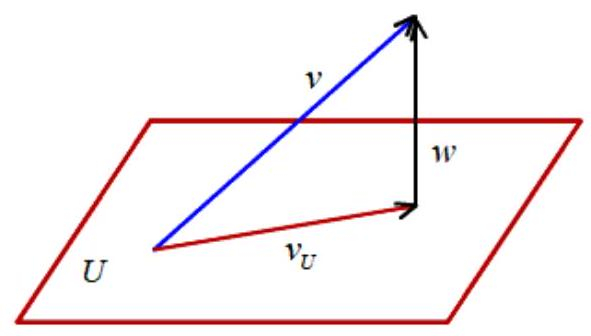
\includegraphics[max width=5cm]{2023_03_20_c2fe6c117849a1a0e8afg-048}
\end{center}
\observacion

Sea $V$ un espacio vectorial euclídeo, $U$ es un subespacio de $V$ de dimensión finita y $v$ un vector de $V$. Si $B=\left(u_{1}, \ldots, u_{r}\right)$ es una base ortonormal de $U$, entonces

$$
v_{U}=\left(v \cdot u_{1}\right) u_{1}+\ldots+\left(v \cdot u_{r}\right) u_{r} \in U
$$

Veamos un ejemplo de como calcular la proyección ortogonal de un vector sobre un plano vectorial de $\mathbb{R}^{3}$.

\ejemplo

Consideremos el plano vectorial $U$ de $\mathbb{R}^{3}$ cuya ecuación en la base canónica es $2 x+y-z=0$ y el vector $v=(-3,1,1)$. Se tiene

$$
U=\left\langle(1,0,2),(0,1,1)\rangle, \quad U^{\perp}=\langle(2,1,-1)\rangle\right.
$$
Luego $\mathbb{R}^{3}=U \perp U^{\perp}=\langle(1,0,2),(0,1,1),(2,1,-1)\rangle$. Dado que

$$
(-3,1,1)=-(1,0,2)+2(0,1,1)-(2,1,-1),
$$
la proyección ortogonal de $v$ sobre $U$ es el vector

$$
v_{U}=-(1,0,2)+2(0,1,1)=(-1,2,0) .
$$

\subsection{Producto vectorial}
\subsubsection{Definición - Orientación de una base}
Sea $V$ un espacio vectorial de dimensión finita. Decimos que dos bases $B$ y $B'$ tienen la misma orientación si $\det(\operatorname{Id}_{BB'})>0$. En caso contrario, diremos que tienen distinta orientación.

\ejemplos
\begin{enumerate}
	\item La base $\{e_1,e_2\}$ de $\mathbb{R}^2$ es de orientación positiva.
	\item La base $\{(1,0),(1,1)\}$ de $\mathbb{R}^2$ es de orientación positiva.
\end{enumerate}
\underline{Observación}\\
El orden en la base importa en este caso, ponemos paréntesis en vez de corchetes: $B=(v_1,\ldots,v_n)$.

\subsubsection{Notación - Clase de equivalencia de la orientación}
Se denota por $[B]$ a la clase de equivalencia respecto de la orientación. Diremos que la orientación positiva es la de la base canónica (en el caso de $\mathbb{R}^n$).

\subsubsection{Definición - Producto vectorial}
Sea $B = (v_1,v_2,v_3)$ una base ortonormal de un espacio V de dimensión $3$ y positivamente orientada. Sean $u = (x_1,x_2,x_3)$ y $v = (y_1,y_2,y_3)$. Se define el producto vectorial como
$$
u \wedge v = \left(\left|
\begin{matrix}
	x_2 & x_3 \\
	y_2 & y_3
\end{matrix}
\right| , \left|
\begin{matrix}
	x_3 & x_1 \\
	y_3 & y_1
\end{matrix}
\right| , \left|
\begin{matrix}
	x_1 & x_2 \\
	y_1 & y_2
\end{matrix}
\right|
\right)
$$

\subsubsection{Proposición - Propiedades del producto vectorial}
\begin{enumerate}
	\item Los vectores $u$ y $v$ no nulos son linealmente dependientes $\Longleftrightarrow u \wedge v = 0$.
	\item $u \wedge v$ es ortogonal a $u$ y a $v$.
	\item Si $u$ y $v$ son linealmente independientes, entonces $(u,v,u \wedge v)$ son una base de $V$ positivamente orientado.
	\item $\|u \wedge v \| = \|u\| \cdot \|v\| \cdot \operatorname{sen} \angle (u,v) = \|u\| \cdot \|v\| \cdot \operatorname{sen} \angle (v,u)$.
	\item La aplicación
	\begin{align*}
		\wedge : V \times V & \longrightarrow V \\
		(u,v) & \longmapsto u \wedge v
	\end{align*}
	es bilineal y antisimétrica.
\end{enumerate}
\demostracion\\
\begin{enumerate}
	\item $u$ y $v$ son linealmente dependientes $\Longleftrightarrow \operatorname{rango} \left(
	\begin{matrix}
		x_1 & x_2 & x_3 \\
		y_1 & y_2 & y_3
	\end{matrix}
	\right) = 1 \Longleftrightarrow \left|
	\begin{matrix}
		x_2 & x_3 \\
		y_2 & y_3
	\end{matrix}
	\right| = 0, \left|
	\begin{matrix}
		x_3 & x_1 \\
		y_3 & y_1
	\end{matrix}
	\right| = 0, \left|
	\begin{matrix}
		x_1 & x_2 \\
		y_1 & y_2
	\end{matrix}
	\right| = 0 \Longleftrightarrow u \wedge v = 0$
	\item $u \cdot (u \wedge v) = x_1 \left|
	\begin{matrix}
		x_2 & x_3 \\
		y_2 & y_3
	\end{matrix}
	\right| + x_2 \left|
	\begin{matrix}
		x_3 & x_1 \\
		y_3 & y_1
	\end{matrix}
	\right| + x_3 \left|
	\begin{matrix}
		x_1 & x_2 \\
		y_1 & y_2
	\end{matrix}
	\right| = \left| \begin{matrix}
		x_1 & x_2 & x_3 \\
		x_1 & x_2 & x_3 \\
		y_1 & y_2 & y_3
	\end{matrix}
	\right| = 0$
	\item Como $\{u,v,u \wedge v\}$ son linealmente independientes, forman una base. Es cierto que...
	$$
	\text{¿} \lambda u + \beta v + \gamma (u \wedge v) = 0 \Longrightarrow \lambda = \beta = \gamma = 0 \text{?}
	$$
	Utilizando la propiedad (1):
	$$
	(u \wedge v) = (\lambda u + \beta v + \gamma (u \wedge v)) = 0 \Longrightarrow \gamma (u \wedge v)(u \wedge v) = 0 \Longrightarrow \lambda = 0
	$$
	Ahora tenemos que ver que está positivamente orientada.
	$$
	\operatorname{Id}_{B'B} =
	\begin{pmatrix}
		x_1 & y_1 & \begin{vmatrix}
			x_2 & x_3 \\
			y_2 & y_3
		\end{vmatrix} \\
		x_2 & y_2 & \begin{vmatrix}
			x_3 & x_1 \\
			y_3 & y_1
		\end{vmatrix}\\
		x_3 & y_3 & \begin{vmatrix}
			x_1 & x_2 \\
			y_1 & y_2
		\end{vmatrix}
	\end{pmatrix}
	$$
	$\det(\operatorname{Id}_{B'B})$
	\item Se tiene:
	\begin{align*}
		\|u \wedge v\|^2 & = \|u\|^2 \cdot \|v\|^2 \operatorname{sen} 	\angle (u,v) \\
		& = \|u\|^2 \cdot \|v\|^2 - \|u\|^2 \cdot \|v\|^2 	\operatorname{cos} \angle (u,v) \\
		& = (x^2_1 + x^2_2 + x^2_3)(y^2_1 + y^2_2 + y^2_3) - 
		(x_1 y_1 + x_2 y_2 + x_3 y_3)
	\end{align*}
	\item Inmediato por definición de los determinantes.
\end{enumerate}

\subsubsection{Proposicion}
Si $u$ y $v$ son vectores linealmente independientes, entonces $u \wedge v$ está determinado por (2), (3) y (4). Así, $u \wedge v$ no depende de la base ortonormal de orientación positiva escogida.

\demostracion

Sea $w \in V$ satisfaciendo (2), (3) y (4).
\begin{align*}
	& \text{(2)} \Longrightarrow  
	\begin{cases}
		u \cdot w = 0 \\
		v \cdot w = 0
	\end{cases}
	\Longrightarrow
	\begin{cases}
		w \in <u,v>^\bot \\
		<w> = <u,v>^\bot
	\end{cases}\\
	& \operatorname{dim}(V) = 3 \Longrightarrow <w> = <u \cdot w> \Longrightarrow \exists \lambda \in \mathbb{R} : w = \lambda \cdot (u \wedge v)
	\Longrightarrow \\
	& \|w\| = \|u\| \cdot \|v\| \operatorname{sen}(u,v) \Longrightarrow |\lambda| = 1 \Longrightarrow \begin{cases}
		\lambda_1 = 1 \\
		\lambda_2 = -1
	\end{cases}
\end{align*}

\subsection{Producto mixto}
\noindent Sea $B$ una base de $V$, ortonormal y de orientación positiva. Sea $u$, $v$ y w vectores de $V$.
$$
(uvw) = u(v \wedge w)
$$

\subsubsection{Propiedades del producto mixto}
\begin{enumerate}
	\item Sean $u = (x_1, x_2, x_3), v = (y_1, y_2, y_3), w = (z_1, z_2, z_3)$. Entonces:\\
	$$
	(uvw) =
	\begin{vmatrix}
		x_1 & x_2 & x_3 \\
		y_1 & y_2 & y_3 \\
		z_1 & z_2 & z_3
	\end{vmatrix}
	$$
	\item $(uvw) = (vwu) = (wuv)$
\end{enumerate}

\subsection{Grupos}

\subsubsection{Definición - Grupo}
Un grupo es un par $(\mathcal{G}, *)$, donde $\mathcal{G}$ es un conjunto y $*$ es una operación binaria satisfaciendo:
\begin{enumerate}
	\item Es asociativa
	\item Existe elemento neutro
	\item $\forall g \in \mathcal{G}, \; \exists g^{-1}$ (inversa)
\end{enumerate}

\subsubsection{Definición - Actuación de un grupo sobre un conjunto}
Sean $\mathcal{G}$ un grupo y $A$ un conjunto. Decimos que $\mathcal{G}$ actúa en $A$ si existe una aplicación
$$
\begin{aligned}
	\sigma: \mathcal{G} \times A & \longrightarrow A \\
	(g, a) & \longmapsto g \cdot a
\end{aligned}
$$
verificando:
\begin{enumerate}
	\item $g_1(g_2 \cdot a) = (g_1 * g_2) \cdot a, \; \forall g_1, g_2 \in \mathcal{G}, \; a \in A$
	\item $e \cdot a = a, \; \forall a \in A$
\end{enumerate}
\observacion

Podemos definir
$$
\begin{aligned}
	\sigma_a : A & \longrightarrow A \\
	a & \longmapsto g \cdot a
\end{aligned}
$$
\ejemplos
\begin{enumerate}
	\item $\triangle$
	\item $(\mathbb{Z},+)$
	\item $\mathbb{K}$ actuando sobre $V$.
	\item $O(n, \mathbb{R}) = \{A \in \mathcal{M}_n (\mathbb{R}) /
	A^t A = \operatorname{Id}\} \\
	1 = \det A = \det(A^tA) = \det(A^t) = 1$.
\end{enumerate}

\subsubsection{Proposición - Teorema de clasificación de espacios vectoriales euclídeos}
Dos espacios vectoriales euclídeos de dimensión finita son isométricos si, y solo si, tienen igual dimensión. En particular, todo espacio vectorial euclídeo de dimensión $n$ es isométrico a $\mathbb{R}^{n}$ con el producto escalar usual.

\demostracion

Sean $B=\left(v_{1}, \ldots, v_{n}\right)$ y $B^{\prime}=\left(v_{1}^{\prime}, \ldots, v_{n}^{\prime}\right)$ bases ortonormales de $V$ y $V^{\prime}$, respectivamente. La aplicación lineal $f: V \rightarrow V^{\prime}$ dada por
$$
f\left(v_{i}\right)=v_{i}^{\prime}, \quad i=1, \ldots, n
$$
\noindent es una isometría, puesto que $v_{i} \cdot v_{j}=\delta_{i j}=v_{i}^{\prime} \cdot v_{j}^{\prime}=f\left(v_{i}\right) \cdot f\left(v_{j}\right)$, para $i, j=1, \ldots, n$.

La isometría $f: V_{3} \rightarrow \mathbb{R}^{3}$ dada por $f(\vec{i})=e_{1}, f(\vec{j})=e_{2}, f(\vec{k})=e_{3}$, donde $C=\left(e_{1}, e_{2}, e_{3}\right)$ es la base canónica de $\mathbb{R}^{3}$, permite identificar el espacio vectorial euclídeo de los vectores libres del espacio ordinario con $\mathbb{R}^{3}$, con el producto escalar usual. De forma análoga se identifica el espacio vectorial euclídeo de los vectores libres del plano ordinario con $\mathbb{R}^{2}$, con el producto escalar usual.

\subsection{Transformaciones ortogonales. Matrices ortogonales}

\subsubsection{Definición - Matriz ortogonal}
Sea $K$ un cuerpo. Se dice que la matriz $\mathcal{A} \in M_{n}(K)$ es una matriz ortogonal si $\mathcal{A}^{t} \mathcal{A}=I$, siendo $\mathcal{A}^{t}$ la matriz traspuesta de $\mathcal{A}$.

\subsubsection{Proposición - Determinante de una matriz ortogonal}
Si $\mathcal{A}$ es una matriz ortogonal, entonces el determinante de $\mathcal{A}$ vale 1 o -1 .\\

\demostracion

\noindent Se tiene que
$$
(\det(\mathcal{A}))^{2}=\det\left(\mathcal{A}^{t}\right) \det(\mathcal{A})=\det\left(\mathcal{A}^{t} \mathcal{A}\right)=1
$$
Así, $\det(\mathcal{A})=1$ o $\det(\mathcal{A})=-1$

\subsubsection{Proposición}
\noindent Sea $\mathcal{A}=\left(a_{i j}\right) \in M_{n}(\mathbb{R})$. Las siguientes propiedades son equivalentes:
\begin{enumerate}[label=(\arabic*)]
	\item La matriz $\mathcal{A}$ es una matriz ortogonal.
	\item $\mathcal{A}^{-1}=\mathcal{A}^{t}$
	\item $\mathcal{A} \mathcal{A}^{t}=I$
	\item $B_{F}=\left(\left(a_{11}, \ldots, a_{1 n}\right), \ldots,\left(a_{n 1}, \ldots, a_{n n}\right)\right) = \left(F_1,\ldots,F_2\right)$ es una base ortonormal de $\mathbb{R}^{n}$ con el producto escalar usual.
	\item $B_{C}=\left(\left(a_{11}, \ldots, a_{n 1}\right), \ldots,\left(\left(a_{1 n}, \ldots, a_{n n}\right)\right)\right) = \left(C_1,\ldots,C_2\right)$ es una base ortonormal de $\mathbb{R}^{n}$ con el producto escalar usual.
\end{enumerate}

\demostracion
\begin{enumerate}[label=(\arabic*)]
	\item $\Rightarrow(2)$ La matriz $\mathcal{A}$ es regular, puesto que $\det\left(\mathcal{A}^{t}\right) \det(\mathcal{A})=1$. Luego, $\mathcal{A}^{t}=\mathcal{A}^{t} I=$ $\mathcal{A}^{t}\left(\mathcal{A} \mathcal{A}^{-1}\right)=\mathcal{A}^{-1}$
	
	\item $\Rightarrow(1) \mathcal{A}^{t} \mathcal{A}=\mathcal{A}^{-1} \mathcal{A}=I$
	
	\item $\Leftrightarrow(2)$ se prueba de forma similar a $(1) \Leftrightarrow(2)$.
	
	\item es equivalente a que $\mathcal{A} \mathcal{A}^{t}=I$
	
	\item es equivalente a que $\mathcal{A}^{t} \mathcal{A}=I$ 
\end{enumerate}

\subsubsection{Definición - Transformación ortogonal}
Sea $V$ un un espacio vectorial euclídeo. Se dice que la aplicación $f: V \rightarrow V$ es una transformación ortogonal de $V$ si es una isometría, es decir si es un isomorfismo de espacios vectoriales reales (lineal y biyectiva) y además
$$
f(v) \cdot f(w)=v \cdot w, \quad \forall v, w \in V
$$

\subsubsection{Proposición - Se puede prescindir de la biyectividad}
Sea $V$ un espacio vectorial euclídeo de dimensión finita y $f: V \rightarrow V$ una aplicación lineal. Entonces $f$ es una transformación ortogonal si, y sólo si,

$$
f(v) \cdot f(w)=v \cdot w, \quad v, w \in V
$$

\demostracion

Basta ver que si $f(v) \cdot f(w)=v \cdot w$, para cada $v, w \in V$, entonces $f$ es un isomorfismo de espacios vectoriales; y puesto que el espacio vectorial $V$ tiene dimensión finita, es suficiente probar que el núcleo de $f$ es el subespacio $\{0\}$. Se tiene

$$
v \in \operatorname{Ker}(f) \Longrightarrow f(v)=0 \Longrightarrow 0=f(v) \cdot f(v)=v \cdot v \Longrightarrow v=0 .
$$

\subsubsection{Proposición - Se puede prescindir de la biyectividad y la linealidad}
Sea $V$ un espacio vectorial euclídeo de dimensión finita. Una aplicación $f: V \rightarrow V$ no necesariamente lineal es una transformación ortogonal si, y solo si, $f(v) \cdot f(w)=v \cdot w$, para todo $v, w \in V$.\\

\demostracion
\begin{enumerate}[label=$\Longleftarrow/$]
	\item Es suficiente probar que si la aplicación $f: V \rightarrow V$ verifica que $f(v) \cdot f(w)=v \cdot w$, para todo $v, w \in V$, entonces $f$ es una aplicación lineal. 
	\begin{enumerate}[label=(\roman*)]
		\item Veamos la suma. Si $u=v+w$:
		$$
		\begin{aligned}
			0 & =\|u-v-w\|^{2}=\|u\|^{2}+\|v\|^{2}+\|w\|^{2}-2 u \cdot v-2 u \cdot w-2 v \cdot w \\
			& =\|f(u)\|^{2}+\|f(v)\|^{2}+\|f(w)\|^{2}-2 f(u) \cdot f(v)-2 f(u) \cdot f(w)-2 f(v) \cdot f(w) \\
			& =\|f(u)-f(v)-f(w)\|^{2} \Longrightarrow f(u) = f(v) + f(w)
		\end{aligned}
		$$
		
		Así, $f(v+w)=f(v)+f(w)$.
		
		\item Veamos ahora el producto por escalar. Si $u=\lambda v$
		$$
		\begin{aligned}
			0 & =\|u-\lambda v\|^{2}=\|u\|^{2}+\lambda^{2}\|v\|^{2}-2 \lambda u \cdot v \\
			& = \|u\|^2 + \lambda^2 \|v\|^2 - 2 \lambda u \cdot v \\
			& =\|f(u)\|^{2}+\lambda^{2}\|f(v)\|^{2}-2 \lambda f(u) \cdot f(v) \\
			& =\|f(u)-\lambda f(v)\|^{2} \\
			& \xRightarrow{Eucli.} f(u) - \lambda f(v) = 0
		\end{aligned}
		$$
		
		Así, $f(\lambda v)=\lambda f(v)$.
	\end{enumerate}
\end{enumerate}

\subsubsection{Notación - Conjuntos de transformaciones y matrices ortogonales}
\noindent Si $V$ es un espacio vectorial euclídeo de dimensión finita, denotaremos por
\begin{itemize}
	\item $\mathcal{O}(V) = \{f: V \rightarrow V / f \text{ transformación ortogonal}\}$ el conjunto de las transformaciones ortogonales de $V$.
	\item $\mathcal{O}(n, \mathbb{R}) = \{A \in \mathcal{M}_n (\mathbb{K}) / A \text{ ortogonal}\}$ el conjunto de las matrices $n \times n$ reales ortogonales.
\end{itemize}

\subsubsection{Teorema - Matriz asociada a una transformación ortogonal}
Sea $V$ un espacio vectorial euclídeo de dimensión finita $n (n \ge 1)$, sea $B$ una base ortonormal de $V$ y sea $f: V \rightarrow V$ una aplicación lineal. Entonces $f$ es una transformación ortogonal si, y solo si, la matriz asociada a $f$ respecto a la base $B$ es una matriz ortogonal:
$$
f \in \mathcal{O}(V) \Longleftrightarrow \left(f_B\right) \in \mathcal{O}(n,\mathbb{R})
$$

\demostracion

Sea $\mathcal{A}=\left(a_{i j}\right)$ la matriz asociada a $f$ respecto a la base $B=\left(v_{1}, \ldots, v_{n}\right)$. Por el lema 2.1.9, $f$ es una transformación ortogonal si, y solo si, $f\left(v_{i}\right) \cdot f\left(v_{j}\right)=\delta_{i j}$, para $i, j=1, \ldots, n$. El resultado se sigue de las siguientes equivalencias
$$
f \in \mathcal{O}(V) \Longleftrightarrow f(v_i) \cdot f(v_j) = \delta_{ij}, \; i,j = 1,\ldots,n
$$
Sea $\displaystyle \left(f_B\right) = (a_{ij}) \xLeftrightarrow{\operatorname{def}} f(v_i) = \sum_{k=1}^{n} a_{ki} v_k \; i = 1,\ldots,n$. Se tiene:
$$
\begin{aligned}
	f \in \mathcal{O}(V) & \Longleftrightarrow \delta_{i j} = f\left(v_{i}\right) \cdot f\left(v_{j}\right) = \\
	& = \left(\sum_{k=1}^{n} a_{k i} v_{k}\right) \cdot\left(\sum_{l=1}^{n} a_{l j} v_{l}\right) \\
	& = \sum_{k, l=1}^{n} a_{k i} a_{l j} (v_k \cdot v_l) \\
	& = \sum_{k, l=1}^{n} a_{k i} a_{l j} \delta_{k l} \\
	& = \sum_{k=1}^{n} a_{k i} a_{k j} \\
	& = \sum_{k = 1}^{n} (f_B)^t_{ik} (f_B)_{ik} \\
	& = \left( (f_B)^t (f_B) \right)_{ij} \\
	& \Longleftrightarrow (f_B)^t (f_B) = I \Longleftrightarrow (f_B) \in \mathcal{O} (n, \mathbb{R})
\end{aligned}
$$

\subsubsection{Lema - Relación de las bases ortonormales con la identidad}
Sea $V$ un espacio vectorial euclídeo de dimensión $n \geq 1$ y sean $B$ una base ortonormal de $V$ y $B^{\prime}$ una base de $V$. Entonces $B^{\prime}$ es una base ortonormal de $V$ si, y solo si, $\operatorname{Id}_{B^{\prime} B}$ es una matriz ortogonal.\\

\demostracion

Sean $B=\left(v_{1}, \ldots, v_{n}\right)$ y $B^{\prime}=\left(v_{1}^{\prime}, \ldots, v_{n}^{\prime}\right)$ y consideremos la aplicación lineal $f: V \rightarrow V$ dada por
$$
f\left(v_{i}\right)=v_{i}^{\prime}, \quad i=1, \ldots, n
$$

\noindent Se tiene:
$$
\begin{aligned}
	B' \text{ es ortonormal } & \Longleftrightarrow v_i' \cdot v_j' = \delta_{ij} \\
	& \Longleftrightarrow f(v_i) \cdot f(v_j) = \delta_{ij} = v_i \cdot v_j \\
	& \Longleftrightarrow \in \mathcal{O} (V) \Longleftrightarrow (f_B) \in \mathcal{O} (n, \mathbb{R})
\end{aligned}
$$

\noindent\underline{Nota}
$$
\begin{aligned}
	A \in \mathcal{O} (n,K) \Longleftrightarrow A^t = A^{-1} \Longleftrightarrow (A^{-1})^T = (A^{-1})^{-1} \Longleftrightarrow (A^{-1})^T \in \mathcal{O} (n,K)
\end{aligned}
$$
\noindent En las condiciones anteriores
$$
B' \text{ es ortonormal } \Longleftrightarrow (\operatorname{Id}_{BB'}) \in \mathcal{O} (n, \mathbb{R})
$$

\subsubsection{Definición - Determinante de una aplicación lineal}
Sea $V$ un espacio vectorial de dimensión finita sobre un cuerpo $K$ y sea $f: V \rightarrow V$ una aplicación lineal. Se llama determinante de $f$, y se denota por $\det(f)$, al deteminante de la matriz asociada a $f$ en una base $B$ de $V$, es decir
$$
\det(f):=\det\left(f_{B}\right)
$$

\subsubsection{Proposición - Determinante de las transformaciones ortogonales}
Sea $V$ un espacio vectorial euclídeo de dimensión finita. Si $f$ es una transformación ortogonal de $V$, entonces el determinante de $f$ es 1 o -1.\\

\demostracion
Sea $B$ una base ortonormal de $V$. Por el teorema 2.2.8, la matriz $f_{B}$ es una matriz ortogonal. Dado que el determinante de $f$ es igual al determinante de $f_{B}$, por la proposición 2.2 .3 es $\det(f)=1$ o $\det(f)=-1$:
$$
f \in \mathcal{O} (V) \Longrightarrow (f_B) \in \mathcal{O} (n, \mathbb{R}) \Longrightarrow \det (f) = det(f_B) = \pm 1
$$

\subsubsection{Definición - Giros y Reflexiones}
Sea $V$ un espacio vectorial euclídeo de dimensión finita y $f$ una transformación ortogonal de $V$. Se dice que
\begin{itemize}
	\item $f$ es un giro o una rotación si $\det(f)=1$.
	$$
	\mathcal{O}^+(V) = \{f \in \mathcal{O}(V) / f \text{ giro }\}
	$$
	\item Se dice que $f$ es una reflexión si $\det(f)=-1$.
	$$
	\mathcal{O}^-(V) = \{f \in \mathcal{O}(V) / f \text{ reflexión }\}
	$$
\end{itemize}

\ejemplo

Consideremos $V_2$ el espacio vectorial de los vectores libres del plano. Sea $G_\varphi : V_2 \to V$ la aplicación girar en el sentido de $\overrightarrow{i}$ a $\overrightarrow{j}$ un ángulo de $\varphi$ radianes. Se tiene que $G_\varphi$ es lineal.
\begin{itemize}
	\item $G_\varphi (\overrightarrow{i}) = \operatorname{cos} \varphi \overrightarrow{i} + \operatorname{sen} \varphi \overrightarrow{j}$
	\item $G_\varphi (\overrightarrow{i}) = -\operatorname{sen} \varphi \overrightarrow{i} + \operatorname{cos} \varphi \overrightarrow{j}$
\end{itemize}

$$
\left(G_{\varphi}\right)_{C}=\left(\begin{array}{rr}
	\cos \varphi & -\operatorname{sen} \varphi \\
	\operatorname{sen} \varphi & \cos \varphi
\end{array}\right)
$$
Y además
$$
\det(G_\varphi) = \operatorname{cos}^2 \varphi + \operatorname{sen}^2 \varphi = 1
$$
Es inmediato que $(G_\varphi)^t_\mathcal{C} (G_\varphi)_\mathcal{C} = I$. $G_\varphi \in \mathcal{O}^+(V_2)$.

\begin{center}
	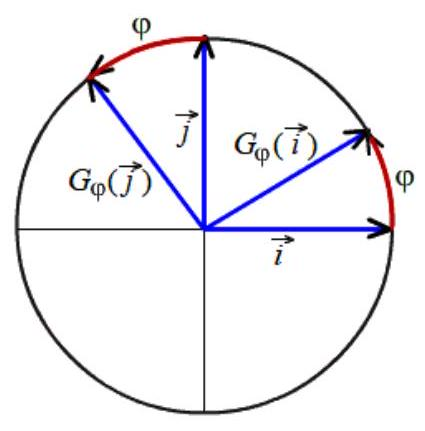
\includegraphics[max width=5cm]{2023_03_20_c2fe6c117849a1a0e8afg-052}
\end{center}

\observacion

Sea V un espacio vectorial euclídeo. $\mathcal{O}(V)$ con la compoición son un grupo denominado grupo ortogonal de $V$. El conjunto $\mathcal{O}^+(V)$ es un subgrupo de $\mathcal{O}(V)$ denominado grupo de giros de $V$. $\mathcal{O}(n,\mathbb{R})$ con el producto de matrices es un grupo y tiene como subgrupo a $\mathcal{O}^+(n, \mathbb{R})$.\\
Si $V$ tiene dimensión finita $n$ y $B$ es una base ortonormal, entonces
$$
\begin{aligned}
	\Phi_B : \mathcal{O}(V) & \longrightarrow \mathcal{O}(n,\mathbb{R}) \\
	f & \longmapsto (f_B)
\end{aligned}
$$
\noindent es un isomorfismo de grupos. Es más, $\Phi_B(\mathcal{O}^+(V)) = \mathcal{O}^+(n, \mathbb{R})$ y $\Phi_B(\mathcal{O}^-(V)) = \mathcal{O}^-(n, \mathbb{R})$. 

\subsubsection{Proposición - Transformacion ortogonal suma}
Sea $V$ un espacio vectorial euclídeo de dimensión finita y sean $U_{1}$ y $U_{2}$ subespacios de $V$ tales que $V=U_{1} \perp U_{2}$. Si $f_{1} \in \mathcal{O}\left(U_{1}\right)$ y $f_{2} \in \mathcal{O}\left(U_{2}\right)$, entonces la aplicación
$$
\begin{aligned}
	f_{1} \perp f_{2}: V & \longrightarrow V \\
	u_1 + u_2 & \longmapsto f_1(u_1) + f_2(u_2)
\end{aligned}
$$
\noindent es una transformación ortogonal de $V$. Si $B$ es ortonormal, entonces
$$
(f_1 \perp f_2)_B = 
\left(\begin{array}{c|c}
	(f_1)_B & 0 \\
	\hline
	0 & (f_2)_B
\end{array}\right)
$$

\demostracion

\noindent Para todo $u_{1}, v_{1} \in U_{1}$ y $u_{2}, v_{2} \in U_{2}$, se tiene

$$
\begin{aligned}
	\left(f_{1} \perp f_{2}\right)\left(u_{1}+u_{2}\right) \cdot\left(f_{1} \perp f_{2}\right)\left(v_{1}+v_{2}\right) & =\left(f_{1}\left(u_{1}\right)+f_{2}\left(u_{2}\right)\right) \cdot\left(f_{1}\left(v_{1}\right)+f_{2}\left(v_{2}\right)\right) \\
	& =f_{1}\left(u_{1}\right) \cdot f_{1}\left(v_{1}\right)+f_{1}\left(u_{1}\right) \cdot f_{2}\left(v_{2}\right) \\
	& +f_{2}\left(u_{2}\right) \cdot f_{1}\left(v_{1}\right)+f_{2}\left(u_{2}\right) \cdot f_{2}\left(v_{2}\right) \\
	& =u_{1} \cdot v_{1}+u_{2} \cdot v_{2}=\left(u_{1}+u_{2}\right) \cdot\left(v_{1}+v_{2}\right) .
\end{aligned}
$$

\subsubsection{Definición - Simetría}
Sea $V$ un espacio vectorial euclídeo de dimensión $n$ y sea $U$ un subespacio vectorial de $V$ ($V = U \perp U^\perp)$. Se llama simetría respecto a $U$ a la transformación ortogonal de $V$
$$
\begin{aligned}
	& S_U : V \Longrightarrow V, \; S_U = \operatorname{Id}_U \perp(-\operatorname{Id})_U \\
	& S_U(v) = S_U(u + w) = u - w, \; u \in U, w \in U^\perp
\end{aligned}
$$
\begin{center}
	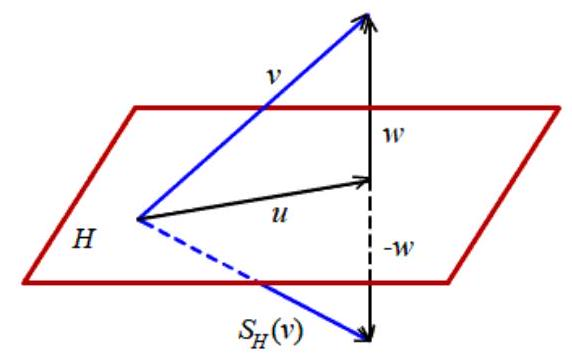
\includegraphics[max width=5cm]{2023_03_20_c2fe6c117849a1a0e8afg-053}
\end{center}
Obsérvese que el conjunto de vectores fijos de $S_{U}$ es $U$ y que $\left(S_{U}\right)^{2}=\mathrm{id}_{V} \Longleftrightarrow S_{U}^{-1}=S_{U}$.

\subsubsection{Proposición - Clasificación de simetrías}
Sea $V$ un espacio vectorial euclídeo de dimensión $n$ y sea $U$ un subespacio vectorial de codimensión $m$ ($\operatorname{dim}_\mathbb{R}U = n - m)$.
\begin{itemize}
	\item Si $m$ es par, entonces $S_U$ es un giro.
	\item Si $m$ es impar, entonces $S_U$ es una reflexión.
\end{itemize}

\demostracion

Dado que $U \perp U^\perp = V$, si $B_U$ es una base ortonormal de $U$ y $B_U$ es una base ortonormal de $U^\perp$, juntándolas se obtiene una base ortonormal de $V$.
\begin{gather*}
	B = \{v_1,\ldots,v_{n-m},\ldots,v_n\} 
	(S_U)_B = (\operatorname{Id}_U \perp (-\operatorname{Id}_{U^\perp}))_B = \operatorname{diag}(1, \ldots, 1, -1, \ldots, -1) 
	\det(S_U) = (-1)^m
	\begin{cases*}
		1 \text{ si m par} \\
		-1 \text{ si m impar}
	\end{cases*}
\end{gather*}

\subsubsection{Corolario - Simetrías en hiperplanos}
Sea $V$ un espacio euclídeo de dimensión finita y $H$ un hiperplano vectorial ($\operatorname{dim}_\mathbb{R}H = n - 1$). Entonces $S_H$ es una reflexión.\\

\ejemplo

Consideremos en $\mathbb{R}^{3}$ el producto escalar usual, esto es, consideremos el espacio euclídeo usual $(\mathbb{R^3}, \cdot)$. Sea $U$ el plano vectorial de $\mathbb{R}^{3}$ cuya ecuación en la base canónica es $U\equiv y-z=0$. Se tiene
$$
U=\langle(1,0,0),(0,1,1)\rangle, \quad U^{\perp}=\{(x, y, z) \in \mathbb{R^3} / x = 0, \; y + z = 0\}=\langle(0,1,-1)\rangle
$$

Sea $B=((1,0,0),(0,1,1),(0,1,-1))$. La simetría respecto al plano vectorial $U$ de $\mathbb{R}^{3}$ es la aplicación lineal $S_{U}=\operatorname{id}_{U} \perp\left(-\operatorname{id}_{U^{\perp}}\right): \mathbb{R}^{3} \rightarrow \mathbb{R}^{3}$ dada por
$$
S_{U}(1,0,0)=(1,0,0), \quad S_{U}(0,1,1)=(0,1,1), \quad S_{U}(0,1,-1)=(0,-1,1)
$$

\noindent luego
$$
\begin{aligned}
	\left(S_{U}\right)_{C}=\left(S_{U}\right)_{B C} \operatorname{(Id)}_{C B} & =\left(\begin{array}{rrr}
		1 & 0 & 0 \\
		0 & 1 & -1 \\
		0 & 1 & 1
	\end{array}\right)\left(\begin{array}{rrr}
		1 & 0 & 0 \\
		0 & 1 & 1 \\
		0 & 1 & -1
	\end{array}\right)^{-1} \\
	& =\left(\begin{array}{rrr}
		1 & 0 & 0 \\
		0 & 1 & -1 \\
		0 & 1 & 1
	\end{array}\right)\left(\begin{array}{rrr}
		1 & 0 & 0 \\
		0 & 1 / 2 & 1 / 2 \\
		0 & 1 / 2 & -1 / 2
	\end{array}\right)=\left(\begin{array}{lll}
		1 & 0 & 0 \\
		0 & 0 & 1 \\
		0 & 1 & 0
	\end{array}\right) .
\end{aligned}
$$

\noindent Así, $S_{U}(x, y, z)=(x, z, y)$

\subsubsection{Proposición - Invarianzas de una transformación ortogonal}
Sea $V$ un espacio vectorial euclídeo de dimensión finita y sea $f$ una transformación ortogonal de $V$ ($f \in \mathcal{O}(V)$). Si $U$ es un subespacio invariante por $f$, entonces también lo es $U^{\perp}$. Recordemos que invariante significa que su imagen está contenida en sí mismo.\\

\demostracion

Veamos que si $f(U) \subset U$, entonces $f\left(U^{\perp}\right) \subset U^{\perp}$. Por ser $f$ un isomorfismo de espacios vectoriales $f(U)=U$ y se tiene que para cada $u \in U$ y cada $w \in U^{\perp}$
$$
u \cdot f(w)=f\left(f^{-1}(u)\right) \cdot f(w)=f^{-1}(u) \cdot w=0 \Longrightarrow f(w) \in U^\perp
$$

\subsubsection{Proposición - Autovalores de las transformaciones ortogonales}
Sea $V$ un espacio vectorial euclídeo de dimensión finita y $f$ una transformación ortogonal de $V$ ($f \in \mathcal{O}(V)$). Si $\lambda \in \mathbb{R}$ es un autovalor de $f$, entonces $\lambda= \pm 1$.\\

\demostracion

Si $v$ es un autovector de $f$ asociado al autovalor $\lambda$, entonces $f(v)=\lambda v$. Se tiene
$$
v \cdot v=f(v) \cdot f(v)=(\lambda v) \cdot(\lambda v)=\lambda^{2} (v \cdot v),
$$

\noindent y dado que $v \neq 0 \Longrightarrow v \cdot v \neq 0$, es $\lambda^{2}=1$.

\subsection{Transformaciones ortogonales del plano vectorial euclídeo}
\subsubsection{Proposición - }
\noindent Si $\mathcal{A} \in \mathcal{O}(2, \mathbb{R})$, entonces
\begin{enumerate}[label=(\arabic*)]
	\item $\displaystyle \mathcal{A} \in \mathcal{O}^{+}(2, \mathbb{R}) \Longleftrightarrow \exists a, b \in \mathbb{R}, a^{2}+b^{2}=1 \mid \mathcal{A}=\left(\begin{array}{rr}
		a & -b \\
		b & a
	\end{array}\right)$
	\item $\displaystyle \mathcal{A} \in \mathcal{O}^{-}(2, \mathbb{R}) \Longleftrightarrow \exists a, b \in \mathbb{R}, a^{2}+b^{2}=1 \mid \mathcal{A}=\left(\begin{array}{rr}
		a & b \\
		b & -a
	\end{array}\right)$
\end{enumerate}

\demostracion
\begin{enumerate}[label=(\arabic*)]
	\item Si
	$$
	\mathcal{A}=\left(\begin{array}{ll}
		a & c \\
		b & d
	\end{array}\right)
	$$
	entonces la condición $\mathcal{A}^{t} \mathcal{A}=I$ es equivalente a las condiciones
	$$
	\begin{cases}
		a^{2}+b^{2}=1, \\ a c+b d=0, \\ c^{2}+d^{2}=1 .
	\end{cases}
	$$
	La condición $\det(\mathcal{A})=1$ equivale a $a d-b c=1$. Resolviendo el sistema
	$$
	\begin{cases}
		a^{2}+b^{2}=1, \\ a c+b d=0, \\ a d-b c=1,
	\end{cases}
	$$
	Separando en casos:
	\begin{align*}
		& a = 0
		\begin{cases}
			b^2 = 1 \\
			bd = 0 \Longrightarrow d = 0 \\
			-bc = 1 \Longrightarrow c = \frac{1}{-b} = -b
		\end{cases} \\
		& a \neq 0
		\begin{cases}
			a^2 + b^2 = 1 \\
			c = \frac{-bd}{a} \Longrightarrow c = -b \\
			ad-bc = 1 \Longrightarrow c = ad + \frac{b^2 d}{a} = 1
		\end{cases}
	\end{align*}
	
	En todo caso, se tiene que $c=-b$ y $d=a$, luego $a^2 d + b^2 d = a \Longrightarrow d = a$
	
	\item Se prueba de forma análoga a (1).
\end{enumerate}

\subsubsection{Proposición - Caracterización de las matrices de giros y reflexiones}
Sea $V$ un plano vectorial euclídeo, $B=\left(v_{1}, v_{2}\right)$ una base ortonormal de $V$ y $f: V \rightarrow V$ una aplicación $\mathbb{R}$-lineal. Se tiene:
\begin{enumerate}[label=(\arabic*)]
	\item $\displaystyle f \in \mathcal{O}^{+}(V) \Longleftrightarrow \exists a, b \in \mathbb{R}, a^{2}+b^{2}=1 \mid f_{B}=\left(\begin{array}{rr}
		a & -b \\
		b & a
	\end{array}\right)$
	\item $\displaystyle f \in \mathcal{O}^{-}(V) \Longleftrightarrow \exists a, b \in \mathbb{R}, a^{2}+b^{2}=1 \mid f_{B}=\left(\begin{array}{rr}
		a & b \\
		b & -a
	\end{array}\right)$
\end{enumerate}

\noindent Además, $a=v_{1} \cdot f\left(v_{1}\right)$.\\

\demostracion 

$$
v_1 \cdot f(v_1) = v_1 \cdot (av_1 + bv_2) = a, \; f_B =
\begin{pmatrix}
	a & * \\
	b & *
\end{pmatrix}
$$

\subsubsection{Proposición - Carácter abeliano de $\mathcal{O}^{+}(2, \mathbb{R})$}
\noindent El grupo $\mathcal{O}^{+}(2, \mathbb{R})$ es abeliano.\\

\demostracion \; (el profe no la hizo)

$$
\left(\begin{array}{rr}
	a & -b \\
	b & a
\end{array}\right)\left(\begin{array}{rr}
	a^{\prime} & -b^{\prime} \\
	b^{\prime} & a^{\prime}
\end{array}\right)=\left(\begin{array}{rr}
	a^{\prime} & -b^{\prime} \\
	b^{\prime} & a^{\prime}
\end{array}\right)\left(\begin{array}{rr}
	a & -b \\
	b & a
\end{array}\right)
$$

\subsubsection{Corolario - Carácter abeliano de $\mathcal{O}^{+}(V)$}
\noindent Si $V$ es un plano vectorial euclídeo, entonces $\mathcal{O}^{+}(V)$ es un grupo abeliano.\\

\demostracion \; (el profe no la hizo)

\noindent Los grupos $\mathcal{O}^{+}(V)$ y $\mathcal{O}^{+}(2, \mathbb{R})$ son isomorfos.

\subsubsection{Proposición - Caracterización de los giros}
Sea $V$ un plano vectorial euclídeo y sean $u$ y $v$ vectores no nulos de $V$ tales que $\|u\|=\|v\| \neq 0$. Existe un único giro $f \in \mathcal{O}^{+}(V)$ tal que $f(u)=v$.\\

\demostracion

Sea $B=\left(v_{1}, v_{2}\right)$ una base ortonormal de $V$ y sean $\left(x_{1}, x_{2}\right),\left(y_{1}, y_{2}\right)$ las coordenadas de $u$ y $v$, respectivamente, en la base $B$. Veamos que existe una matriz ortogonal

$$
A=\left(\begin{array}{rr}
	a & -b \\
	b & a
\end{array}\right)
\; [a^2 + b^2] = 1
$$

tal que
$$
A\left(\begin{array}{l}
	x_{1} \\
	x_{2}
\end{array}\right)=\left(\begin{array}{l}
	y_{1} \\
	y_{2}
\end{array}\right)
$$

Resolviendo el sistema
$$
\begin{cases}
	x_{1} a-x_{2} b=y_{1} \\ x_{2} a+x_{1} b=y_{2}
\end{cases}
\longleftarrow \text{ sistema lineal en $a$ y $b$ }
$$

se tiene que
$$
a=\frac{x_{1} y_{1}+x_{2} y_{2}}{\|u\|^{2}}, \quad b=\frac{x_{1} y_{2}-x_{2} y_{1}}{\|u\|^{2}}, \quad a^{2}+b^{2}=\frac{\|u\|^{2}\|v\|^{2}}{\|u\|^{4}}=1
$$

$A$ es ortogonal ($A^t A = I$) y si definimos $f$ con $(f_B) = A$ es claro que $f(u)=v$.\\

Obsérvese que en un plano vectorial euclídeo un giro está determinado conocida la imagen de un vector no nulo.

\subsubsection{Lema - Propiedad de los giros}
\noindent Sea $V$ un plano vectorial euclídeo, $u$ y $v$ vectores unitarios de $V$ y $f \in \mathcal{O}^{+}(V)$. Se verifica
$$
u \cdot f(u)=v \cdot f(v)
$$

\demostracion

\noindent Sea $g : V \longrightarrow V$ el único giro con $g(u) = v$.
$$
u \cdot f(u)=g(u) \cdot g(f(u)) \overset{g. abel.}{=} g(u) \cdot f(g(u))=v \cdot f(v)
$$

\subsubsection{Definición - Coseno}
Sea $V$ un plano vectorial euclídeo y sea $f$ un giro de $V$ ($f \in \mathcal{O}^+(V)$). Se llama coseno de $f$, y se denota por $\cos f$, al número real
$$
\cos f:=v \cdot f(v)
$$

\noindent donde $v$ es un vector unitario cualquiera de $V$.

\subsubsection{Corolario - Relación entre el coseno y la matriz de un giro}
Sea $V$ un plano vectorial euclídeo y sea $f$ un giro de $V$ ($f \in \mathcal{O}^+(V)$). Sean $B$ y $B^{\prime}$ bases ortonormales de $V$. Si
$$
(f_{B})=\left(\begin{array}{rr}
	a & -b \\
	b & a
\end{array}\right), \quad (f_{B^{\prime}})=\left(\begin{array}{rr}
	a^{\prime} & -b^{\prime} \\
	b^{\prime} & a^{\prime}
\end{array}\right), \quad a^{2}+b^{2}=1, \quad a^{\prime 2}+b^{\prime 2}=1
$$

\noindent entonces $a=a^{\prime}=\cos f$ y $b= b^{\prime}$ o $b= -b^{\prime}$.\\

\demostracion

\noindent Pongamos $B=\left(v_{1}, v_{2}\right)$ y $B^{\prime}=\left(v_{1}^{\prime}, v_{2}^{\prime}\right)$. Ya hemos probado que
$$
a=v_{1} \cdot f\left(v_{1}\right)=\cos f=v_{1}^{\prime} \cdot f\left(v_{1}^{\prime}\right)=a^{\prime}
$$

\noindent Por tanto, $b^{2}=1-a^{2}=1-(a')^2=(b')^{2}$, luego $b= \pm b^{\prime}$.\\

\noindent\underline{Nota}

El valor de $b$ en el corolario anterior depende de la base ortonormal considerada en $V$. Por ejemplo, si $B=\left(v_{1}, v_{2}\right)$ es una base ortonormal de $V$ y

$$
f_{B}=\left(\begin{array}{rr}
	a & -b \\
	b & a
\end{array}\right), \quad a^{2}+b^{2}=1
$$

entonces la matriz asociada a $f$ respecto a $B^{\prime}=\left(v_{2}, v_{1}\right)$ es

$$
f_{B^{\prime}}=\left(\begin{array}{rr}
	a & b \\
	-b & a
\end{array}\right)
$$

\subsection{Orientación}

\subsubsection{Definición - Orientación}
Sea $V$ un espacio vectorial real de dimensión finita. Se dice que las bases $B$ y $B^{\prime}$ ortonormales tienen la misma orientación si el determinante de la matriz de cambio de base $\operatorname{Id}_{BB^{\prime}}$ es positivo ($\operatorname{Id}_{BB'} \in \mathcal{O}(n,\mathbb{R})$). En caso contrario, se dice que tienen distinta orientación.

La relación ''tener la misma orientación'' en el conjunto de bases de $V$ es una relación de equivalencia.
\begin{itemize}
	\item Reflexiva: $\det(\operatorname{Id}_{BB}) = 1$.
	\item Simétrica: $\det(\operatorname{Id}_{B'B}) = \det(\operatorname{Id}_{BB'})^{-1} = 1^{-1} = 1$
	\item Transitiva. Sean $B$ y $B'$ bases ortonormales con la misma orientación. Sea también $B''$ tal que tiene la misma orientación que $B'$. Entonces:
	$$
	\det(\operatorname{Id}_{BB''}) = \det((\operatorname{Id}_{B'B''})(\operatorname{Id}_{BB'})) = \det(\operatorname{Id}_{B'B''})\det(\operatorname{Id}_{BB'}) = 1
	$$ 
\end{itemize}
\noindent Existen solamente dos clases de equivalencia distintas para esta relación. Si $B'$ tiene diferente orientación a $B$ y $B''$ tiene diferente orientación a $B$, entonces $B'$ y $B''$ tienen la misma orientación.
$$
\det(\operatorname{Id}_{B'B''}) = \det(\operatorname{Id}_{BB''})\det(\operatorname{Id}_{B'B}) = 1
$$
Si $B$ es una base de $V$, la clase de equivalencia $[B]$ se dice que es una orientación en $V$. Tomamos una base $B$ y todas las de su clase de equivalencia y le llamamos \underline{orientación positiva}.
\begin{gather*}
	B = (v_1,\ldots,v_i,\ldots,v_j,\ldots,v_n) \text{ tiene orientación positiva} \\
	\Longleftrightarrow B' = (v_1,\ldots,v_j,\ldots,v_i,\ldots,v_n) \text{ tiene orientación negativa}
\end{gather*}

El par $(V,[B])$ se llama espacio vectorial orientado. Diremos que $V$ está orientado con la base $B$ para indicar que consideramos $(V,[B])$ y en este caso las bases de $[B]$ se dice que son bases de orientación positiva y las bases de $V$ que no están en $[B]$ se dice que son bases de orientación negativa.

Consideramos que $\mathbb{R}^{n}$ está orientado con la base canónica.

\ejemplos
\begin{enumerate}[label=(\arabic*)]
	\item El espacio $V_{2}$ de los vectores libres del plano se considera orientado con la base ortonormal $C=$ $(\vec{i}, \vec{j})$ asociada a la referencia canónica $\mathcal{C}=\left\{E_{1}, E_{2} ; O\right\}$ del plano ordinario.
	
	\item El espacio $V_{3}$ de los vectores libres del espacio se considera orientado con la base ortonormal $C=(\vec{i}, \vec{j}, \vec{k})$ asociada a la referencia canónica $\mathcal{C}=\left\{E_{1}, E_{2}, E_{3} ; O\right\}$ del espacio ordinario.
	
	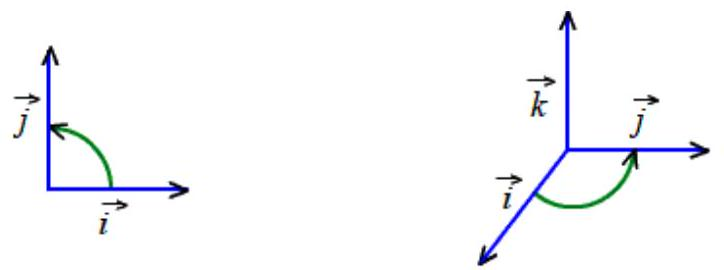
\includegraphics[max width=7cm, center]{2023_03_20_c2fe6c117849a1a0e8afg-057}
\end{enumerate}

\subsubsection{Proposición - Orientaciones y matrices de giros}
Sea $V$ un plano vectorial euclídeo y sea $f$ un giro de $V$ ($f \in \mathcal{O}^+(V)$). Sean $B$ y $B^{\prime}$ son bases ortonormales de $V$. Entonces:
$$
f_{B}=\left(\begin{array}{rr}
	a & -b \\
	b & a
\end{array}\right), \quad f_{B^{\prime}}=\left(\begin{array}{rr}
	a & -b^{\prime} \\
	b^{\prime} & a
\end{array}\right), \quad a = \operatorname{cos}f
$$
Si $B$ y $B^{\prime}$ tienen la misma orientación, entonces $b = b'$. Si $B$ y $B^{\prime}$ tienen distinta orientación, entonces $b = -b'$.

\demostracion

Si $B$ y $B'$ tienen la misma orientación, entonces
\begin{gather*}
	(\operatorname{Id}_{BB'}),(\operatorname{Id}_{B'B}) \in \mathcal{O}^+(2,\mathbb{R}) \\
	(f_{B'}) = (\operatorname{Id}_{BB'})(f_{B})(\operatorname{Id}_{B'B})
	= (\operatorname{Id}_{BB'})(\operatorname{Id}_{B'B})(f_B)
\end{gather*}

Si $B=\left(v_{1}, v_{2}\right)$ y las bases $B$ y $B^{\prime}$ tienen distinta orientación, entonces las bases $B^{\prime \prime}=\left(v_{2}, v_{1}\right)$ y $B^{\prime}$ tienen igual orientación. Por tanto,

$$
f_{B^{\prime}}=f_{B^{\prime \prime}}=\left(\begin{array}{rr}
	a & b \\
	-b & a
\end{array}\right)
$$

\subsubsection{Proposición - Isomorfismo entre $\displaystyle R: \frac{\mathbb{R}}{2 \pi \mathbb{Z}}$ y $\mathcal{O}^{+}(2, \mathbb{R})$}
\noindent Se tiene el isomorfismo de grupos:
$$
\begin{gathered}
	R: \frac{\mathbb{R}}{2 \pi \mathbb{Z}} \longrightarrow \mathcal{O}^{+}(2, \mathbb{R}) \\
	[\varphi] = \varphi+2 \pi \mathbb{Z} \longmapsto R_{\varphi} := \begin{pmatrix}
		\operatorname{cos}\varphi & -\operatorname{sen}\varphi \\
		\operatorname{sen}\varphi & \operatorname{cos}\varphi
	\end{pmatrix}
\end{gathered}
$$
\demostracion
\begin{enumerate}[label=(\arabic*)]
	\item Bien definido ya que \textit{sen} y \textit{cos} tienen periodo $2\pi$
	$$
	R_\varphi R_\varphi^t = \operatorname{Id}
	$$
	\item R es biyectiva, pues si $a^2 + b^2 = 1$, entonces $(a,b)$ pertenece a la circunferencia unitaria ya que se parametriza por $\varphi \Longrightarrow (\operatorname{cos}\varphi, \operatorname{sen}\varphi) = (a,b)$, bien definida con $\varphi \in [0,2\pi)$.
	\item Es homomorfismo de grupos
	\begin{gather*}
		R_\varphi R_\varphi =
		\begin{pmatrix}
			\operatorname{cos}\varphi & -\operatorname{sen}\varphi \\
			\operatorname{sen}\varphi & \operatorname{cos}\varphi
		\end{pmatrix}
		\begin{pmatrix}
			\operatorname{cos}\varphi & -\operatorname{sen}\varphi \\
			\operatorname{sen}\varphi & \operatorname{cos}\varphi
		\end{pmatrix} \\ =
		\begin{pmatrix}
			-\operatorname{cos}\varphi\operatorname{sen}\varphi & -\operatorname{sen}\varphi\operatorname{cos}\varphi \\
			-\operatorname{sen}\varphi\operatorname{sen}\varphi & \operatorname{cos}\varphi\operatorname{cos}\varphi
		\end{pmatrix} = 
		\begin{pmatrix}
			\operatorname{cos}(\varphi + \varphi) & -\operatorname{sen}(\varphi + \varphi) \\
			\operatorname{sen}(\varphi + \varphi) & \operatorname{cos}(\varphi + \varphi)
		\end{pmatrix}
	\end{gather*}
\end{enumerate}

\subsubsection{Definición - Giro de ángulo orientado}
Sea $V$ un plano vectorial euclídeo orientado y $\varphi \in[0,2 \pi)$. Se llama giro de ángulo orientado $\varphi+2 \pi \mathbb{Z}$, o también giro de ángulo orientado $\varphi$, al giro $G_{\varphi}: V \rightarrow V$ cuya matriz asociada respecto a cualquier base ortonormal de $V$ de orientación positiva es
$$
\left(G_{\varphi}\right)_{B}=R_{\varphi}=\left(\begin{array}{rr}
	\cos \varphi & -\operatorname{sen} \varphi \\
	\operatorname{sen} \varphi & \cos \varphi
\end{array}\right)
$$
Dado que no depende de la base y todas las matrices de $\mathcal{O}^+(2,\mathbb{R})$ son de ésta forma, estos son todos los posibles giros de $\mathcal{O}^+(V)$. Además, si $f \in \mathcal{O}^+(V)$ y $f = G_\varphi$, se define el seno de f como $\operatorname{sen}f = \operatorname{sen}\varphi$. Por tanto, si $f \in \mathcal{O}^+(V)$ y $B$ es ortonormal de orientación positiva,
$$
(f_B) =
\begin{pmatrix}
	\operatorname{cos}\varphi & -\operatorname{sen}\varphi \\
	\operatorname{sen}\varphi & \operatorname{cos}\varphi
\end{pmatrix}
$$

\subsection{Clasificación de las transformaciones ortogonales en el plano}

\subsubsection{Teorema - Clasificación de las transformaciones ortogonales en el plano}
\noindent Sea $V$ un plano vectorial euclídeo y $f \in \mathcal{O}(V)$. 
\begin{enumerate}[label=(\arabic*)]
	\item Si $f \in \mathcal{O}^+(V)$ y $B$ es una base ortonormal de $V$ tal que
	$$
	(f_B) =
	\begin{pmatrix}
		a & -b \\
		b & a
	\end{pmatrix}
	\text{ con } a^2 + b^2 = 1
	$$
	entonces las raíces del polinomio característico de $f$ son $a \pm bi$ y $\operatorname{cos}f = a$. En particular, si $b = 0$:
	\begin{itemize}
		\item $a = 1, \; f = \operatorname{Id}_V$ y por tanto el giro de ángulo $0$.
		\item $a = -1, \; f = -\operatorname{Id}_V$ y por tanto el giro de ángulo $\pi$.
	\end{itemize}
	(Son los casos de $\lambda = 1$ doble y $\lambda = -1$ doble).
	
	\item Si $f \in \mathcal{O}^-(V)$, entonces $f$ tiene los autovalores $1$ y $-1$; en este caso existe una base ortonormal $B$ de $V$ tal que
	$$
	(f_B) = \begin{pmatrix}
		1 & 0 \\
		0 & -1
	\end{pmatrix}
	$$
	y por tanto $f = S_{V_1}, \; V_1 = \operatorname{Ker}(f - \operatorname{Id_V})$.
\end{enumerate}
\demostracion
\begin{enumerate}[label=(\arabic*)]
	\item $\displaystyle P_f(x) = \begin{vmatrix}
		a - x & - b \\
		b & a - x
	\end{vmatrix} = (a - x)^2 = b^2 = x^2 - 2ax + a^2 + b^2 = x^2 - 2ax + 1 = 0 \Longleftrightarrow x = \frac{2a \pm \sqrt{4a^2 - 4}}{2} = a \pm \sqrt{a^2 - 1} = a \pm \sqrt{-b^2} = a \pm bi$.
	
	Si $b = 0$ y $a = 1 \Longrightarrow (f_B) = \begin{pmatrix}
		1 & 0 \\
		0 & 1
	\end{pmatrix} \Longrightarrow f = \operatorname{Id}_V$.
	
	Si $b = 0$ y $a = -1 \Longrightarrow (f_B) = \begin{pmatrix}
		-1 & 0 \\
		0 & -1
	\end{pmatrix} \Longrightarrow f = -\operatorname{Id}_V$.
	
	Si $V$ está orientado y $B$ tiene orientación positiva, entonces $f$ es el giro de ángulo $\varphi$ con $\operatorname{cos}\varphi = a$ y $\operatorname{sen}\varphi = b$.
	
	\item Si $f \in \mathcal{O}^-(V)$, entonces dada $B'$ base ortonormal sabemos que
	$$
	(f_{B'}) = \begin{pmatrix}
		a & b \\
		b & -a
	\end{pmatrix}, \quad a^2 + b^2 = 1
	$$
	Por tanto
	\begin{gather*}
		P_f(x) = \begin{vmatrix}
			a - x & b \\
			b & - a - x
		\end{vmatrix} = x^2 - a^2 - b^2 = x^2 - 1 = 0 \Longleftrightarrow \\
		\Longleftrightarrow x = 1 \text{ o } x = -1
	\end{gather*}
	Sea $v \neq 0$ vector propio de $\lambda = 1$.
	Sea $w \neq 0$ vector propio de $\lambda = -1$.
	Veamos que $v$ y $w$ son ortogonales
	$$
	v \cdot w = f(v) \cdot f(w) = v \cdot (-w) = - v \cdot w \Longrightarrow 2(v \cdot w) = 0 \Longrightarrow v \cdot w = 0
	$$
	Si tomamos $v_1 = \frac{v}{\|v\|}$ y $v_2 = \frac{w}{\|w|}$ entones $B = (v_1, v_2)$ es una base ortonormal y
	$$
	(f_b) = \begin{pmatrix}
		1 & 0 \\
		0 & -1
	\end{pmatrix}
	$$
	Por tanto
	$$
	f = \operatorname{Id}_{V_1} \perp (-\operatorname{Id}_{V_1}) = \operatorname{Id}_{V_1} \perp (-\operatorname{Id}_{V_1^\perp}) = S_{V_1}
	$$
\end{enumerate}

\subsubsection{Corolario - Clasificación}
\begin{enumerate}[label=(\arabic*)]
	\item Toda transformación ortogonal cuyo polinomio característico  no tiene raíces reales es un giro.
	\item Toda reflexión es una simetría.
	\item Las transformaciones ortogonales de $V$ son giros o simetrías con respecto a un subespacio de dimensión $1$.
\end{enumerate}

\subsubsection{Corolario - Clasificación}
\noindent Sea $V$ un plano euclídeo y $f \in \mathcal{O}(V)$.
\begin{enumerate}[label=(\arabic*)]
	\item Si el único vector fijo de $f$ es el vector $0$, entonces $f$ es un giro y $f \neq \operatorname{Id}_V$.
	\item Si $f$ tiene un solo subespacio de vectores fijos de dimensión $1$, entonces $f$ es la simetría con respecto ese subespacio.
\end{enumerate}

\subsection{Clasificación de las transformaciones ortogonales en el espacio vectorial euclídeo tridimensional}

\subsubsection{Definición - Giro con eje}
Sea $V$ un espacio vectorial euclídeo tridimensional. Se define el giro de eje $U = \langle w \rangle, \; w \neq 0$, como
$$
f = f_1 \perp \operatorname{Id}_{\langle w \rangle} \text{ donde } f_1 \in \mathcal{O}^+(\langle w \rangle^\perp)
$$

\subsubsection{Definición - Eje orientado}
Sea $V$ un espacio vectorial euclídeo. Sea $w \in W, \; w \neq 0$. Se llama eje orientado al subespacio vectorial $\langle w \rangle$ donde tomamos la orientación en la cual una base de orientación positiva es $\displaystyle B = \left\{ \frac{w}{\|w\|} \right\}$.

\subsubsection{Proposición - Un eje orientado induce una orientación}
Sea $V$ un espacio vectorial euclídeo tridimensional orientado. Tomemos un eje orientado $\langle w \rangle$, podemos considerar $\|w\| = 1$. Entonces, $\langle w \rangle$ induce una orientación en el plano vectorial $\langle w \rangle^\perp$ dada por considerar una base ortonormal $B_1 = (u,v)$ en el plano $\langle w \rangle^\perp$ tal que $B = (u,v,w)$ es de orientación positiva en $V$.

\demostracion

Veamos que la orientacion de $\langle w \rangle^\perp$ está bien definida. Sea $B_1' = (u',v')$ base ortonormal de $\langle w \rangle^\perp$ verificando que $B' = (u',v',w)$ tiene orientación positiva. Veamos que $B_1$ y $B_1'$ tiene la misma orientación.

Como $B$ y $B'$ tienen orientación positiva, sabemos que $\det(I_{BB'}^V) = 1$.
$$
\text{Si }\operatorname{Id}_{B_1 B_1'}^{\langle w \rangle^\perp} = \begin{pmatrix}
	a & c \\
	b & d
\end{pmatrix} \text{ entonces } \operatorname{Id}_{BB'}^V = \begin{pmatrix}
	a & c & 0 \\
	b & d & 0 \\
	0 & 0 & 1
\end{pmatrix}
$$
y por tanto
$$
\det\left(\operatorname{Id}_{B_1 B_1'}^{\langle w \rangle^\perp}\right) = \det\left(\operatorname{Id}_{B_1 B_1'}^V\right) = 1
$$ 
Por lo que $B_1$ y $B_1'$ tiene la misma orientación.

\subsubsection{Definición - Giro de eje orientado y ángulo}
Sea $V$ un espacio vectorial euclídeo tridimensional orientado y $w \in V - \{0\}$. Se llama giro de eje orientado $\langle w \rangle$ y ángulo $\varphi$ a la transformación ortogonal
$$
G_{\langle w \rangle, \varphi} = G_\varphi \perp \operatorname{Id}_{\langle w \rangle}
$$
donde el plano $\langle w \rangle^\perp$ tiene la orientación inducida por $\langle w \rangle$ y $G_\varphi \in \mathcal{O}^+ (\langle w \rangle^\perp)$.

\observacion

$G_{\langle w \rangle, \varphi} \in \mathcal{O}^+(V)$

\subsubsection{Proposición - Existencia de un eje invariante en los giros tridimensionales}
Sea $V$ un espacio vectorial euclídeo tridimensional y $f \in \mathcal{O}(V)$. Entonces, $\exists v \in V - \{0\}$ tal que $f = f_1 \perp \operatorname{Id}_{\langle v \rangle}$ o $f = f_1 \perp -(\operatorname{Id}_{\langle v \rangle})$, donde $f_1 \in \mathcal{O}(\langle v \rangle^\perp)$.

\noindent\underline{Demostracion}

$P_f(x)$ tiene al menos una raíz real $\lambda$ (ya que tiene grado $3$). Por tanto, hemos visto, $\lambda = 1$ o $\lambda = -1$. Sea $v \neq 0$ vector propio de $\lambda$. Es inmediato que $f(\langle v \rangle) = \langle v \rangle$, y por tanto $f(\langle v \rangle)^\perp = \langle v \rangle^\perp$. Podemos definir
$$
f_1 = f|_{\langle v \rangle^\perp} : \langle v \rangle^\perp \longrightarrow \langle v \rangle^\perp
$$
entonces, al ser una restricción de una isometría, es una isometría. Por tanto, $f_1 \in \mathcal{O}(\langle v \rangle^\perp)$. Como $V = \langle v \rangle^\perp \perp \langle v \rangle$,
$$\begin{cases}
	f = f_1 \perp \operatorname{Id}_{\langle v \rangle} \\
	o \\
	f = f_1 \perp \operatorname{Id}_{\langle v \rangle}
\end{cases}
$$
\ejemplo

\noindent $(\mathbb{R}^3, \cdot)$ espacio euclídeo usual. El giro de eje orientado $\langle (0, 1, 1) \rangle$ y ángulo $\displaystyle \frac{2\pi}{3}$. La base 
$$
\displaystyle B_1 = \left(\left(1,0,0\right),\left(0, \frac{\sqrt{2}}{2},-\frac{\sqrt{2}}{2}\right)\right)
$$
es una base de orientación positiva de $\langle(0,1,1)\rangle^\perp = \langle (1,0,0),(0,1,-1)\rangle$, ya que 
$$
B = \left(\left(1,0,0\right),\left(0, \frac{\sqrt{2}}{2},-\frac{\sqrt{2}}{2}\right),\left(0, \frac{\sqrt{2}}{2},\frac{\sqrt{2}}{2}\right)\right)
$$
es de orientación positiva
$$
\det\left(\operatorname{Id}_{B\mathcal{C}}\right) = \begin{vmatrix}
	1 & 0 & 0 \\
	0 & \frac{\sqrt{2}}{2} & \frac{\sqrt{2}}{2} \\
	0 & -\frac{\sqrt{2}}{2} & \frac{\sqrt{2}}{2}
\end{vmatrix} = 1
$$
Se puede hacer el giro
$$
\left(G_{\frac{2\pi}{3}}\right) = \begin{pmatrix}
	-\frac{1}{2} & -\frac{\sqrt{3}}{2} \\
	\frac{\sqrt{3}}{2} & -\frac{1}{2}
\end{pmatrix}
$$
Así
$\left(G_{\langle (0,1,1) \rangle, \frac{2\pi}{3}}\right)_B = \begin{pmatrix}
	-\frac{1}{2} & -\frac{\sqrt{3}}{2} & 0 \\
	\frac{\sqrt{3}}{2} & -\frac{1}{2} & 0 \\
	0 & 0 & 1
\end{pmatrix}$

\subsubsection{Teorema - Clasificación de las transformaciones ortogonales en el espacio vectorial euclídeo tridimensional}
Sea $V$ un espacio afín euclídeo tridimensional (orientado) y sea $f \in \mathcal{O}(V)$. $V_1 = \ker (f-\operatorname{Id}_V)$, $V_{-1} = \ker (f+\operatorname{Id}_V)$.
\begin{enumerate}[label=(\arabic*)]
	\item Si $f \in \mathcal{O}^+(V)$ y $f \neq \operatorname{Id}_V$, entonces $f$ es un giro de eje $V_1$ ($\operatorname{Id}_V$ es un giro de ángulo $0$ en cualquier eje).
	\item Si $f \in \mathcal{O}^-(V)$ y $f = -\operatorname{Id}_V$ o $f$ es la simetría con respecto al plano vectorial $V_1$ o $f$ es la composición de un giro de eje $V_{-1}$ y la simetría respecto el plano vectorial $(V_{-1})^\perp$.
\end{enumerate}
\demostracion

Dado $f \in \mathcal{O}(V)$ existe $v \in V-\{0\}$ tal que $f 
= f_1 \perp \operatorname{Id}_{\langle v \rangle^\perp}$ o $f = f_1 \perp (-\operatorname{Id}_{\langle v \rangle})$ donde $f_1 \in \mathcal{O}(\langle v \rangle^\perp)$. Consideremos $B_1 = (v_1, v_2)$ una base ortonormal de $\langle v \rangle^\perp$ y tomemos $B = (v_1,v_2,v_3)$ con $\displaystyle v_3 = \frac{v}{\|v\|}$ base ortonormal de $V$. Tenemos 4 casos.
\begin{enumerate}[label=(\arabic*)]
	\item $f = f_1 \perp \operatorname{Id}_{\langle v_3 \rangle}$ con $f_1 \in \mathcal{O}^+(\langle v_3 \rangle)^\perp$. Se tiene que
	$$
	\left(f_1\right)_{B_1} = \begin{pmatrix}
		a & -b \\
		b & a
	\end{pmatrix} \text{ con } a^2 + b^2 = 1
	$$
	Por tanto, $\displaystyle \left(f_B\right) = \begin{pmatrix}
		a & -b & 0 \\
		b & a & 0 \\
		0 & 0 & 1
	\end{pmatrix}$. Es claro que $f \in \mathcal{O}^+(V)$.
	
	Si $a = 1 \Longrightarrow b = 0$ y $\displaystyle \left(f_B\right) = \begin{pmatrix}
		1 & 0 & 0 \\
		0 & 1 & 0 \\
		0 & 0 & 1
	\end{pmatrix} \Longrightarrow f = \operatorname{Id}_V$ y $\lambda = 1$ es un autovalor triple.
	
	Si $a \neq q$, entonces los autovalores son $1$ y $a \pm b \i = 1$. En particular,
	$$
	b = 0 \Longrightarrow a = -1 \Longrightarrow \left(f_B\right) = \begin{pmatrix}
		-1 & 0 & 0 \\
		0 & -1 & 0 \\
		0 & 0 & -1
	\end{pmatrix}
	$$
	es el giro de eje $V_1 = \langle v_3 \rangle$ y ángulo $\pi$ (Es el caso de $\lambda = 1$ simple y $\lambda = -1$ doble) (puede que el $V_1$ sea un $V_{-1}$, no entendía la letra xd). $f$ es un giro de eje orientado $\langle v_3 \rangle = V_1$ y ángulo $\varphi$. Si $B$ tiene orientación positiva $\varphi$ es tal que $\cos \varphi = a$ y $\sin \varphi = b$.
	
	\item $f = f_1 \perp \operatorname{Id}_{\langle v_3 \rangle}$ y $f_1 \in \mathcal{O}^-(\langle v_3 \rangle^\perp)$. Sea $B_1' = (v_1', v_2')$ la base ortonormal de $\langle v_3 \rangle$, donde
	$$
	\left(f_1\right)_{B_1'} = \begin{pmatrix}
		1 & 0 \\
		0 & -1
	\end{pmatrix}
	$$
	Pongamos $B' = (v_1',v_2',v_3')$. Entonces,
	$$
	\left(f_{B'}\right) = \begin{pmatrix}
		1 & 0 & 0 \\
		0 & -1 & 0 \\
		0 & 0 & 1
	\end{pmatrix} \quad \begin{pmatrix}
		\lambda = 1 \text{ doble} \\
		\lambda = -1 \text{ simple}
	\end{pmatrix}
	$$
	$f = \operatorname{Id}_{\langle v_1',v3 \rangle} \perp (-\operatorname{Id}_{\langle v_2' \rangle}) = S_{V_1} \in \mathcal{O}^-(V)$.
	
	\item $f = f_1 \perp (-\operatorname{Id}_{\langle v_3 \rangle})$ y $f_1 \in \mathcal{O}^+(\langle v_3 \rangle^\perp)$. $f \in \mathcal{O}^-(V)$. Sabemos que
	$$
	(f)_{B_1} = \begin{pmatrix}
		a & -b \\
		b & a
	\end{pmatrix} \quad a^2 + b^2 = 1
	$$
	Y por tanto $\displaystyle (f_B) = \begin{pmatrix}
		a & -b & 0 \\
		b & a & 0 \\
		0 & 0 & -1
	\end{pmatrix}$.
	Si $\displaystyle a = 1 \Longrightarrow b = 0 \Longrightarrow (f_B) = \begin{pmatrix}
		1 & 0 & 0 \\
		0 & 1 & 0 \\
		0 & 0 & -1
	\end{pmatrix} \Longrightarrow f = S_{V_1}$.
	Si $\displaystyle a = -1 \Longrightarrow b = 0 \Longrightarrow (f_B) = \begin{pmatrix}
		-1 & 0 & 0 \\
		0 & -1 & 0 \\
		0 & 0 & -1
	\end{pmatrix} \Longrightarrow f = -\operatorname{Id}_V$.
	Si $b \neq 0$, entones las raíces del polinomio característico de $f$ son $-1$ y $-1 \neq a \pm b \neq 1$, teniendo en cuenta que
	$$
	\begin{pmatrix}
		a & -b & 0 \\
		b & a & 0 \\
		0 & 0 & -1
	\end{pmatrix} = \begin{pmatrix}
		1 & 0 & 0 \\
		0 & 1 & 0 \\
		0 & 0 & -1
	\end{pmatrix} \begin{pmatrix}
		a & -b & 0 \\
		b & a & 0 \\
		0 & 0 & 1
	\end{pmatrix}
	$$
	entonces $f$ es la composición de un giro de eje orientado $V_{-1} = \langle v_3 \rangle$ con la simetría con respecto $\langle v_1, v_2 \rangle = (V_{-1})^\perp$.
	
	\item $f = f_1 \perp (-\operatorname{Id}_{\langle v_3 \rangle})$ y $f_1 \in \mathcal{O}^-(\langle v_3 \rangle^\perp)$. $f \in \mathcal{O}^+(V)$. Sea $B_1' = (v_1',v_2')$ base ortonormal de $\langle v_3 \rangle^\perp$ tal que 
	$$
	\left(f_1\right)_{B_1'} = \begin{pmatrix}
		1 & 0 \\
		0 & -1
	\end{pmatrix}
	$$
	Entonces,
	$$
	\left(f_{B'}\right) = \begin{pmatrix}
		1 & 0 & 0 \\
		0 & -1 & 0 \\
		0 & 0 & -1
	\end{pmatrix} \quad \begin{pmatrix}
		\lambda = 1 \text{ doble} \\
		\lambda = -1 \text{ simple}
	\end{pmatrix}
	$$
	es el giro de eje $\langle v_1' \rangle = V_1$ y $\pi$ grados.
\end{enumerate}

\subsubsection{Corolario - Clasificación}
\noindent Sea $V$ espacio vectorial euclídeo orientado tridimensional y $f \in \mathcal{O}(V)$.
\begin{enumerate}[label=(\arabic*)]
	\item Si $1$ es autovalor de $f$ de multiplicidad $1$ y las otras dos raíces del polinomio característico son $a \pm bi \neq 1, \; a^2 + b^2 = 1$, entonces $f$ es un giro de eje orientado $V_1$ y ángulo $\varphi$ (que depende de la orientación del eje) donde $\cos \varphi = a$ y $\sin \varphi = b$. Además, $\lambda = 1$ es triple y $f = \operatorname{Id}_V$ es un giro de $0$ grados en cualquier eje.
	
	\item Si $1$ es autovalor de $f$ con multiplicidad $2$ entonces $f$ es la simetría respecto al plano vectorial $V_1$.
	
	\item Si $-1$ es un autovalor de multiplicidad $1$ y las otras dos raíces del polinomio característico de $f$ son $a \pm bi \neq \pm 1$, entonces $f$ es la composición de un giro de eje orientado $V_1$ y ángulo $\varphi$ (que depende de la orientación de $V_1$) tal que $\cos \varphi = a$ y $\sin \varphi = b$, y la simetría con respecto al plano $(v_{-1})^\perp$.
	
	\item Si $-1$ es triple, entonces $f$ es la simetría con respecto al origen ($f = -\operatorname{Id}_V$).
	$$
	S_{\{0\}} = \operatorname{Id}_{\{0\}} \perp -(\operatorname{Id})_{\{0\}^\perp} = -\operatorname{Id}_V
	$$
\end{enumerate}

\subsubsection{Corolario - Clasificación}
Sea $V$ espacio vectorial euclídeo orientado tridimensional y $f \in \mathcal{O}(V)$.
\begin{enumerate}[label=(\arabic*)]
	\item Si $f$ tiene solo un subespacio de vectores fijos de dimensión $1$, entones $f$ es un giro con respecto ese eje.
	\item Si $f$ tiene únicamente un subespacio de vectores fijos de dimensión $2$, entonces $f$ es la simetría respecto ese subespacio.
	\item Si el único vector fijo de $f \neq -\operatorname{Id}_V$ es el vector cero, entonces $f$ es la composición de un giro con una simetría respecto a un plano vectorial (donde el eje de giro y el plano son ortogonales).
\end{enumerate}

\newpage

\section{Tema 3: Espacios afines euclídeos}

\subsection{Introducción a los espacios afines euclídeos}

\subsubsection{Definición - Espacio afín euclídeo}
Un espacio afín $\mathbb{A}$ sobre $V$ se dice espacio afín euclídeo si $V$ es un espacio vectorial euclídeo.

\subsubsection{Definición - Distancia}
Sean $P,Q \in \mathbb{A}$ espacio afín euclídeo. Se define la distancia de $P$ a $Q$ como
$$
\operatorname{d}(P,Q) := \|\overrightarrow{PQ}\|
$$

\subsubsection{Propiedades de la distancia}
\begin{enumerate}[label=(\arabic*)]
	\item $\operatorname{d}(P,Q) \ge 0, \; \forall P,Q \in \mathbb{A}$.
	\item $\operatorname{d}(P,Q) = 0 \Longleftrightarrow P = Q$.
	\item $\operatorname{d}(P,Q) \le \operatorname{d}(P,R) + \operatorname{d}(R,Q) \text{ con } P,Q,R \in \mathbb{A}$.
	\item $\distancia{P,Q} = \distancia{Q,P}$.
	\item Teorema de Pitágoras. $\overrightarrow{P,Q} \cdot \overrightarrow{P,R} = 0 \Longleftrightarrow \distancia{P,Q}^2 = \distancia{P,R}^2 + \distancia{R,Q}^2$.
\end{enumerate}

\subsubsection{Definición - Referencia rectangular}
Sea $\mathbb{A}$ un espacio afín euclídeo de dimensión finita. Una referencia $\mathcal{R} = \{P_1,\ldots,P_n;Q\}$ se dice referencia rectangular si $B_\mathcal{R}$ es ortonormal.

\subsubsection{Proposicion}
Sea $\mathcal{R} = \{P_1,\ldots,P_n;Q\}$ una referencia rectangular de $\mathbb{A}$. Sean $P = (x_1, \ldots, x_n)_\mathcal{R}$ y $P' = (y_1, \ldots, y_n)_\mathcal{R}$ puntos de $\mathbb{A}$. Entonces,
$$
\distancia{P,P'} = \sqrt{\sum_{i = 1}^{n} (y_i - x_i)^2}
$$
\demostracion
$$
\distancia{P,P'} = \| \overrightarrow{PP'} \| = \|\overrightarrow{PQ} + \overrightarrow{QP}\| = \|\overrightarrow{QP'} - \overrightarrow{QP}\| = \sqrt{\sum_{i = 1}^{n}(y_i - x_i)^2}
$$
con $y_i - x_i$ en base $B_\mathcal{R}$ ortonormal.

\subsubsection{Definición - Variedades lineales perpendiculares}
Se dice que las variedades lineales $L_1 = A + V_1$ y $L_2 = B + V_2$ (de un espacio afín euclídeo) son perpendiculares si $V_1 \perp V_2$ (ortogonales).

\subsection{Proyección ortogonal de un punto sobre una variedad lineal}

\subsubsection{Definición - Variedad lineal perpendicular}
Sea $\mathbb{A}$ un espacio afín euclídeo. Sea $L = A + U$ una variedad lineal y $P \in \mathbb{A}$. Entonces se denomina variedad lineal perpendicular a $L$ que pasa por $P$ a $L_P^\perp = P + U^\perp$.

\subsubsection{Proposición}
Sea $\mathbb{A}$ espacio afín euclídeo de dimensión finita. Entonces $L = A + U$ y $L_P^\perp$ se cortan en un único punto.

\demostracion

Por ser $V$ un espacio vectorial euclídeo de dimensión finita, $V = U \perp U^\perp$. Tomemos
$$
\overrightarrow{AP} \in V = U \perp U^\perp = U \oplus U^\perp \Longrightarrow L \cap L_P^\perp \neq \varnothing
$$
Entonces,
\begin{gather*}
\dim(L \cap L_P^\perp) = \dim(L) + \dim(L_P^\perp) - \dim(L \circ L_P^\perp) = \dim_\mathbb{R}U + \dim_\mathbb{R}U - \dim_\mathbb{R}(U \oplus U^\perp) = \\ = \dim_\mathbb{R} U + \dim_\mathbb{R} U^\perp - \dim_\mathbb{R} U - \dim_\mathbb{R} U' = 0
\end{gather*}

\subsubsection{Definición - Proyección ortogonal}
Sea $\mathbb{A}$ un espacio afín euclídeo de dimensión finita. Sean $P \in \mathbb{A}$ y $L = A + U$ una variedad de $\mathbb{A}$. $P_0 = L \cap L_P^\perp$.

\observacion

En las hipótesis anteriores se tiene que
$$
\begin{array}{r}
	\overrightarrow{AP_0} \in U \\
	\overrightarrow{PP_0} \in U^\perp
\end{array} \Longrightarrow \overrightarrow{AP_0} \perp \overrightarrow{PP_0}
$$

\subsection{Distancia entre variedades lineales}

\subsubsection{Definición - Distancia entre variedades lineales}
Sean $L_1, L_2$ variedades lineales de un espacio afín euclídeo $\mathbb{A}$. Se define la distancia de $L_1$ a $L_2$ como
$$
\distancia{L_1,L_2} := \inf \left\{\distancia{P,Q} \,/\, P \in L_1, Q \in L_2\right\}
$$

\subsubsection{Proposición}
Sea $\mathbb{A}$ y $L_1, L_2$ variedades lineales de $\mathbb{A}$. Entonces,
$$
L_1 \cap L_2 \neq \varnothing \Longleftrightarrow \distancia{L_1, L_2} = 0
$$
\demostracion

\dobleimplicacion{
$L_1 \cap L_2 \Longrightarrow \exists P \in L_1 cap L_2 \Longrightarrow P \in L_1, P \in L_2$. Así, $0 \le \distancia{L_1, L_2} \le \distancia{PP} = 0$ $\Longrightarrow \distancia{L_1,L_2} = 0$
}{
$\distancia{L_1, L_2} = 0 \Longrightarrow \exists P,Q \in \mathbb{A} \,/\, P \in L, \; Q \in L_2 \,/\, \distancia{P,Q} = 0 \Longrightarrow \distancia{P,Q} = 0 \Longrightarrow P = Q \Longrightarrow P \in L_2 \cap L_1$.
}

\subsubsection{Proposición}
Sea $\mathbb{A}$ espacio afín euclídeo, y sean $L_1, L_2$ variedades lineales en $\mathbb{A}$, $L_1 \cap L_2 = \varnothing$.
\begin{enumerate}[label=(\arabic*)]
	\item $\exists P_1 \in L_1$ y $\exists P_2 \in L_2$ tal que $P_1 \circ P_2$ es una recta perpendicular a $L_1$ y $L_2$.
	\item $\distancia{L_1,L_2} = \distancia{P_1,P_2}$.
\end{enumerate}
\demostracion

\begin{enumerate}[label=(\arabic*)]
	\item Sea $L_1 = A_1 + U_1$ y $L_2 = A_2 + U_2$. Entonces,
	$$
	L_1 \cap L_2 = \varnothing \Longrightarrow \overrightarrow{A_1 A_2} \notin U_1 + U_2 \Longrightarrow U_1 + U_2 \neq V.
	$$
	Consideremos $V = (U_1 + U_2) \oplus (U_1 + U_2)^\perp$. Se tiene que
	$$
	\exists u_1 \in U_1, \; \exists u_2 \in U_2, \; \exists w \in (U_1 + U_2)^\perp \text{ tal que } \overrightarrow{A_1 A_2} = u_1 + u_2 + w
	$$
	Sean ahora $P_1 = A_1 + u_1 \in L_2$ y $P_1 = A_2 + u_2 \in L_2$. Tenemos que $P_1 \circ P_2$ es perpendicular a $L_1$ y $L_2 \Longleftrightarrow \overrightarrow{P_1 P_2}$ ortogonal a $U_1$ y $U_2 \Longleftrightarrow \overrightarrow{P_1 P_2} \in U_1^\perp + U_2^\perp = (U_1 + U_2)^\perp$. Entonces,
	\begin{gather*}
	\overrightarrow{P_1 P_2} = \overrightarrow{A_1 + u_1 , A_2 - u_2} = \overrightarrow{A_1 + u_1, A_1} + \overrightarrow{A_1 A_2} + \overrightarrow{A_2, A_2 - u_2} = \\
	= -u_1 + \overrightarrow{A_1 A_2} - u_2 = w \in (U_1 + U_2)^\perp
	\end{gather*}

	\item $\forall P \in L_1$ y $\forall Q \in L_2$,
	\begin{gather*}
	\distancia{P, Q}^2 = \|\overrightarrow{PQ}\|^2 = \| \overrightarrow{PP_1} + \overrightarrow{P_1 P_2} + \overrightarrow{P_2 Q} \|^2 \stackrel{\text{Pitágoras}}{=} \\
	\stackrel{\text{Pitágoras}}{=} \| \overrightarrow{PP_1} + \overrightarrow{P_2 Q}\|^2 + \|\overrightarrow{P_1 P_2}\|^2 \ge \|\overrightarrow{P_1,P_2}\|^2 = \distancia{P_1,P_2}^2 \Longrightarrow \\ \Longrightarrow \distancia{P_1,P_2} \le \distancia{P,Q}, \; \forall P \in L_1, \; \forall Q \in L_2
	\Longrightarrow \distancia{L_1, L_2} = \distancia{P_1, P_2}
	\end{gather*}
\end{enumerate}

\subsubsection{Proposición - Distancia entre una variedad y un punto}
Sea $L = Q + U$ una variedad lineal de $\mathbb{A}$ y $P \in \mathbb{A}$, entonces $\distancia{P,L} = \distancia{P,P_0}$ con $P_0$ la proyección ortogonal de $P$ sobre $L$.

\demostracion

Tomemos $Q' \in L$ arbitrario, sabemos que $\overrightarrow{PP_0} \in U^\perp$ y $Q'P_0 \in U$, así que podemos aplicar Pitágoras:
$$
\distancia{P,Q'}^2 = \distancia{P,P_0}^2 + \distancia{P_0,Q'} \ge \distancia{P,P_0}^2 \Longrightarrow \distancia{P,P_0} \le \distancia{P,Q'}, \forall Q \in L \text{ arbitrario}
$$
Entonces, por definición de distancia, $\distancia{P,L} = \distancia{P,P_0}$.

\subsubsection{Proposición - Distancia entre dos variedades paralelas}
Tomemos $L_1 = P_1 + U_1$ y $L_2 = P_2 + U_2$ variedades de $\mathbb{A}$, con $U_1 \subset U_2$ (paralelas). Entonces, $\distancia{L_1,L_2} = \distancia{P,L_2}, \; \forall P \in L_1$.

\demostracion

Sea $P_0$ la proyección de $P \in L_1$ sobre $L_2$, sabemos que $\distancia{P,L_2} = \distancia{P,P_0}$. Tenemos que demostrar que $\distancia{L_1,L_2} = \distancia{P,P_0}$. Sean $Q_1 \in L_1$ y $Q_2 \in L_2, \distancia{Q_1, Q_2}^2 = \|\overrightarrow{Q_1,Q_2}\|^2 = \|\overrightarrow{Q_1 P} + \overrightarrow{PP_0} + \overrightarrow{P_0 Q_2}\| \stackrel{\text{Pitágoras}}{=} \|\overrightarrow{Q_1 P} + \overrightarrow{PP_0}\|^2 + \|\overrightarrow{P_0 Q_2}\|^2 \ge \|\overrightarrow{PP_0}\|^2 = \distancia{P,P_0}^2$. Por tanto, $\distancia{P,P_0} \le \distancia{Q_1, Q_2}, \; \forall Q_1 \in L_1, \; \forall Q_2 \in L_2$, lo que implica que $\distancia{L_1, L_2} = \distancia{P, P_0} = \distancia{P, L_2}, \; \forall P \in L_1$.

\subsubsection{Proposición - Vector normal a un hiperplano}
Sea $\mathcal{R} = \{E_1,\ldots,E_n;O\}$ una referencia rectangular de $\mathbb{A}$. Sea $H = a_1 x_1 + \ldots + a_n x_n + d = 0$ un hiperplano en referencia $\mathcal{R}$. Entoncces, si $H = Q + U$, se tiene que $U^\perp = \langle \{(a_1, \ldots, a_n)_{B_\mathcal{R}}\}$.

\demostracion

$\dim_\mathbb{R} U^\perp = n - \dim_\mathbb{R} U = n - (n - 1) = 1$. Como $H = Q + U$, entonces $U = \{\overrightarrow{QP} \,/\, P \in H\}$. Tomemos $Q = (z_1,\ldots,z_n)_\mathcal{R}$. Entonces, dado $P \in H$, $P = (x_1, \ldots, x_n)_\mathcal{R}$, y $\overrightarrow{QP} = (x_1 - z_1, \ldots x_n - z_n)_{B_\mathcal{R}}$. Tomemos $v = (a_1,\ldots,a_n)_{B_\mathcal{R}} \neq 0$. Así,
$$
\begin{aligned}
	v \cdot \overrightarrow{QP} & = (a_1, \ldots, a_n)_{B_\mathcal{R}} \cdot (x_1 - z_1, \ldots x_n - z_n)_{B_\mathcal{R}} = \\
	& = a_1 (x_1 - z_1) + \ldots + a_n(x_n - z_n) = \\
	& = -d - (-d) = 0 \Longrightarrow v \in U^\perp
\end{aligned}
$$
Y como $v \neq 0$ y $\dim_\mathbb{R} U^\perp = 1$, entonces $U^\perp = \langle\{v\}\rangle = \langle\{(a_1,\ldots,a_n)_{B_\mathcal{R}}\}\rangle$.

\subsubsection{Proposición}
Sea $\mathcal{R} = \{E_1, \ldots, E_n; 0\}$ referencia rectangular de $\mathbb{A}$. Si $P = (z_1, \ldots, z_n)_\mathcal{R} \in \mathbb{A}$ y $H \equiv a_1 x_1 + \ldots + a_n x_n + d = 0$ es la ecuación del hiperplano $H$ en $\mathcal{R}$. Entonces,
$$
\distancia{P,H} = \frac{|a_1 x_1 + \ldots + a_n x_n + d|}{\sqrt{a_1^2 + \ldots + a_n^2}}
$$
\demostracion
Sea $H = Q + U$. Sabemos que $\distancia{P,H} = \distancia{P_1 P_2}$ con $P_0$ la proyección ortogonal de $P$ en $H$. Como $\overrightarrow{PP_0} \in U^\perp \Longrightarrow \overrightarrow{PP_0} = \lambda (a_1, \ldots, a_n)_{B_\mathcal{R}} = (\lambda a_1, \ldots, \lambda a_n)_{B_\mathcal{R}}$ con $\lambda \in \mathbb{R}$. $\overrightarrow{OP_0} = \overrightarrow{OP} + \overrightarrow{PP_0} = (z_1, \ldots, z_n)_{B_\mathcal{R}} + (\lambda a_1, \ldots, \lambda a_n)_{B_\mathcal{R}} = (z_1 + \lambda a_1, \ldots, z_n + \lambda a_n)_{B_\mathcal{R}} \Longrightarrow P_0 = (z_1 + \lambda a_1, \ldots, z_n + \lambda a_n)_{B_\mathcal{R}}$. Como $P_0 \in H$, entonces
\begin{gather*}
	a_1 (z_1 + \lambda a_1) + \ldots + a_n (z_n + \lambda a_n) + d = 0 \Longrightarrow a_1 z_1 + \ldots + a_n z_n + \lambda (a_1^2 + \ldots a_n^2) + d = 0 \Longrightarrow \\
	\Longrightarrow \lambda = - \frac{a_1 z_1 + \ldots + a_n z_n + d}{a_1^2 + \ldots + a_n^2}
\end{gather*}
Así,
$$
\begin{aligned}
	\distancia{P,H} = \distancia{P_1 P_0} & = \|\overrightarrow{PP_0}\| = \\
	& = \sqrt{(\lambda a_1)^2 + \ldots + (\lambda a_n^2)} = \\
	& = |\lambda| + \sqrt{a_1^2 + \ldots + a_n^2} = \\
	& = \frac{|a_1 z_1 + \ldots + a_n z_n + d|}{\sqrt{a_1^2 + \ldots + a_n^2}}
\end{aligned}
$$
\observacion

Si $H$ y $H'$ son hiperplanos paralelos y $\mathcal{R}$ es rectangular,
\begin{itemize}
	\item $H \equiv a_1 x_1 + \ldots + a_n x_n + d = 0$
	\item $H' \equiv a_1 x_1 + \ldots + a_n x_n + d' = 0$
\end{itemize}
$$
\distancia{H,H'} = \distancia{P,H'} = \frac{|a_1 z_1 + \ldots + a_n z_n + d'|}{\sqrt{a_1^2 + \ldots + a_n^2}}
$$
Si $P = (z_1, \ldots, z_n)_\mathcal{R} \in H$, entonces
$$
\distancia{H,H'} = \frac{|d' - d|}{\sqrt{a_1^2 + \ldots + a_n^2}}
$$

\subsection{Distancias en el espacio tridimensional}
Suponemos $\mathbb{A}$ espacio afín euclídeo tridimensional orientado ($\Longleftrightarrow V$ orientado).

\subsubsection{Proposición - Distancia de un punto a una recta}
Si $P \in \mathbb{A}$ y $r = A + \langle v \rangle$ es una recta, entonces
$$
\distancia{P,r} = \frac{\|\overrightarrow{AP} \wedge v\|}{\|v\|}
$$
\demostracion

Sea $P_0$ la proyección ortogonal de $P$ sobre $L$. $\distancia{PP_0} = \distancia{P,L}$. $\overrightarrow{AP} \wedge d = (\overrightarrow{AP_0} + \overrightarrow{P_0P}) \wedge v = \overrightarrow{P_0P} \wedge v$. Se tiene
\begin{gather*}
	\|\overrightarrow{AP} \wedge v\| = \|\overrightarrow{P_0P}\| \|v\| \sin(\widehat{\overrightarrow{P_0P} \wedge v}) = \|\overrightarrow{P_0P}\| \|v\| \Longrightarrow \\
	\Longrightarrow \distancia{P,r} = \distancia{P,P_0} = \|\overrightarrow{P_0P}\| = \frac{\|\overrightarrow{AP} \wedge v\|}{\|v\|}
\end{gather*}

\subsubsection{Proposición - Distancia entre rectas que se cruzan}
Sea $r = A + \langle u \rangle$ y $S = B + \langle v \rangle$ rectas de $\mathbb{A}$. Entonces,
$$
\distancia{r,s} = \frac{|(\overrightarrow{AB} u v)|}{\|u \wedge v\|}
$$
\demostracion

$r,s$ no se cortan $\Longrightarrow \exists P_0 \in r$ y $Q_0 \in S$ tal que $\distancia{r,s} = \distancia{P_0,Q_0}$ con $\overrightarrow{P_0 Q_0} \perp u$ y $\overrightarrow{P_0 Q_0} \perp v \Longrightarrow \overrightarrow{P_0 Q_0} \in \langle \{u \wedge v\} \rangle$ ($u,v$ son independientes). $\distancia{r,s} \|u \wedge v\| = \distancia{P_0,Q_0} \|u \wedge v\| = \|\overrightarrow{P_0 Q_0}\| \|u \wedge v\| = |\overrightarrow{P_0 Q_0} \cdot (u \wedge v)| = |(\overrightarrow{P_0 Q_0} - \overrightarrow{P_0 A} + Q_0 B) \cdot (u \wedge v)| = |\overrightarrow{AB} \cdot (u \wedge v)| = |(\overrightarrow{AB} u v)$.

\subsection{Movimientos}
Los movimientos son aplicaciones de un espacio afín euclídeo en sí mismo que conservan las distancias. Cuando el espacio afín euclídeo tiene dimensión finita se pueden caracterizar algebraicamente como aplicaciones afines cuya aplicación lineal asociada es una transformación ortogonal; en este caso, el conjunto de movimientos es un grupo con la operación composición.

\subsubsection{Definición}
Sean $\mathbb{A}$ un espacio afín euclídeo sobre $V$. Se dice que la aplicación $M: \mathbb{A} \rightarrow \mathbb{A}$ es un movimiento de $\mathbb{A}$ si conserva las distancias entre los puntos, es decir, si
$$
d(P, Q)=d(M(P), M(Q)), \quad P, Q \in \mathbb{A}
$$
\noindent Denotaremos por $\mathcal{M}(\mathbb{A})$ el conjunto de movimientos de $\mathbb{A}$.

\subsubsection{Teorema}
Sean $\mathbb{A}$ un espacio afín euclídeo de dimensión finita sobre $V$ y sea $M: \mathbb{A} \rightarrow \mathbb{A}$ una aplicación. Son equivalentes:
\begin{enumerate}[label=(\arabic*)]
\item $M$ es un movimiento.

\item $M$ es una afinidad cuya aplicación lineal asociada es una transformación ortogonal.
\end{enumerate}
\demostracion
\dobleimplicacion{
	Sea $A \in \mathbb{A}$. Tenemos que probar que la aplicación $\vec{M}: V \rightarrow V$ dada por
	$$
	\vec{M}(v)=\overrightarrow{M(A),M(A+v)}, \quad v \in V
	$$
	es una transformación ortogonal. Es claro que $\vec{M}$ verifica $\vec{M}(0) = \overrightarrow{M(A),M(A)} = 0$. Ahora, para cada $v, w \in V$
	$$
	\begin{aligned}
		\|\vec{M}(v)-\vec{M}(w)\| & =\|\overrightarrow{M(A), M(A+v)}-\overrightarrow{M(A), M(A+w)}\|\stackrel{\text{Chasles}}{=} \\ & \stackrel{\text{Chasles}}{=} \|\overrightarrow{M(A+w), M(A+v)}\| =d(M(A+w), M(A+v)) = \\ & = d(A+w, A+v)=\|\overrightarrow{A+w, A+v}\| \\
		& =\|v-w\| .
	\end{aligned}
	$$
	En particular, $\|\vec{M}(v)\|=\|v\|$, para cada $v \in V$. Sin embargo, esto no llega para ver que es isometría. Veamos que $\vec{M}$ conserva productos escalares. En efecto, dado que
	\begin{gather*}
	\|v\|^{2}+\|w\|^{2}-2 v \cdot w=\|v-w\|^{2}=\|\vec{M}(v)-\vec{M}(w)\|^{2}=\\ =\|\vec{M}(v)\|^{2}+\|\vec{M}(w)\|^{2}-2 \vec{M}(v) \cdot \vec{M}(w) = \|u\|^2 + \|v\|^2 - 2 \vec{M}(u) \cdot \vec{M}(w)
	\end{gather*}
	se tiene
	$$
	v \cdot w=\vec{M}(v) \cdot \vec{M}(w)
	$$
	y por tanto, $\vec{M}$ es una transformación ortogonal, por lo que es lineal e isometría. Así, $M$ es una afinidad cuya aplicación lineal asociada $\vec{M}$ es una transformación ortogonal, es decir, $\vec{M} \in \mathcal{O}(V)$.
}{
	Sea $A \in \mathbb{A}$. Por ser $\vec{M}$ una transformación ortogonal, es
	$$
	\begin{aligned}
		d\left(M(P), M\left(P^{\prime}\right)\right) & =\left\|\overrightarrow{M(P), M\left(P^{\prime}\right)}\right\|=\left\|M(A)+\vec{M}(\overrightarrow{A P}), M(A)+\vec{M}\left(\overrightarrow{A P^{\prime}}\right)\right\| \\
		& =\left\|-\vec{M}(\overrightarrow{A P})+\vec{M}\left(\overrightarrow{A P^{\prime}}\right)\right\|=\left\|\vec{M}\left(\overrightarrow{P P^{\prime}}\right)\right\|=\left\|\overrightarrow{P P^{\prime}}\right\|=d\left(P, P^{\prime}\right)
	\end{aligned}
	$$
	Obsérvese que para la implicación $\Leftarrow/$ no hace falta que el espacio afín euclídeo $\mathbb{A}$ tenga dimensión finita.
}
\ejemplos
\begin{enumerate}[label=(\arabic*)]
\item Sea $A$ un espacio afín euclídeo. La aplicación identidad $\operatorname{Id}_{\mathbb{A}}: \mathbb{A} \rightarrow \mathbb{A}$ es un movimiento.

\item Sea $A$ un espacio afín euclídeo. La aplicación traslación por un vector $v \in V, t_{v}: \mathbb{A} \rightarrow \mathbb{A}$, dada por $t_{v}(P)=P+v$, es un movimiento.

\item Si $\mathbb{A}$ es un espacio afín euclídeo y $M_{1}$ y $M_{2}$ son movimientos de $\mathbb{A}$, entonces $M_{2} \circ M_{1}$ es un movimiento. En efecto,
\begin{gather*}
d(P, Q)=d\left(M_{1}(P), M_{1}(Q)\right)=d\left(M_{2}\left(M_{1}(P)\right), M_{2}\left(M_{1}(Q)\right)\right)= \\ =d\left(\left(M_{2} \circ M_{1}\right)(P),\left(M_{2} \circ M_{1}\right)(Q)\right)
\end{gather*}
para todo $P, Q \in \mathbb{A}$. Si $\mathbb{A}$ es un espacio afín euclídeo de dimensión finita y $M_{1}$ y $M_{2}$ son movimientos de $\mathbb{A}$, entonces $M_{2} \circ M_{1}$ es un movimiento y $\overrightarrow{M_{2} \circ M_{1}}=\overrightarrow{M_{2}} \circ \overrightarrow{M_{1}}$.

\item Si $\mathbb{A}$ es un espacio afín euclídeo sobre $V$ y $f$ es una transformación ortogonal de $V$, entonces la aplicación $M: \mathbb{A} \rightarrow \mathbb{A}$ dada por
$$
M(P)=A^{\prime}+f(\overrightarrow{A P}), \; A,A' \in \mathbb{A}
$$
es un movimiento. De hecho, es el único, en dimensión finita, con $M(A) = A'$ y $\vec{M} = f$.

\item Si $\mathbb{A}$ es un espacio afín euclídeo de dimensión finita y $M$ es un movimiento de $A$, entonces existe la aplicación inversa $M^{-1}$ y es un movimiento. En efecto, si $M$ es un movimiento, $\vec{M}$ es una transformación ortogonal, luego $\vec{M}^{-1}$ es una transformación ortogonal y $M^{-1}$ es una afinidad cuya aplicación lineal asociada es $\vec{M}^{-1}$.

\item Si $V$ es un espacio vectorial euclídeo, $v \in V$ y $f$ es una transformación ortogonal de $V$, entonces $t_{v} \circ f$ es un movimiento, por ser composición movimientos. Recíprocamente, si $V$ tiene dimensión finita y $M$ es un movimiento de $V$, entonces $M$ es una afinidad y $M=t_{M(0)} \circ \vec{M}$.
\end{enumerate}

\subsection{Movimientos en el plano afín euclídeo y su clasificación}
Sea $\mathbb{A}$ un plano afín euclídeo orientado sobre $V$. Describiremos y clasificaremos los movimientos en un plano afín euclídeo orientado utilizando el estudio de las transformaciones ortogonales y la clasificación de transformaciones ortogonales dada en un plano vectorial euclídeo.

\subsubsection{Definición}
Se llama giro de centro el punto $C$ y ángulo $\varphi$ a la aplicación $G_{C, \varphi}: \mathbb{A} \rightarrow \mathbb{A}$ dada por $G_{C, \varphi}(P)=C+G_{\varphi}(\overrightarrow{C P})$, donde $G_{\varphi} \in \mathcal{O}^{+}(V)$ es el giro de ángulo $\varphi$.
\begin{center}
	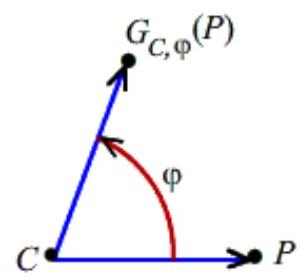
\includegraphics[max width=3cm]{2023_04_25_301d1803eaf1bc74cfd9g-080(1)}
\end{center}
\observacion
\begin{itemize}
\item $G_{C, \varphi}$ son movimientos, ya que son la única afinidad con $G_{C, \varphi}(C) = C$ y $\vec{G_{C, \varphi}} = G_\varphi \in \mathcal{O}^+(V)$.
\item $G_{V,0} = \operatorname{Id}_A, \; \forall V \in \mathbb{A}$.
\end{itemize}

\subsubsection{Proposición}
\noindent Si $\varphi \neq 0$, es $C$, el único punto fijo del giro de centro $C$ y ángulo $\varphi$.

\demostracion

Se tiene
$$
G_{C, \varphi}(P)=P \Longleftrightarrow C+G_{\varphi}(\overrightarrow{C P})=P \Longleftrightarrow G_{\varphi}(\overrightarrow{C P})=\overrightarrow{C P} \xLeftrightarrow{\varphi \neq 0} \overrightarrow{C P}=0 \Longleftrightarrow C=P
$$

\subsubsection{Definición}
Se llama simetría respecto a la recta $r=A+\langle u\rangle$ a la aplicación $S_{r}: \mathbb{A} \rightarrow \mathbb{A}$, dada por $S_{r}(P)=A+S_{\langle u\rangle}(\overrightarrow{A P})$, donde $S_{\langle u\rangle}$ es la simetría respecto a $\langle u\rangle$.
\begin{center}
	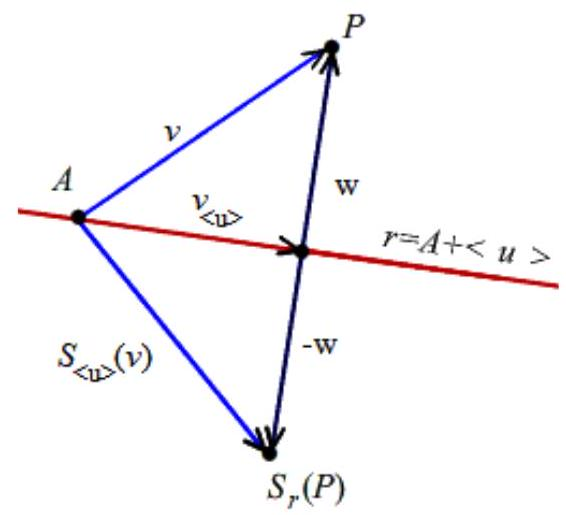
\includegraphics[max width=5cm]{2023_04_25_301d1803eaf1bc74cfd9g-080}
\end{center}
\observacion

$S_r$ es el único movimiento con $S_r(A) = A$, $\vec{S_r}$ = $S_{\langle u \rangle} in \mathcal{O}^-(V)$. Veamos que $S_r$ no depende de $A$: $A^{\prime} \in r$, entonces $A+S_{\langle u\rangle}(\overrightarrow{A P})=A^{\prime}+S_{\langle u\rangle}\left(\overrightarrow{A^{\prime} P}\right)$. En efecto, dado que $\overrightarrow{A A^{\prime}} \in\langle u\rangle$, se tiene $S_{\langle u\rangle}\left(\overrightarrow{A A^{\prime}}\right)=\overrightarrow{A A^{\prime}}$ y por tanto $S_{\langle u\rangle}(\overrightarrow{A P})=S_{\langle u\rangle}\left(\overrightarrow{A A^{\prime}+A^{\prime} P}\right)=\overrightarrow{A A^{\prime}}+S_{\langle u\rangle}\left(\overrightarrow{A^{\prime} P}\right)$. En particular, $S_r(A') = A', \; \forall A' \in r$.

\subsubsection{Proposición}
Los únicos puntos fijos de la simetría $S_{r}$ son los puntos de $r$.

\demostracion

Se tiene
$$
S_{r}(P)=P \Longleftrightarrow A+S_{\langle u\rangle}(\overrightarrow{A P})=P \Longleftrightarrow S_{\langle u\rangle}(\overrightarrow{A P})=\overrightarrow{A P} \Longleftrightarrow \overrightarrow{A P} \in\langle u\rangle \Longleftrightarrow P \in r
$$

3.4.6. Definición. Se llama simetría deslizante respecto a la recta $r=A+\langle u\rangle$ y vector de traslación $v \in\langle u\rangle, v \neq 0$ a la aplicación $S_{r, v}=t_{v} \circ S_{r}$, donde $S_{r}$ es la simetría respecto a la recta $r$.

\begin{center}
	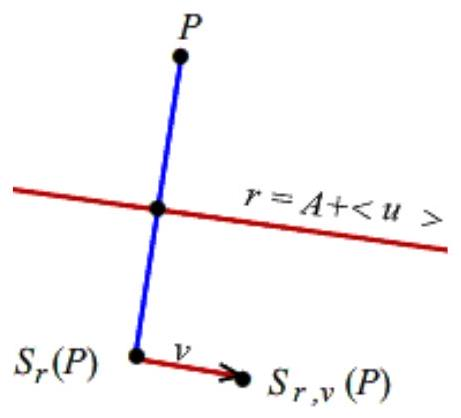
\includegraphics[max width=\textwidth]{2023_04_25_301d1803eaf1bc74cfd9g-081}
\end{center}

Por $3.3 .3(3), S_{r}$ es un movimiento.

3.4.7. Proposición. La simetría deslizante $S_{r, v}$ no tiene puntos fijos.

Demostración. Razonemos por reducción al absurdo: Si $P$ es un punto fijo de $S_{r, v}$, entonces

$$
S_{r, v}(P)=P \Longleftrightarrow A+S_{\langle u\rangle}(\overrightarrow{A P})+v=P \Longleftrightarrow S_{\langle u\rangle}(\overrightarrow{A P})+v=\overrightarrow{A P}
$$

Dado que además, $S_{\langle u\rangle}(\overrightarrow{A P})=\overrightarrow{A P}+v$, se tiene $v=0$, lo cual contradice la definición de simetría deslizante.

3.4.8. Ejercicio. Prueba que la descomposición de una simetría deslizante como composición de la simetría respecto a una recta y una traslación por un vector de la dirección de la recta es única.

3.4.9. Teorema. (Teorema de clasificación de los movimientos del plano afín euclídeo) Sea A un plano afín euclídeo orientado sobre $V, M: \mathbb{A} \rightarrow \mathbb{A}$ un movimiento y $A$ un punto cualquiera de $\mathbb{A}$. Pongamos $V_{1}=\ker\left(\vec{M}-\mathrm{id}_{V}\right)$. Se tiene

(1) Si $\vec{M}=\operatorname{id}_{V}$, entonces $M=t_{v}$ es una traslación con $v=\overrightarrow{A M(A)}$.

(2) Si $\vec{M} \in \mathbb{O}^{+}(V)$ y $\vec{M} \neq \mathrm{id}_{V}$, entonces $\vec{M}$ es un giro de ángulo $\varphi \neq 0$ y $M$ es el giro de centro $C=A-v$ y ángulo $\varphi$, siendo $v$ el vector que verifica $\vec{M}(v)-v=\overrightarrow{A M(A)}$.

(3) Si $\vec{M} \in \mathbb{O}^{-}(V)$ y $\overrightarrow{A M(A)} \in\left(V_{1}\right)^{\perp}$, entonces $M$ es la simetría respecto a la recta $r=A+$ $\frac{1}{2} \overrightarrow{A M(A)}+V_{1}$



















\end{document}